% Abbring & Van den Berg (2003): reading-group presentation.
% Build slides:             pdflatex slides.tex
% Build slides + notes:     pdflatex -jobname=slides_with_notes "\def\withnotes{1}% Abbring & Van den Berg (2003): reading-group presentation.
% Build slides:             pdflatex slides.tex
% Build slides + notes:     pdflatex -jobname=slides_with_notes "\def\withnotes{1}% Abbring & Van den Berg (2003): reading-group presentation.
% Build slides:             pdflatex slides.tex
% Build slides + notes:     pdflatex -jobname=slides_with_notes "\def\withnotes{1}% Abbring & Van den Berg (2003): reading-group presentation.
% Build slides:             pdflatex slides.tex
% Build slides + notes:     pdflatex -jobname=slides_with_notes "\def\withnotes{1}\input{slides.tex}"
% (or just run ./build.sh)
\documentclass[aspectratio=169,10pt]{beamer}
\ifdefined\withnotes
  \setbeameroption{show notes}
\fi
\setbeamertemplate{navigation symbols}{}
\setbeamertemplate{footline}[frame number]
\setbeamertemplate{note page}{\vspace{1em}\small\insertnote}

\usepackage{amsmath,amssymb,booktabs,tikz}
\usetikzlibrary{arrows.meta,positioning}
\graphicspath{{../figures/}}

\newcommand{\E}{\mathbb{E}}
\newcommand{\1}{\mathbf{1}}
\newcommand{\R}{\mathbb{R}}
\newcommand{\Lap}{\mathcal{L}}
\newcommand{\cov}{\operatorname{Cov}}

\title{The Nonparametric Identification of Treatment Effects in Duration Models}
\subtitle{Abbring \& Van den Berg (2003, \textit{Econometrica})}
\author{Econometrics Reading Group}
\date{}

\begin{document}

% =====================================================================
\begin{frame}
  \titlepage
\note{
\textbf{How to read these notes.} Every slide has a note like this one. The notes say where the slide's content comes from, what the previous slide left unresolved, and what this slide adds. Read slides + notes in order: the argument is cumulative.

\medskip
\textbf{The plan in one sentence.} We want the effect of a treatment that arrives at a random time during a spell. The difficulty is selection on unobservables. The paper's answer is that the \emph{pre-treatment} part of the data is a competing-risks problem; with hazard structure, that part reveals the distribution of unobserved types among those at risk; knowing that distribution lets us strip the selection out of the \emph{post-treatment} part.

\medskip
\textbf{Notation changes relative to the paper.} We write the data as four interpretable objects ($P_0, h_Y, h_S, P_1$) instead of the paper's sub-survival functions $(Q_S,Q_Y)$; the mapping is in the appendix. We write $D(y\mid s,x)$ for the integrated post-treatment hazard (the paper uses $\Upsilon$). We write the bivariate Laplace transform as $\Lap(a,b)$ and its partial derivatives as $\Lap_a,\Lap_b,\Lap_{ab}$.
}
\end{frame}

% =====================================================================
\begin{frame}{The question}
  \textbf{Running example.} An unemployed worker may receive a benefit sanction at a random time $S$ during the spell. Outcome: unemployment duration $Y$.

  \medskip
  \textbf{Target.} The causal effect of the sanction on the \emph{exit rate} to work.

  \medskip
  \textbf{Why this is hard}
  \begin{enumerate}
    \item \textbf{Dynamic treatment:} no fixed treated group; everyone is untreated until $S$.
    \item \textbf{Treatment is censored:} if you find a job before your sanction date, $S$ is never seen.
    \item \textbf{Selection on unobservables:} low-motivation workers get sanctioned earlier \emph{and} exit more slowly.
    \item \textbf{No credible instrument:} whatever shifts sanctions, the worker likely sees and reacts to.
  \end{enumerate}

  \medskip
  \textbf{Punchline.} The \emph{timing} of $S$ relative to $Y$ does the job of the instrument, at the price of structure on hazards.
\note{
Point 4 is the paper's own argument (Section 1) against IV. If a variable affects treatment and the agent can see it, a forward-looking agent adjusts behaviour, so the variable also affects the outcome hazard directly. Exclusion restrictions are therefore hard to defend in dynamic settings.

Point 2 explains why the data are unusual. We see $S$ only for people with $S<Y$. This censoring is not a nuisance to be fixed; it is what turns the pre-treatment data into a competing-risks problem (slide 10).

The punchline is what the rest of the talk earns. Keep the four difficulties visible: each later assumption addresses one of them.
}
\end{frame}

% =====================================================================
\begin{frame}{Primer 1: hazards and dynamic selection}
  \begin{columns}[T]
    \begin{column}{0.47\textwidth}
      \textbf{Hazard} of a duration $T$:
      \[ \theta(t)=\lim_{dt\downarrow0}\tfrac{\Pr(T\in[t,t+dt)\mid T\ge t)}{dt} \]
      $\Lambda(t)=\int_0^t\theta$, \quad $\Pr(T>t)=e^{-\Lambda(t)}$.

      \smallskip
      In every instant, each survivor flips a coin with success probability $\theta(t)\,dt$.

      \medskip
      \textbf{Heterogeneity:} $\theta(t\mid V)=\lambda(t)\,V$. Then the hazard we \emph{observe} is
      \[ \bar\theta(t)=\lambda(t)\;\E[V\mid T\ge t], \]
      and $\E[V\mid T\ge t]$ \textbf{falls}: high-$V$ people leave first.
    \end{column}
    \begin{column}{0.53\textwidth}
      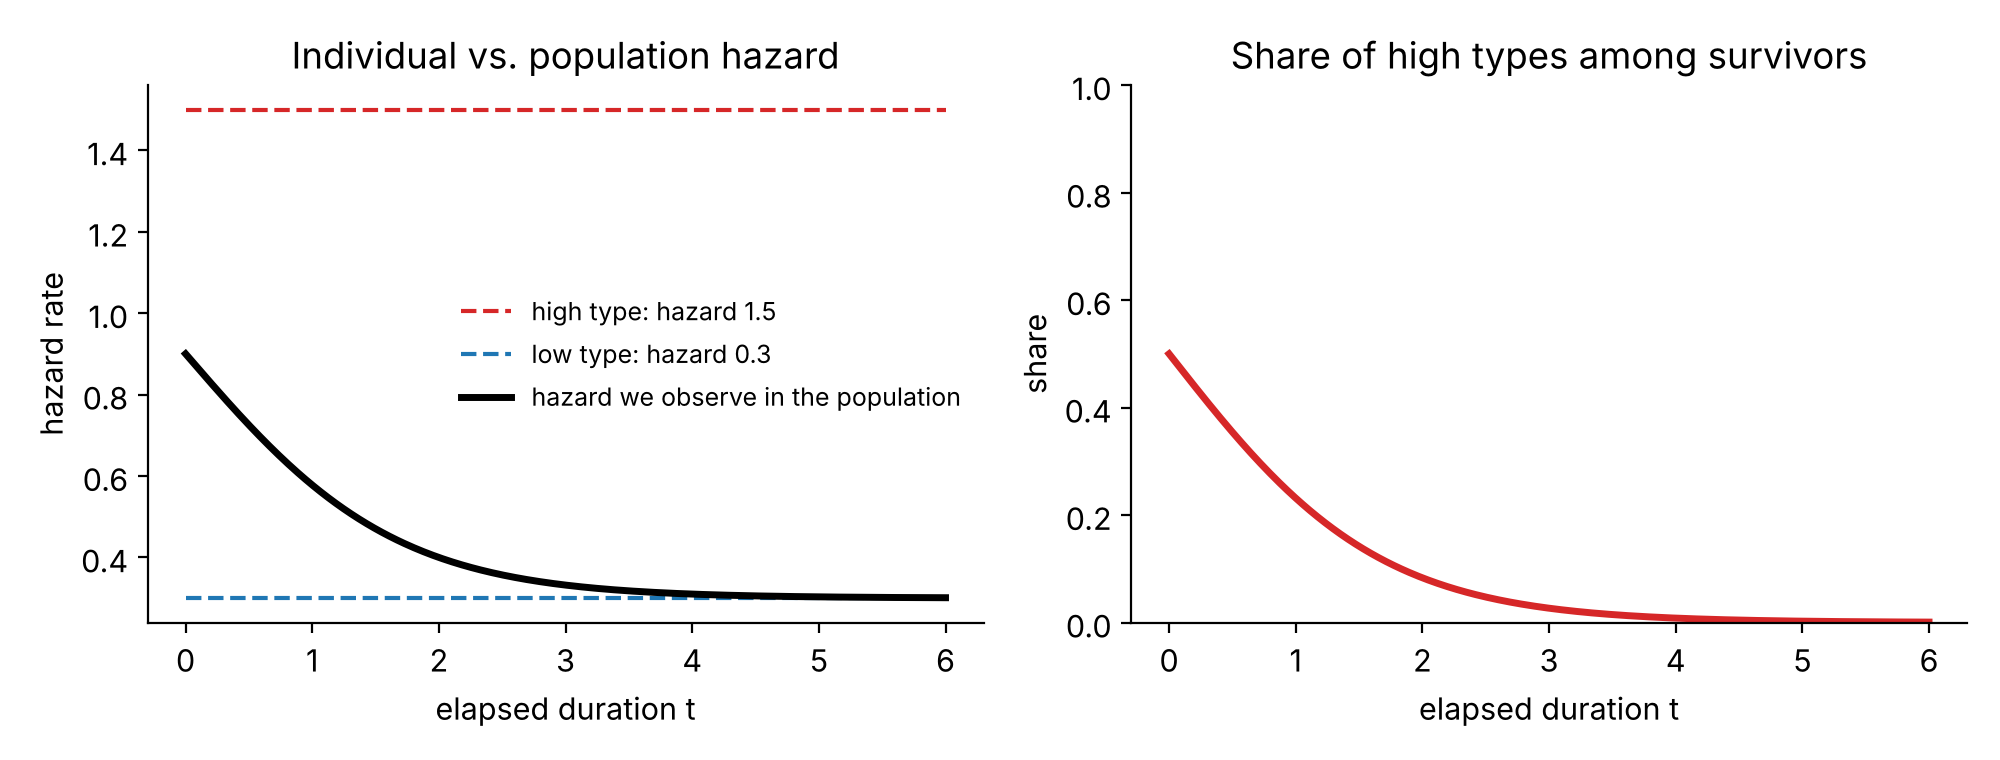
\includegraphics[width=\linewidth]{fig1_dynamic_selection.png}
    \end{column}
  \end{columns}

  \medskip
  \textbf{Trap or sorting?} A falling exit rate can be true duration dependence ($\lambda\downarrow$) or composition ($\E[V\mid T\ge t]\downarrow$). This is Heckman's \emph{true vs.\ spurious state dependence}, in continuous time.
\note{
\textbf{Derivation of the observed hazard.} The survival function is $\Pr(T>t)=\E[e^{-V\Lambda(t)}]$, with $\Lambda(t)=\int_0^t \lambda$. The population hazard is $-\frac{d}{dt}\log\Pr(T>t)=\lambda(t)\,\E[Ve^{-V\Lambda(t)}]/\E[e^{-V\Lambda(t)}]$. The ratio is the mean of $V$ under weights $e^{-V\Lambda(t)}$, i.e.\ $\E[V\mid T\ge t]$. The weight $e^{-V\Lambda(t)}$ is the probability that a type-$V$ person is still there. That is the whole idea of dynamic selection.

\textbf{Why it matters for treatment effects.} The people still unemployed and untreated at month 6 are a selected group. Comparing ``treated at month 6'' with ``not yet treated at month 6'' is only valid if we know how both groups were selected up to month 6. Every identification step below is about learning that selection.

\textbf{Figure.} Two types with \emph{constant} hazards 0.3 and 1.5 produce a population hazard that falls from 0.9 to 0.3. Nobody's hazard changes; only the composition does.

\textbf{The coin-flip view} matters later. Conditional on the hazard, the moment of the event is pure chance. This is the source of the ``randomization'' the paper exploits (footnote 15).
}
\end{frame}

% =====================================================================
\begin{frame}{Primer 2: the MPH model and the Laplace-transform toolkit}
  \textbf{Mixed proportional hazard:} $\theta(t\mid x,V)=\lambda(t)\,\varphi(x)\,V$, \quad $V\sim G$, \ $V\perp x$. Then
  \[ \Pr(T>t\mid x)=\E\big[e^{-V\varphi(x)\Lambda(t)}\big]=\Lap\big(\varphi(x)\Lambda(t)\big),\qquad \Lap(a):=\E[e^{-aV}]. \]
  \textbf{Toolkit.} $e^{-aV}$ is the probability that type $V$ survives to index $a$. So derivatives of $\log\Lap$ are \emph{moments among survivors}. In two dimensions, $\Lap(a,b)=\E[e^{-aV_Y-bV_S}]$:
  \[
    -\partial_a\log\Lap=\E[V_Y\mid\text{surv.}],\qquad
    -\partial_b\log\Lap=\E[V_S\mid\text{surv.}],\qquad
    \partial^2_{ab}\log\Lap=\cov(V_Y,V_S\mid\text{surv.}).
  \]
  \textbf{Single-risk identification (Elbers \& Ridder 1982), in 3 steps}
  \begin{enumerate}
    \item $t\downarrow0$: nobody has been selected out yet, so hazard ratios across $x$ give $\varphi(x)$ (needs $\E V<\infty$).
    \item At $t^*$ with $\Lambda(t^*)=1$: $\Pr(T>t^*\mid x)=\Lap(\varphi(x))$. Varying $x$ traces $\Lap$, hence $G$.
    \item Any $t$: solve $\Pr(T>t\mid x)=\Lap(\varphi(x)\Lambda(t))$ for $\Lambda(t)$.
  \end{enumerate}
  \textbf{We will run exactly this logic in two dimensions.}
\note{
\textbf{Where the toolkit comes from.} $\log\Lap(a,b)$ is the cumulant generating function of $(-V_Y,-V_S)$, evaluated under tilting by $e^{-aV_Y-bV_S}$. First derivative: $\partial_a\log\Lap=-\E[V_Ye^{-aV_Y-bV_S}]/\Lap=-\E_w[V_Y]$. Differentiate again in $b$: $\partial_b(-\E_w[V_Y])=\E_w[V_YV_S]-\E_w[V_Y]\E_w[V_S]=\cov_w(V_Y,V_S)$. The weights $w$ are survival probabilities, so ``$\E_w$'' means ``among survivors''. Two consequences we use repeatedly:
(i) the observed hazard is $\lambda\varphi\times(-\partial_a\log\Lap)$;
(ii) the dependence between $V_Y$ and $V_S$ among survivors (the selection) is a cross-derivative.

\textbf{Step 1 in detail.} The hazard is $\lambda(t)\varphi(x)\E[V\mid T\ge t,x]$. As $t\downarrow0$, $\E[V\mid T\ge t,x]\to\E[V]$, which is finite by assumption and the same for all $x$ because $V\perp x$. The ratio across $x$ and $x^*$ therefore tends to $\varphi(x)/\varphi(x^*)=\varphi(x)$. Note that identification uses the behaviour of short durations, where data are thin (critique on slide 17).

\textbf{Step 2.} The normalization $\Lambda(t^*)=1$ fixes the scale. Once $\varphi$ is known, $x\mapsto\Pr(T>t^*\mid x)$ is $\Lap$ evaluated at known points. Varying $x$ traces $\Lap$ on an interval. Laplace transforms are analytic, so $\Lap$ is then pinned down everywhere, and it determines $G$ uniquely.

\textbf{Step 3.} $\Lap$ is strictly decreasing, so invert.
}
\end{frame}

% =====================================================================
\begin{frame}{Set-up: potential outcomes indexed by treatment time}
  \begin{itemize}
    \item Treatments are dates $s\in[0,\infty]$ ($s=\infty$: never). Potential outcomes $Y^*(s)$; observed $Y=Y^*(S)$.
    \item \textbf{No anticipation:} $\theta_{Y^*(s)}(t)=\theta_{Y^*(s')}(t)$ for $t\le\min(s,s')$. A future treatment date does not affect today's hazard.\\
      Reacting to the sanction \emph{regime} is allowed (it is in every $Y^*(s)$), so the effect is \emph{``treated at $s$ vs.\ later, under this regime''}.
  \end{itemize}
  \begin{center}
  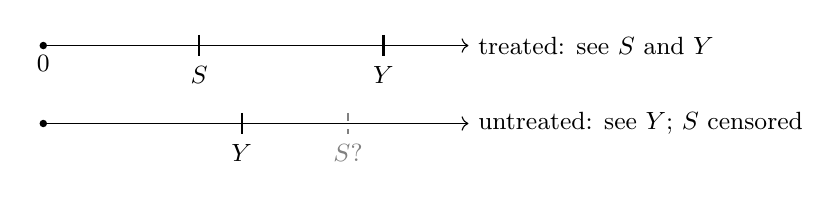
\begin{tikzpicture}[scale=0.9]
    \draw[->] (0,0) -- (6,0) node[right] {\small treated: see $S$ and $Y$};
    \fill (0,0) circle (1.5pt) node[below] {\small 0};
    \draw[thick] (2.2,0.15) -- (2.2,-0.15) node[below] {\small $S$};
    \draw[thick] (4.8,0.15) -- (4.8,-0.15) node[below] {\small $Y$};
    \draw[->] (0,-1.1) -- (6,-1.1) node[right] {\small untreated: see $Y$; $S$ censored};
    \fill (0,-1.1) circle (1.5pt);
    \draw[thick] (2.8,-0.95) -- (2.8,-1.25) node[below] {\small $Y$};
    \draw[dashed,gray] (4.3,-0.95) -- (4.3,-1.25) node[below] {\small $S$?};
  \end{tikzpicture}
  \end{center}
  \textbf{What the data reveal} (all conditional on $x$):
  \begin{itemize}
    \item $P_0(t)=\Pr(Y>t,S>t)$: nothing has happened by $t$;
    \item $h_Y(t)$, $h_S(t)$: rate of exiting untreated / of being treated, among those with nothing yet;
    \item $P_1(y\mid s)=\Pr(Y>y\mid S=s,\,Y>s)$: post-treatment survival of the \textbf{cohort treated at $s$}.
  \end{itemize}
  \textbf{Fact (Prop.~1):} any such data can be rationalized with no anticipation \emph{and} random assignment. So no anticipation is untestable, and we need a model of selection.
\note{
\textbf{Why index potential outcomes by a date.} A dynamically assigned binary treatment is really a continuum of mutually exclusive treatments, ``treated at $s$''. This is exactly the staggered-adoption set-up, where potential outcomes are indexed by the adoption cohort $g$ (slide 18).

\textbf{No anticipation.} The paper states it for integrated hazards; hazard paths agreeing up to $\min(s,s')$ is the same thing. In biostatistics this is a mild consistency condition. In economics it is behavioural: if a worker knows the sanction date and searches harder beforehand, it fails. If information arrives before treatment, the paper suggests treating the \emph{information shock} as the treatment.

\textbf{The data objects.} These four objects are equivalent to the paper's $(Q_S,Q_Y)$; see the appendix. The pre-treatment objects ($P_0,h_Y,h_S$) are classic \emph{competing-risks} data: two things can happen and we see which happens first. $P_1$ is the only place where the treatment effect can appear.

\textbf{Proposition 1 (de-emphasized).} By the Tsiatis/Miller result, any competing-risks data are generated by some \emph{independent} pair of latent durations. Use that pair for the pre-treatment part, and define the post-treatment hazard to match $P_1$. The result is a model with random assignment and no anticipation that fits the data perfectly. Two lessons: selection cannot be told from causality without structure, and anticipation cannot be detected. The paper's job-search illustration is in the appendix.
}
\end{frame}

% =====================================================================
\begin{frame}{The model}
  \textbf{Assumption 2 (selection on $(x,V)$):} $Y^*(\cdot)\perp S \mid (x,V)$, with $V$ time-invariant.

  \medskip
  \textbf{Model 1a.}
  \[
  \theta_Y(t\mid s,x,V)=\lambda_Y(t)\,\varphi_Y(x)\,V_Y\cdot\delta(t\mid s,x)^{\1\{t>s\}},\qquad
  \theta_S(t\mid x,V)=\lambda_S(t)\,\varphi_S(x)\,V_S,
  \]
  with $(V_Y,V_S)\sim G$ \textbf{arbitrarily dependent}, independent of $x$.

  \medskip
  \begin{itemize}
    \item Two MPH hazards. Their link through $\cov(V_Y,V_S)$ is the \textbf{selection on unobservables}.
    \item $\delta$ is the \textbf{causal effect}: a hazard multiplier after treatment. It may vary with $t$, $s$ (hence with $t-s$) and $x$, but not with $V$.
    \item No anticipation is built in: $\delta$ only acts for $t>s$.
    \item The same $x$ enters both hazards, so there is \textbf{no exclusion restriction}. $\lambda$'s, $\varphi$'s, $G$, $\delta$ are all nonparametric.
  \end{itemize}

  \medskip
  \textbf{Assn.~3:} $\{(\varphi_Y(x),\varphi_S(x))\}$ contains an open set of $\R^2$. \quad \textbf{Assn.~4:} $\E V_Y,\E V_S<\infty$.\\
  Normalizations: $\varphi(x^*)=1$, $\Lambda(t^*)=1$.
\note{
\textbf{How the model emerges from the set-up.} No anticipation says pre-treatment hazards do not depend on $s$. Assumption 2 says all dependence between $Y$ and $S$ runs through $(x,V)$. Together they imply: conditional on $(x,V)$, $Y$ and $S$ are linked \emph{only} through the causal factor $\delta$. That is why $\delta$ can be called a treatment effect.

\textbf{Why hazard-based assignment matters.} $S$ is modelled by a hazard, not by a threshold-crossing rule. So even conditional on $(x,V)$, $S$ is random: $\varphi_S(x)V_S\Lambda_S(S)$ is a unit exponential independent of $(x,V)$. This random component moves $S$ around without affecting $Y$ except through treatment. It is the analogue of an instrument (slide 8).

\textbf{Assumption 3 is not an exclusion restriction, but it is not free.} The covariates must move the two hazards \emph{non-proportionally}. With $\varphi_j(x)=e^{x'\beta_j}$ you need at least two continuous covariates and $(\beta_Y\ \beta_S)$ of full rank.

\textbf{Allowed but not shown:} mass points of $V$ at zero (never treated / never exit). Also $\Pr(Y=S)=0$ (continuous time, no ties).
}
\end{frame}

% =====================================================================
\begin{frame}{The selection problem at the moment of treatment}
  Fix a duration $s$. Write $a_s=\varphi_Y(x)\Lambda_Y(s)$, $b_s=\varphi_S(x)\Lambda_S(s)$.

  \medskip
  \textbf{Who is still at risk} (nothing happened by $s$):\quad $dG_{R_s}(v)\propto e^{-a_s v_Y-b_s v_S}\,dG(v)$.\\[2pt]
  \textbf{Who is treated at $s$:} the risk set, reweighted by the treatment intensity, \quad $dG_{s}(v)\propto v_S\,dG_{R_s}(v)$.

  \medskip
  \textbf{Exit hazards right at $s$:}
  \[
  \underbrace{\lambda_Y(s)\varphi_Y(x)\,\E_{R_s}[V_Y]}_{\text{not yet treated}}
  \qquad\text{vs.}\qquad
  \underbrace{\lambda_Y(s)\varphi_Y(x)\,\delta(s\mid s,x)\,\E_{s}[V_Y]}_{\text{just treated}}
  \]
  \[
  \frac{\text{just treated}}{\text{not yet treated}}
  \;=\;\delta(s\mid s,x)\times\underbrace{\Big(1+\frac{\cov_{R_s}(V_Y,V_S)}{\E_{R_s}[V_Y]\,\E_{R_s}[V_S]}\Big)}_{\text{selection factor}}
  \]
  \begin{itemize}
    \item If $V_Y\perp V_S$ among survivors, timing is as good as random at $s$: the ratio \emph{is} the causal effect.
    \item Otherwise we need the \textbf{joint distribution of types among survivors}. The pre-treatment data will supply it.
  \end{itemize}
\note{
\textbf{This slide is the heart of the paper's logic.} It reduces the selection problem to one object.

\textbf{Derivation.} Being at risk at $s$ means $Y>s$ and $S>s$. Given $V$, no anticipation means $Y$'s hazard before $s$ is the untreated one, so the probability of being at risk is $e^{-a_sV_Y}e^{-b_sV_S}$ (Assumption 2 lets the two terms multiply). By Bayes' rule, the type distribution in the risk set is $G$ reweighted by that probability. Among those at risk, the chance of being treated in $[s,s+ds)$ is $\lambda_S(s)\varphi_S(x)V_S\,ds$. So the treated cohort is the risk set reweighted by $V_S$.

The mean of $V_Y$ in the treated cohort is
$\E_s[V_Y]=\E_{R_s}[V_YV_S]/\E_{R_s}[V_S]=\E_{R_s}[V_Y]+\cov_{R_s}(V_Y,V_S)/\E_{R_s}[V_S]$.
Divide by $\E_{R_s}[V_Y]$ to get the selection factor.

\textbf{Reading it.} Suppose low-motivation people (low $V_Y$) are sanctioned more (high $V_S$), so the covariance is negative. Then the just-treated have low $V_Y$, and the naive comparison \emph{understates} a positive effect of sanctions on exit. This is the classic ``Heckman selection'' structure, with a control-function-like correction factor.

\textbf{The ratio on the left is data.} The hazard of the just-treated is $-\partial_y\log P_1(y\mid s)$ as $y\downarrow s$; the hazard of the not-yet-treated is $h_Y(s)$. So everything hinges on the selection factor, a feature of the joint distribution of $(V_Y,V_S)$ among those at risk at $s$.
}
\end{frame}

% =====================================================================
\begin{frame}{Timing as an instrument}
  \footnotesize
  \begin{tabular}{p{0.2\textwidth}p{0.29\textwidth}p{0.41\textwidth}}
    \toprule
    & Static selection / IV & Timing of events \\
    \midrule
    Exogenous variation in treatment
    & excluded variable $Z$
    & the timing shock: given $(x,V)$, $S=\Lambda_S^{-1}\!\big(\tfrac{E_S}{\varphi_S(x)V_S}\big)$, $E_S\sim\text{Exp}(1)$ \\[3pt]
    What is excluded from the outcome
    & the \emph{variable} $Z$
    & the \emph{shock} $E_S$ (via Assn.~2) \\[3pt]
    Correcting for who selects in
    & control function $\E[U\mid D=1,Z]$
    & selection factor / $G_s$, from the competing-risks data \\[3pt]
    Covariate requirement
    & $Z$ shifts $D$, not $Y$
    & $x$ shifts both hazards, \emph{non-proportionally} (Assn.~3) \\
    \bottomrule
  \end{tabular}

  \normalsize
  \bigskip
  \textbf{Why timing is informative.} The treatment acts only \emph{after} $S$; $V$ acts \emph{throughout}.
  \begin{itemize}
    \item Causal effect $\Rightarrow$ \textbf{local} dependence: exits bunch right after $S$, \emph{whenever} $S$ occurs.
    \item Selection $\Rightarrow$ \textbf{global} dependence: early-treated people are early leavers in general.
  \end{itemize}
  In a static latent-index model the treatment effect needs an exclusion restriction. Here the timing replaces it.
\note{
\textbf{The point of the table.} An IV design needs two things: (i) variation in treatment that is unrelated to the outcome's unobservables, and (ii) a way to handle the fact that the people who take treatment are selected.

(i) In a static threshold model $D=\1\{\mu(Z)>U\}$, treatment is deterministic given $(Z,U)$, so exogenous variation must come from an excluded $Z$. With hazard-based assignment, treatment \emph{timing} is still random given $(x,V)$. The representation uses the fact that $\varphi_S(x)V_S\Lambda_S(S)$ is unit exponential. The exclusion restriction has not disappeared: it moved from an observed variable to an unobserved shock. Assumption 2 says the timing shock $E_S$ is independent of everything that drives $Y$. Be candid about this in the talk.

(ii) The selection correction is the analogue of a control function. Here it is not estimated from an excluded instrument; it comes from the competing-risks part of the data (next three slides).

\textbf{Local vs.\ global.} This is the paper's own intuition (Section 3.2) and the basis of the companion paper on testing the sign of $\delta$. The figure on the next slide makes it concrete.
}
\end{frame}

% =====================================================================
\begin{frame}{What the data look like}
  \centering
  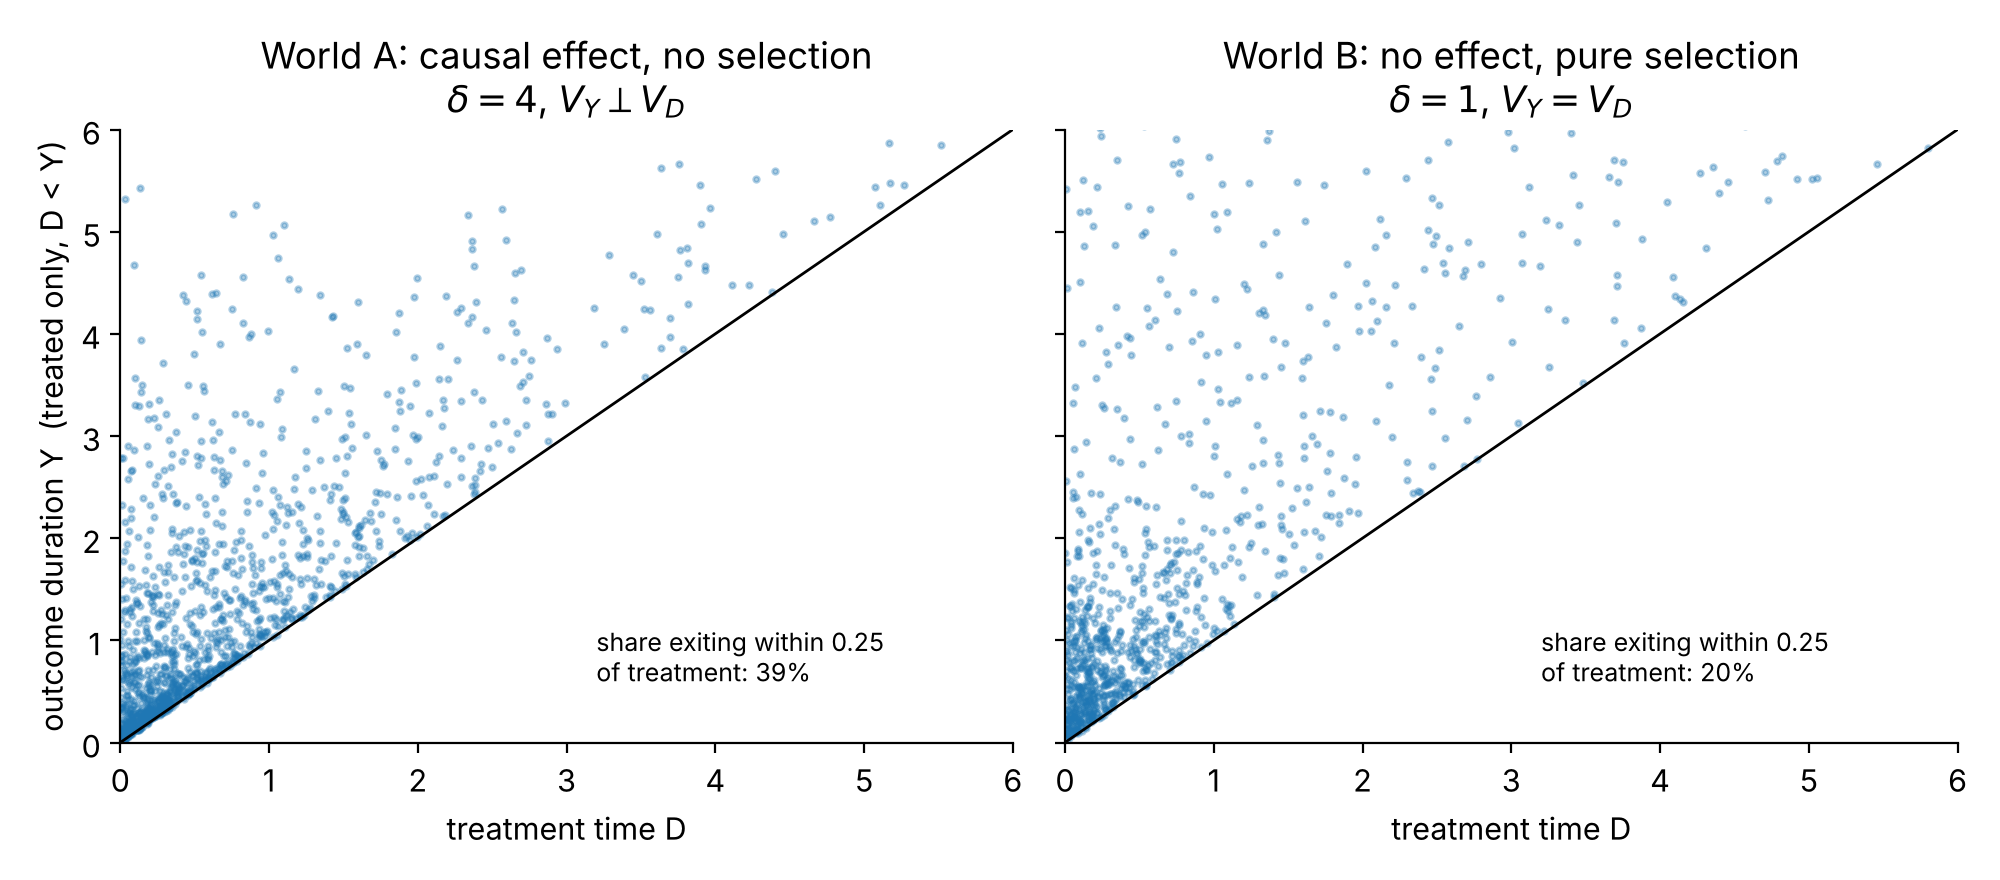
\includegraphics[width=0.85\linewidth]{fig3_local_vs_global.png}

  \raggedright\small
  Treated observations only. Left: $\delta=4$, independent frailties. Right: $\delta=1$, $V_Y=V_S$. A causal effect makes points hug the diagonal \emph{at every $S$}. Selection produces quick exits only where high types are concentrated (small $S$).
\note{
\textbf{Simulation.} Two types (0.25 and 2), constant baseline hazards. World A: types for $Y$ and $S$ drawn independently, and treatment multiplies the exit hazard by 4. World B: one common type, no effect.

Both worlds show a positive association between $S$ and $Y$, and in both some people exit quickly after treatment. The difference is \emph{where} the quick exits are. In A they occur after treatment at any $S$; in B they are concentrated at small $S$, where the high types still are. The formal argument quantifies exactly this: how many quick post-treatment exits would we expect from selection alone, given the types at risk at $s$?

Script: \texttt{figures/make\_figures.py}.
}
\end{frame}

% =====================================================================
\begin{frame}{The pre-treatment data are a competing-risks problem}
  Before treatment there are two latent clocks: $Y^0$ (exit if never treated) and $S$. Their joint survival is
  \[ \Pr(Y^0>y,\,S>s\mid x)=\Lap\big(\varphi_Y(x)\Lambda_Y(y),\;\varphi_S(x)\Lambda_S(s)\big). \qquad \text{($\delta$ does not appear!)}\]
  We only see the \emph{first} event: the diagonal $y=s=t$, i.e.\ $P_0(t\mid x)=\Lap(a_t(x),b_t(x))$, plus which event it was.

  \smallskip
  \textbf{Tsiatis (1975):} without structure, any such data are generated by \emph{independent} clocks. The dependence, i.e.\ the selection, is unidentified.

  \begin{center}
    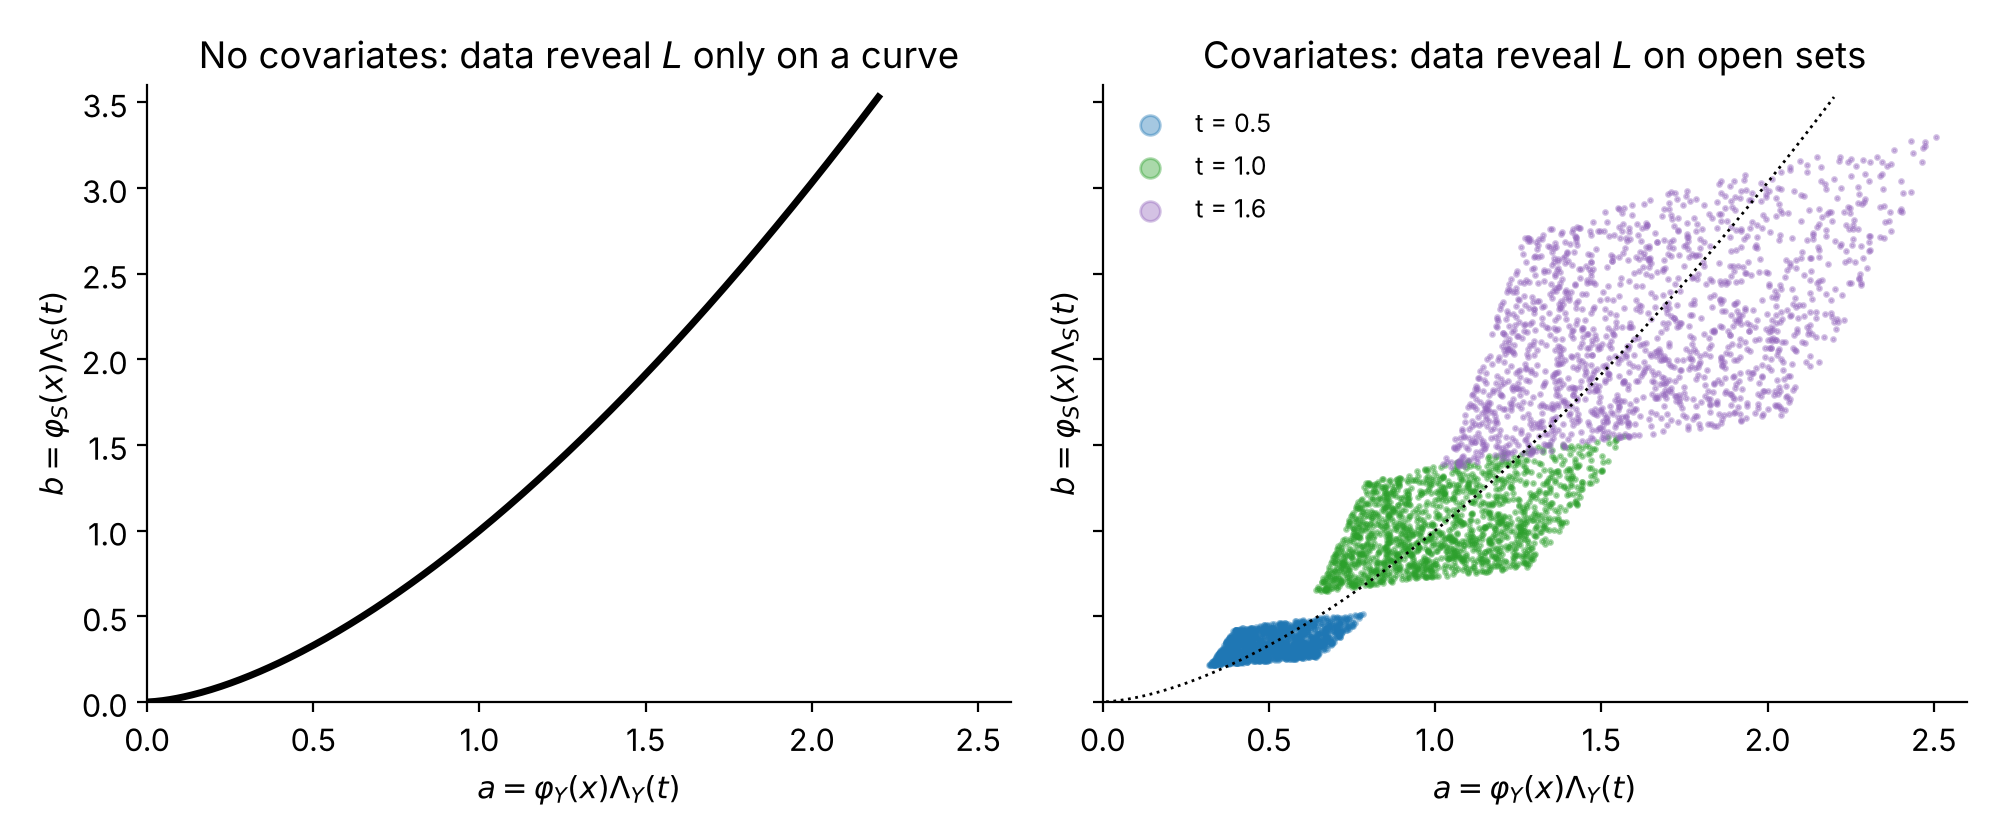
\includegraphics[width=0.56\linewidth]{fig4_competing_risks_geometry.png}
  \end{center}
  \vspace{-6pt}
  \small Without $x$, the data reveal $\Lap$ only along a curve $t\mapsto(\Lambda_Y(t),\Lambda_S(t))$. A curve cannot pin down a function of two variables. With $x$ shifting the two hazards separately, the data reveal $\Lap$ on \emph{open sets}.
\note{
\textbf{Why this is the crucial step.} Slide 7 showed that everything hinges on the joint distribution of $(V_Y,V_S)$. The only place to learn it without using the outcome we want to explain is the pre-treatment period. There, by no anticipation, nothing causal is going on. We just watch two clocks race.

\textbf{The joint survival.} Given $V$, the two clocks are independent with integrated hazards $\varphi_Y\Lambda_YV_Y$ and $\varphi_S\Lambda_SV_S$. Integrating over $G$ gives the bivariate Laplace transform evaluated at the two indices.

\textbf{Geometry of non-identification.} With no covariates, data at duration $t$ tell us $\Lap$ at one point $(\Lambda_Y(t),\Lambda_S(t))$. As $t$ varies we learn $\Lap$ along a curve, plus the slopes of $\Lap$ in the two directions along that curve (from the cause-specific hazards). Many bivariate distributions agree on those values, including independent ones. That is Tsiatis' result.

\textbf{How covariates break it.} At a fixed $t$, varying $x$ moves the point to $(\varphi_Y(x)\Lambda_Y(t),\varphi_S(x)\Lambda_S(t))$. If the two $\varphi$'s move independently (Assumption 3), the point sweeps out a two-dimensional patch. Knowing an analytic function on any open patch determines it everywhere. This is why Assumption 3 must be two-dimensional, and it is what makes the selection identified.
}
\end{frame}

% =====================================================================
\begin{frame}{Identifying the competing-risks part (Prop.~2): three steps}
  \textbf{Step 1: $\varphi$'s from short durations} (nobody has been selected out yet):
  \[ \frac{h_Y(t\mid x)}{h_Y(t\mid x^*)}=\frac{\varphi_Y(x)\,\E[V_Y\mid R_t,x]}{\E[V_Y\mid R_t,x^*]}\;\xrightarrow{\;t\downarrow0\;}\;\varphi_Y(x),\qquad\text{same for }\varphi_S. \]
  Uses \emph{which} event happened and $\E V<\infty$.

  \medskip
  \textbf{Step 2: $G$ at the normalization date} ($\Lambda_Y(t^*)=\Lambda_S(t^*)=1$):
  \[ P_0(t^*\mid x)=\Lap\big(\varphi_Y(x),\varphi_S(x)\big). \]
  Known points fill an open set (Assn.~3), so $\Lap$ is known there. $\Lap$ is real-analytic, so it is known on $(0,\infty)^2$, and $\Lap$ determines $G$, \textbf{including the dependence between $V_Y$ and $V_S$}.

  \medskip
  \textbf{Step 3: baselines.} For every $t$, $(\Lambda_Y(t),\Lambda_S(t))$ is the unique $(a,b)$ with
  \[ P_0(t\mid x)=\Lap\big(\varphi_Y(x)\,a,\;\varphi_S(x)\,b\big)\quad\text{for all }x. \]

  \medskip
  $\Rightarrow$ $\lambda_Y,\lambda_S,\varphi_Y,\varphi_S,G$ are identified \textbf{without touching post-treatment data}.
\note{
\textbf{Relation to the paper.} The paper proves Proposition 2 by citing Abbring \& Van den Berg (2003, JRSSB). The three steps here are a self-contained route that makes the logic visible. It is Elbers--Ridder (slide 4) in two dimensions.

\textbf{Step 1.} The cause-specific hazard of exiting untreated among those at risk is $h_Y(t\mid x)=\lambda_Y(t)\varphi_Y(x)\E[V_Y\mid R_t,x]=\lambda_Y(t)\varphi_Y(x)\big(-\partial_a\log\Lap\big)(a_t,b_t)$. As $t\downarrow0$ the risk set is the whole population. Because $V\perp x$ and $\E V_Y<\infty$, the conditional mean tends to the same constant for all $x$, and $\lambda_Y(t)$ cancels in the ratio.

\textbf{Step 2.} Only the probability of ``no event yet'' is needed here; the cause-specific information was used in step 1. Analyticity: $\Lap(a,b)=\E e^{-aV_Y-bV_S}$ is real-analytic on $(0,\infty)^2$, and two analytic functions that agree on an open set agree on the whole connected domain. A distribution on $[0,\infty)^2$ is determined by its Laplace transform.

\textbf{Step 3.} Uniqueness is proved in the appendix. Idea: if two pairs fit, then $\Lap(u,v)=\Lap(ku,mv)$ for some $(k,m)\neq(1,1)$. Iterating forces $\Lap$ to be constant, which contradicts it being strictly decreasing.

\textbf{What is used where.} No anticipation: the pre-treatment hazard of $Y$ is the untreated one, so $\delta$ is absent. Assumption 2: the clocks are independent given $V$. MPH: the index structure. Assumption 4: step 1. Assumption 3: step 2.
}
\end{frame}

% =====================================================================
\begin{frame}{Where the selection shows up in the data}
  From the toolkit, applied to the observed $P_0(t\mid x)=\Lap(a_t(x),b_t(x))$:
  \[ \frac{\partial^2\log P_0}{\partial a\,\partial b}=\cov\big(V_Y,V_S\mid \text{nothing happened by }t,\,x\big). \]
  \begin{itemize}
    \item $V_Y\perp V_S$ $\iff$ $\Lap(a,b)=\Lap_Y(a)\Lap_S(b)$ $\iff$ $\log P_0$ is \textbf{additively separable} in the two covariate indices.
    \item Selection on unobservables $=$ an \textbf{interaction}: a covariate that raises the treatment hazard changes how the exit index affects survival.
    \item Seeing an interaction requires the two indices to move separately (Assn.~3). That is where the instrument-like requirement hides: \emph{no exclusion, but non-proportional covariate effects}.
  \end{itemize}

  \medskip
  The selection factor of slide 7 is then a function of identified objects:
  \[ 1+\frac{\cov_{R_s}(V_Y,V_S)}{\E_{R_s}V_Y\;\E_{R_s}V_S}=\frac{\Lap\,\Lap_{ab}}{\Lap_a\,\Lap_b}\Big|_{(a_s,b_s)}
  \quad\Rightarrow\quad
  \delta(s\mid s,x)=\frac{\text{observed hazard ratio at }s}{\Lap\Lap_{ab}/(\Lap_a\Lap_b)}. \]
\note{
\textbf{This answers ``how does competing risks identify the selection''.} The covariance of unobserved types among survivors is a cross-partial of the log probability that nothing has happened yet, taken with respect to the two covariate indices.

\textbf{Intuition.} Suppose $x_1$ mainly raises the treatment hazard and $x_2$ mainly raises the exit hazard. With independent types, their effects on $\log P_0$ add up. With correlated types, raising treatment intensity removes (through treatment) people whose exit propensity is also unusual. This changes the composition of who remains, and so changes the marginal effect of $x_2$ on survival. That interaction is the fingerprint of selection.

\textbf{Algebra for the selection factor.} $\E_{R_s}V_Y=-\Lap_a/\Lap$, $\E_{R_s}V_S=-\Lap_b/\Lap$, and $\E_{R_s}[V_YV_S]=\Lap_{ab}/\Lap$. Hence $\E_{R_s}[V_YV_S]/(\E V_Y\E V_S)=\Lap\Lap_{ab}/(\Lap_a\Lap_b)$, which equals $1+\cov/(\E\E)$. With independent types this is exactly 1.

\textbf{Caveat.} In practice, functional form ($\varphi=e^{x'\beta}$, parametric $\lambda$, discrete $G$) does much of the work that the open-set argument does in theory.
}
\end{frame}

% =====================================================================
\begin{frame}{Stripping out selection after treatment (Prop.~3)}
  For $y>s$, with $D(y\mid s,x)=\int_s^y\lambda_Y(\tau)\delta(\tau\mid s,x)\,d\tau$ the integrated post-treatment hazard,
  \[
  P_1(y\mid s,x)=\E_{G_s}\!\Big[e^{-\varphi_Y(x)V_Y\,D(y\mid s,x)}\Big]
  =\frac{\Lap_b\big(a_s+\varphi_Y(x)D(y\mid s,x),\;b_s\big)}{\Lap_b(a_s,b_s)}.
  \]
  \begin{itemize}
    \item The left side is data. On the right, everything except $D$ is known from Prop.~2.
    \item The right side is strictly decreasing in $D$, so \textbf{invert} to get $D(y\mid s,x)$. Then $\delta(y\mid s,x)=\partial_yD/\lambda_Y(y)$.
  \end{itemize}

  \medskip
  \textbf{Two selection problems, both solved by knowing $G$:}
  \begin{enumerate}
    \item \textbf{Selection into treatment at $s$:} the $V_S$-tilt of $G_s$ (absent if $V_Y\perp V_S$).
    \item \textbf{Selection out after $s$:} the treated cohort's survivors drift toward low $V_Y$. This happens whenever $V_Y$ varies, \emph{even with random timing}. So hazard ratios at longer horizons $\neq\delta$.
  \end{enumerate}
\note{
\textbf{Derivation (this is the paper's eq.~(10), normalized).} Given $V$, the density of being treated at $s$ while still unemployed is $\lambda_S(s)\varphi_S V_S\,e^{-b_sV_S}e^{-a_sV_Y}$. Survival from $s$ to $y$ after treatment is $e^{-\varphi_YV_YD(y\mid s)}$. Multiply, integrate over $G$, and divide by the same expression with $y=s$:
$P_1=\E[V_Se^{-(a_s+\varphi_YD)V_Y-b_sV_S}]/\E[V_Se^{-a_sV_Y-b_sV_S}]$.
Since $\Lap_b=-\E[V_Se^{-aV_Y-bV_S}]$, this is the displayed ratio. The paper's (10) is the numerator: $\partial Q_S(y,s)/\partial s=\varphi_S\lambda_S(s)\Lap_b(\ldots)$.

\textbf{Monotonicity.} $\partial_a\Lap_b=\E[V_YV_Se^{\cdots}]>0$, so $\Lap_b$ (which is negative) increases toward 0 as $D$ grows. The ratio therefore falls strictly with $D$.

\textbf{Point 2 is where the duration setting departs from standard treatment-effect intuition.} Suppose timing is random ($V_Y\perp V_S$). The treated cohort starts with the same types as the controls, but if $\delta>1$ its high-$V_Y$ members leave faster. After a while the surviving treated are a more negatively selected group than the surviving controls. A naive hazard ratio at horizon $y-s$ then underestimates $\delta$. Epidemiology knows this as ``the hazards of hazard ratios'' (Hern\'an 2010). The model handles it because $G$ is known.

\textbf{Slide 7 is the special case $y\downarrow s$} of this slide.
}
\end{frame}

% =====================================================================
\begin{frame}{The identification chain, and where each assumption is used}
  \centering
  \resizebox{\linewidth}{!}{%
  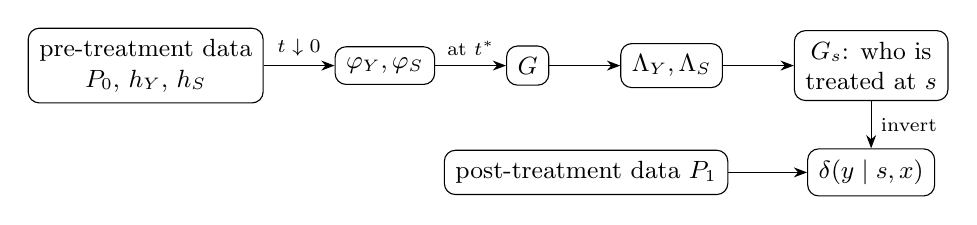
\begin{tikzpicture}[node distance=0.6cm and 0.9cm, box/.style={draw,rounded corners,align=center,font=\small,inner sep=4pt}, >=Stealth]
    \node[box] (pre) {pre-treatment data\\$P_0,\,h_Y,\,h_S$};
    \node[box,right=of pre] (phi) {$\varphi_Y,\varphi_S$};
    \node[box,right=of phi] (G) {$G$};
    \node[box,right=of G] (Lam) {$\Lambda_Y,\Lambda_S$};
    \node[box,right=of Lam] (Gs) {$G_s$: who is\\treated at $s$};
    \node[box,below=of Gs] (delta) {$\delta(y\mid s,x)$};
    \node[box,left=1.0cm of delta] (post) {post-treatment data $P_1$};
    \draw[->] (pre) -- node[above,font=\scriptsize]{$t\downarrow0$} (phi);
    \draw[->] (phi) -- node[above,font=\scriptsize]{at $t^*$} (G);
    \draw[->] (G) -- (Lam);
    \draw[->] (Lam) -- (Gs);
    \draw[->] (Gs) -- node[right,font=\scriptsize]{invert} (delta);
    \draw[->] (post) -- (delta);
  \end{tikzpicture}}

  \raggedright
  \medskip
  \small
  \begin{tabular}{p{0.27\textwidth}p{0.6\textwidth}}
    \toprule
    Assumption & Role \\
    \midrule
    No anticipation & pre-treatment period is a clean competing-risks problem ($\delta$ absent) \\
    Selection only via $(x,V)$ & clocks independent given $V$; treated $=$ risk set reweighted by $V_S$ \\
    MPH separability, $V\perp x$ & index structure $\Lap(\varphi\Lambda)$ behind all three steps \\
    $\E V<\infty$ & step 1 (short-duration hazard ratios) \\
    2-D covariate variation & step 2: trace $\Lap$ on an open set $\Rightarrow$ identifies the dependence \\
    \bottomrule
  \end{tabular}
\note{
\textbf{Use this slide to recap.} If the audience retains one picture, it should be this chain.

Information flows from the pre-treatment data, where nothing causal happens, to the structure of selection. The post-treatment data are then used only once, at the end, to read off $\delta$ after the selection has been removed.

\textbf{What is \emph{not} on the list:} an excluded instrument, selection on observables, parametric functional forms, or multiple spells.
}
\end{frame}

% =====================================================================
\begin{frame}{Heterogeneous effects (Model 1b, Prop.~4)}
  \[
  \theta_Y(t\mid s,x,V)=\begin{cases}\lambda_Y(t)\varphi_Y(x)V_Y & t\le s\\ \lambda_\Delta(t)\varphi_\Delta(x)V_\Delta & t>s\end{cases},
  \qquad (V_Y,V_\Delta,V_S)\sim G_\Delta,
  \]
  \[
  \text{so the effect is}\quad
  \delta(t\mid x,V)=\frac{\lambda_\Delta(t)\varphi_\Delta(x)V_\Delta}{\lambda_Y(t)\varphi_Y(x)V_Y}.
  \]
  \begin{itemize}
    \item \textbf{Gained:} the effect varies with unobservables, and $V_\Delta$ may correlate with $V_S$. This allows \textbf{selection on gains} (Roy-type sorting).
    \item \textbf{Lost:} $\delta$ can no longer depend on the treatment date $s$.
    \item \textbf{Why it works:} after $S$, the residual duration of the treated cohort is again MPH, in $\Lambda_\Delta(y)-\Lambda_\Delta(s)$ with frailty $V_\Delta$, so Elbers--Ridder can be rerun on it.
    \item \textbf{Extra assumptions:} variation in $\varphi_\Delta(x)$, and $\E[V_\Delta V_S]<\infty$. The moment is of the \emph{product} because the treated cohort is tilted by $V_S$.
  \end{itemize}
\note{
\textbf{Why the trade-off arises.} In Model 1a, $\delta(t\mid s,x)$ can be any function, but it is common to all types. Identification inverts $P_1$ for a single unknown function $D$ given a known $G_s$. In Model 1b the post-treatment hazard has its own frailty, so after treatment there is a new unknown distribution (that of $V_\Delta$ in the treated cohort). Identifying it requires running the MPH argument again on post-treatment durations. That argument needs the post-treatment hazard to be proportional and the same function for all $s$, so dependence on $s$ is ruled out.

\textbf{Proof idea (appendix).} Take second derivatives of the data with respect to $(y,s)$. Letting $y,s\downarrow0$ identifies $\varphi_\Delta$ (the analogue of step 1). Then the trivariate Laplace transform is traced on an open set (the analogue of step 2).
}
\end{frame}

% =====================================================================
\begin{frame}{Multiple spells: the within estimator (Model 2c, Prop.~6)}
  Strata (same person twice, siblings, \ldots) with two spells sharing the same unobservables:
  \[ \theta_{Y_k}(t\mid S_k,V)=\lambda_{Y_k}(t)\,V_Y(t)\,\delta_k(t\mid S_k)^{\1\{t>S_k\}},\qquad k=1,2,\quad \lambda_{Y_1}\equiv1. \]
  $V_Y(t)$ may be \textbf{any process common to both spells}, and there is \textbf{no model for $S_k$}.

  \medskip
  Given that the first exit in the stratum happens at $t$, which spell was it? $V_Y(t)$ \textbf{cancels}:
  \[ \Pr(\text{spell 1}\mid t,\text{histories},V)=\frac{\theta_{Y_1}(t)}{\theta_{Y_1}(t)+\theta_{Y_2}(t)}. \]
  \small
  \begin{tabular}{lll}
    \toprule
    treated at $t$ & $\Pr(\text{spell 1 first})$ & identifies \\
    \midrule
    neither & $1/(1+\lambda_{Y_2})$ & $\lambda_{Y_2}$ \\
    spell 1 only & $\delta_1/(\delta_1+\lambda_{Y_2})$ & $\delta_1$ \\
    spell 2 only & $1/(1+\lambda_{Y_2}\delta_2)$ & $\delta_2$ \\
    both & $\delta_1/(\delta_1+\lambda_{Y_2}\delta_2)$ & (overidentifying) \\
    \bottomrule
  \end{tabular}

  \normalsize
  \medskip
  \textbf{Cox partial likelihood $=$ conditional logit $=$ fixed effects.} \textbf{Cost:} $V$ identical across spells, and \textbf{no causal links across spells}.
\note{
\textbf{Why this is the panel analogue.} In linear panels the within transformation removes the individual effect. Here, conditioning on ``one of the two spells ends at $t$'' removes the stratum effect, because it multiplies both hazards. This is Cox's partial-likelihood logic, applied to strata (Holt \& Prentice 1974; Ridder \& Tunal\i{} 1999).

\textbf{What is gained relative to the single-spell case.} No covariates are needed, no finite means, no MPH assumption on how $V$ interacts with time ($V_Y(t)$ can be an arbitrary process), and no model for treatment assignment at all.

\textbf{What it costs.} The unobservable must be \emph{exactly} shared across the two spells. The first spell (or its treatment) must not causally affect the second. For repeated unemployment spells of the same person, that rules out scarring and learning across spells (see the traps discussion on slide 19).

\textbf{Models 2a/2b} (Prop.~5) are MPH versions that also identify $G$; see the appendix.
}
\end{frame}

% =====================================================================
\begin{frame}{What is traded, and critiques}
  \begin{columns}[T]
    \begin{column}{0.45\textwidth}
      \textbf{Not needed}
      \begin{itemize}
        \item an excluded instrument
        \item selection on observables
        \item parametric functional forms
        \item multiple spells (single-spell results)
      \end{itemize}
      \textbf{Needed}
      \begin{itemize}
        \item no anticipation (untestable)
        \item time-invariant unobservables, $V\perp x$
        \item MPH proportionality
        \item 2-D, non-proportional covariate variation
        \item finite means; continuous time
      \end{itemize}
    \end{column}
    \begin{column}{0.53\textwidth}
      \textbf{Critiques}
      \begin{itemize}
        \item Identification comes from $t\downarrow0$, where data are thin. In practice: parametric $\lambda$, discrete $G$ (Heckman--Singer); Monte Carlo evidence in Gaure, R\o ed \& Zhang (2007).
        \item Discrete time: sanction and exit in the same month blur the local signal.
        \item $\delta$ is a hazard ratio \emph{conditional on $V$}. Effects on mean duration or population survival require $G$.
        \item Transitory shocks hitting both hazards (the caseworker reacts to this week's low effort) violate Assn.~2.
      \end{itemize}
    \end{column}
  \end{columns}
\note{
\textbf{One-sentence summary of the trade.} The excluded \emph{variable} is replaced by (i) an excluded timing \emph{shock}, (ii) multiplicative separability, (iii) time-invariant heterogeneity, and (iv) no anticipation.

\textbf{On the last critique.} This is the most common objection in the sanctions literature. Sanctions are typically triggered by observed non-compliance, which may reflect a temporary drop in search effort that also lowers the exit rate. That is a time-varying unobservable affecting both hazards, which Model 1a excludes. Model 2c partly addresses it, but only with multiple spells.
}
\end{frame}

% =====================================================================
\begin{frame}{Connection: staggered adoption DiD}
  \textbf{Same skeleton}
  \begin{itemize}
    \item $Y^*(s)$ $\leftrightarrow$ $Y_t(g)$, potential outcomes indexed by adoption cohort.
    \item No anticipation is \emph{the same assumption} (Callaway \& Sant'Anna 2021; Sun \& Abraham 2021; Borusyak, Jaravel \& Spiess 2024).
    \item The risk set $R_s$ $\leftrightarrow$ the \emph{not-yet-treated} comparison group.
    \item $\delta(t\mid s)$ varies by cohort $s$ and event time $t-s$: the heterogeneity that breaks TWFE.
  \end{itemize}
  \textbf{Differences}
  \begin{itemize}
    \item Selection: \emph{parallel trends} (additive, in levels) vs.\ \emph{time-invariant frailty} (multiplicative, in hazards) plus a random timing shock.
    \item \textbf{Attrition from an absorbing exit:} the treatment changes who remains (slide 13), so ``parallel trends in hazards'' fails \emph{even under random timing}.\\
      DiD on survival probabilities $\to$ a population estimand; ToE $\to$ the individual hazard effect $\delta$, which needs $G$.
    \item If timing is random given observables (\emph{dynamic CIA}), treat later treatment as independent censoring. Population effects on survival are then identified nonparametrically (Fredriksson \& Johansson 2008; Crépon et al.\ 2009; Vikström 2017). ToE is the tool when timing is selected on \emph{unobservables}.
  \end{itemize}
\note{
\textbf{Why the analogy is exact on the skeleton.} Both literatures face a treatment that switches on at a unit-specific date and stays on. Both index potential outcomes by that date. Both impose no anticipation. The comparison ``treated at $s$ vs.\ not yet treated at $s$'' on slide 7 is the event-time-zero comparison of Callaway--Sant'Anna using not-yet-treated controls.

\textbf{Where they part.} In DiD every unit stays in the panel and the outcome is a level. In duration data the outcome is the exit itself, so the sample at risk changes as a \emph{result} of the outcome, and of the treatment. Even if treatment timing were randomly assigned, post-treatment hazard comparisons are contaminated by differential attrition. That is a dynamic-selection bias with no analogue in a balanced panel.

\textbf{Two estimands.} The population effect on survival curves can be obtained by design-based arguments under dynamic CIA. The individual-level hazard effect $\delta$ (needed for structural or behavioural interpretation, e.g.\ search theory) needs a model of $V$.

\textbf{Check citations before the talk.}
}
\end{frame}

% =====================================================================
\begin{frame}{Connection: sequential exogeneity, feedback, and traps}
  \textbf{Sequential exogeneity and feedback}
  \begin{itemize}
    \item A hazard is an intensity relative to the past: $dN_Y(t)-\theta_Y(t\mid\text{past},V)\,dt$ is a martingale difference. This is a continuous-time \emph{sequential moment condition}. No anticipation means treatment is \emph{predetermined}.
    \item In a single absorbing spell, outcome$\to$treatment feedback is degenerate (the only outcome history is ``still here''). The bite is on transitory shocks: $S$ may depend on permanent $V$, not on shocks to the exit rate. This is \emph{strict exogeneity given a fixed effect}.
    \item Model 2c moves toward sequential exogeneity: $S$ is unmodelled and may track a time-varying common $V_Y(t)$, at the cost of needing multiple spells.
  \end{itemize}
  \textbf{Traps: state dependence vs.\ permanent heterogeneity}
  \begin{itemize}
    \item The model separates three objects: $\lambda_Y\downarrow$ (true duration dependence: a trap), $G$ (permanent heterogeneity), and $\delta$ (the effect of an intervention).
    \item Traps suggest \emph{when} you intervene matters: $\delta(t\mid s)$ varying in $s$. Model 1a allows it; Model 1b rules it out.
    \item Multiple-spell results assume no cross-spell effects, i.e.\ they \emph{rule out} lagged duration dependence, the across-spell trap mechanism.
  \end{itemize}
\note{
\textbf{Sequential exogeneity.} In panel data, sequential exogeneity, $\E[u_t\mid x_t,x_{t-1},\ldots,\alpha]=0$, allows future regressors to respond to past outcome shocks (feedback). In counting-process language, the intensity is defined relative to a filtration, and the martingale property is the same type of sequential condition. Treatment history up to $t^-$ can be in the conditioning set, which is exactly no anticipation.

What ToE adds is the fixed effect $V$, together with the assumption that treatment does not respond to transitory shocks that also move the exit hazard. With one spell there is no outcome path to feed back from, except survival itself, so the relevant distinction is permanent vs.\ transitory unobservables. For genuine feedback you need richer outcome histories: multi-state or recurrent events. That leads to the dynamic discrete-choice/treatment literature (Heckman \& Navarro 2007; Abbring \& Heckman 2007, \textit{Handbook of Econometrics} 6B).

\textbf{Traps.} The primer's ``trap or sorting?'' question is the same identification problem as $\lambda$ vs.\ $G$ in the MPH model. Here, as in Heckman's work, it is resolved by proportionality plus short-duration behaviour, or by multiple spells (Honoré 1993). A poverty-trap application would ask whether an intervention's effect depends on how long someone has been poor, which is $s$-dependence of $\delta$. Note the tension: the multiple-spell route, which relaxes the strong single-spell assumptions, assumes away cross-spell scarring, which is one of the main trap channels.

\textbf{Possible extensions to discuss} (my suggestions, not in the paper): ToE with lagged occurrence dependence across spells; ToE estimands vs.\ DiD estimands on the same data; anticipation as an information shock with observed notification dates.
}
\end{frame}

% =====================================================================
\begin{frame}{Takeaways}
  \begin{enumerate}
    \item \textbf{Timing is information.} Treatment acts only after $S$, while unobservables act throughout. Causal effects are \emph{local}; selection is \emph{global}.
    \item \textbf{The pre-treatment period is a competing-risks experiment with no treatment effect in it.} With MPH structure and non-proportional covariate variation, it reveals who is at risk and who gets treated ($G$). Knowing $G$ strips out selection into treatment and selection out of the risk set afterwards.
    \item \textbf{The price.} No anticipation, multiplicative separability, time-invariant heterogeneity, and a timing shock that is excluded from the outcome. Multiple spells buy back generality at the cost of no cross-spell dynamics.
  \end{enumerate}
\note{
Leave time for discussion. Good questions to put to the group:
(1) In your application, is the timing shock plausibly excluded?
(2) Is $\delta$ (a hazard ratio given $V$) the parameter you care about, or a population survival effect?
(3) What would anticipation look like, and do you observe notification dates?
}
\end{frame}

% =====================================================================
\appendix
\begin{frame}{Appendix A: non-identification (Prop.~1) and the job-search example}
  \centering
  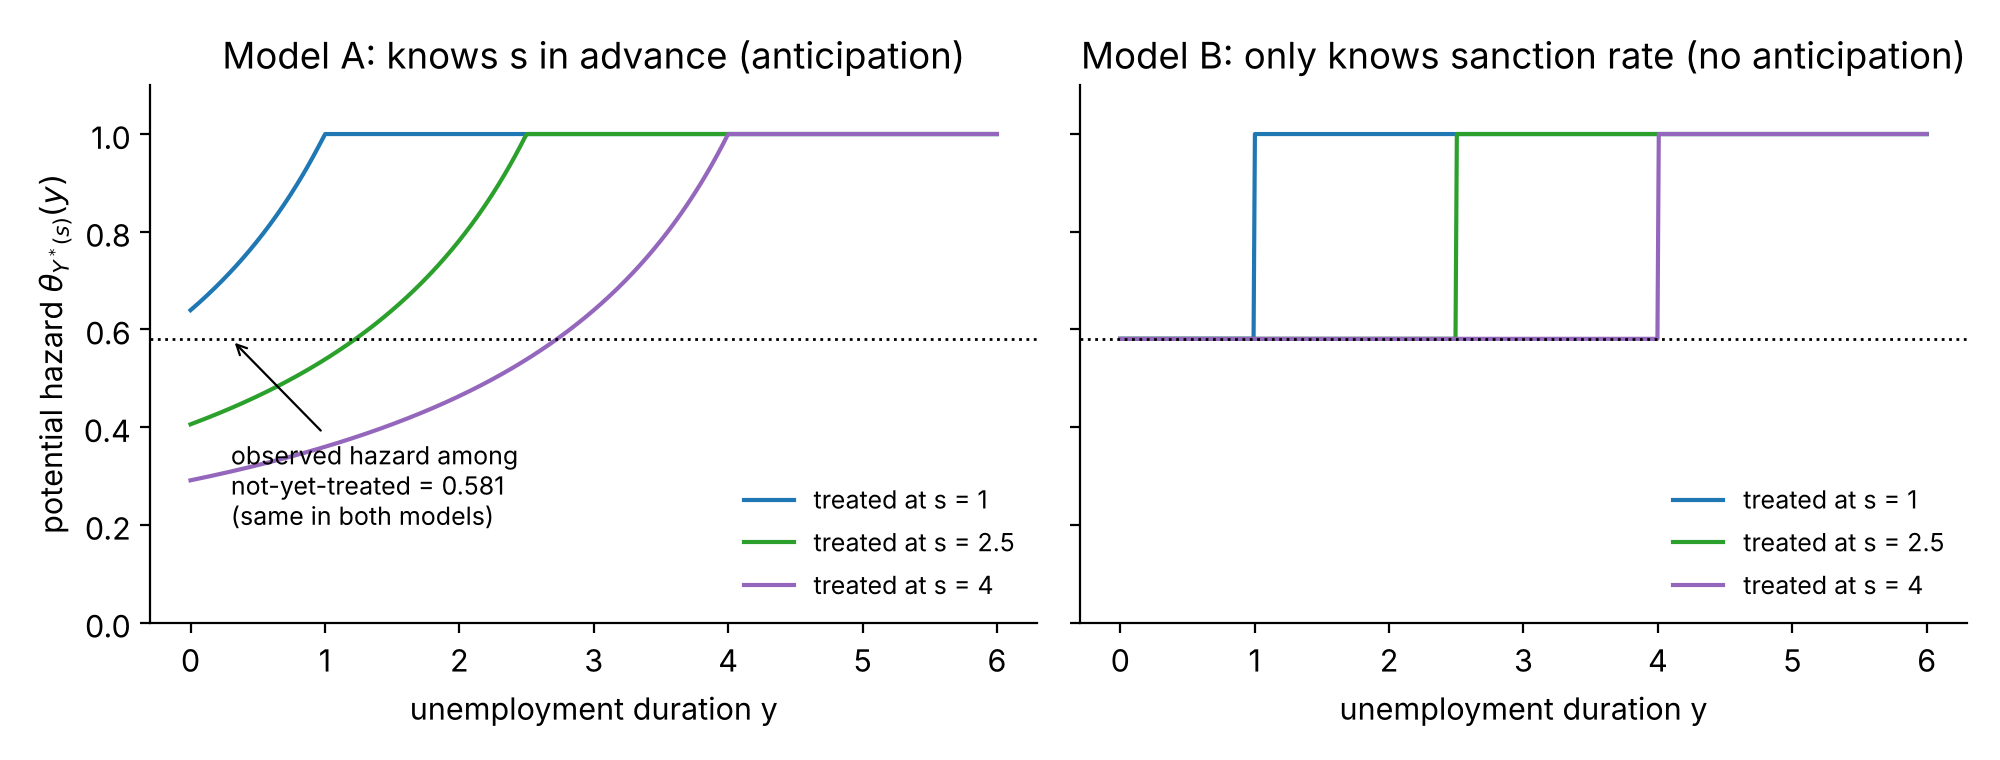
\includegraphics[width=0.82\linewidth]{fig2_anticipation_equivalence.png}

  \raggedright\small
  Model A: the worker knows the sanction date $s$, and search effort (hence the hazard) rises before $s$. Model B: only the sanction rate is known, so the hazard jumps at $s$. With suitably chosen parameters the two produce \emph{identical} data. The data only reveal the hazard among the not-yet-treated (0.581 in both).

  \smallskip
  \textbf{Proof of Prop.~1.} By Tsiatis/Miller there is an independent pair $(\hat Y,\hat S)$ matching the competing-risks part. Use $\hat S$ as the treatment and $\hat Y$'s hazard before treatment for every $Y^*(s)$; define post-treatment hazards from $P_1$.
\note{
Parameters: $w=1$, $b=1/2$. Model A has a discount rate of 5\%; Model B has a discount rate of 1.23\% and a sanction rate of 0.419. Equation (3) of the paper gives Model A's hazard; footnote 11 derives the common observed hazard.
}
\end{frame}

\begin{frame}{Appendix B: data objects vs.\ the paper's $(Q_S,Q_Y)$}
  The paper's data: $Q_S(y,s)=\Pr(Y>y,S>s,Y>S)$ and $Q_Y(y)=\Pr(Y>y,Y<S)$. Then
  \begin{align*}
    P_0(t)&=Q_S(t,t)+Q_Y(t),\\
    h_Y(t)&=-Q_Y'(t)/P_0(t),\qquad h_S(t)=-\partial_sQ_S(t,s)\big|_{s=t}\big/P_0(t),\\
    P_1(y\mid s)&=\partial_sQ_S(y,s)\big/\partial_sQ_S(s,s)\qquad(y>s).
  \end{align*}
  Conversely, $(P_0,h_Y,h_S,P_1)$ determine $(Q_S,Q_Y)$. The objects are equivalent.
\end{frame}

\begin{frame}{Appendix C: uniqueness in step 3}
  Suppose $(a,b)\neq(a',b')$ both satisfy $P_0(t\mid x)=\Lap(\varphi_Y(x)a,\varphi_S(x)b)$ for all $x$. Then $\Lap(pa,qb)=\Lap(pa',qb')$ on an open set of $(p,q)$. By analyticity,
  \[ \Lap(u,v)=\Lap(ku,mv)\quad\text{for all }(u,v)\in(0,\infty)^2,\qquad k=a'/a,\ m=b'/b,\ (k,m)\neq(1,1). \]
  \begin{itemize}
    \item $k,m\ge1$ (or both $\le1$): contradicts $\Lap$ strictly decreasing in each argument (needs $\Pr(V\in(0,\infty)^2)>0$).
    \item $k>1>m$: iterating gives $\Lap(u,v)=\Lap(k^nu,m^nv)\to\Pr(V_Y=0)$ as $n\to\infty$. So $\Lap$ is constant, a contradiction. The case $k<1<m$ is symmetric.
  \end{itemize}
\end{frame}

\begin{frame}{Appendix D: proof sketches for Models 1b, 2a, 2b}
  \small
  \textbf{Model 1b (Prop.~4).} After Prop.~2, for $y>s$:
  \[ \frac{\partial^2Q_S(y,s\mid x)/\partial y\partial s}{\partial^2Q_S(y,s\mid x^*)/\partial y\partial s}\;\xrightarrow{\;y,s\downarrow0\;}\;\varphi_S(x)\varphi_\Delta(x) \quad(\text{needs }\E[V_\Delta V_S]<\infty), \]
  which identifies $\varphi_\Delta$. Then $\partial_sQ_S/(\lambda_S\varphi_S)=\Lap^{(S)}_{G_\Delta}\big(\varphi_Y\Lambda_Y(s),\varphi_\Delta(\Lambda_\Delta(y)-\Lambda_\Delta(s)),\varphi_S\Lambda_S(s)\big)$. Let $s\downarrow0$ to get $\Lambda_\Delta$; vary $x,y$ to trace $\Lap_{G_\Delta}$ on an open set.

  \medskip
  \textbf{Models 2a/2b (Prop.~5).} Two spells per stratum sharing $V=(V_Y,V_S)$ (or $(V_Y,V_\Delta,V_S)$), spell-specific baselines and effects. The two-spell competing-risks structure identifies $\Lambda_{Y_k},\Lambda_{S_k}$ (Abbring \& Van den Berg 2003, JRSSB). The extra cross-spell information then identifies $\delta_k$ and $G$, \textbf{without covariates and without finite means}, mirroring Honoré (1993).
\end{frame}

\end{document}
"
% (or just run ./build.sh)
\documentclass[aspectratio=169,10pt]{beamer}
\ifdefined\withnotes
  \setbeameroption{show notes}
\fi
\setbeamertemplate{navigation symbols}{}
\setbeamertemplate{footline}[frame number]
\setbeamertemplate{note page}{\vspace{1em}\small\insertnote}

\usepackage{amsmath,amssymb,booktabs,tikz}
\usetikzlibrary{arrows.meta,positioning}
\graphicspath{{../figures/}}

\newcommand{\E}{\mathbb{E}}
\newcommand{\1}{\mathbf{1}}
\newcommand{\R}{\mathbb{R}}
\newcommand{\Lap}{\mathcal{L}}
\newcommand{\cov}{\operatorname{Cov}}

\title{The Nonparametric Identification of Treatment Effects in Duration Models}
\subtitle{Abbring \& Van den Berg (2003, \textit{Econometrica})}
\author{Econometrics Reading Group}
\date{}

\begin{document}

% =====================================================================
\begin{frame}
  \titlepage
\note{
\textbf{How to read these notes.} Every slide has a note like this one. The notes say where the slide's content comes from, what the previous slide left unresolved, and what this slide adds. Read slides + notes in order: the argument is cumulative.

\medskip
\textbf{The plan in one sentence.} We want the effect of a treatment that arrives at a random time during a spell. The difficulty is selection on unobservables. The paper's answer is that the \emph{pre-treatment} part of the data is a competing-risks problem; with hazard structure, that part reveals the distribution of unobserved types among those at risk; knowing that distribution lets us strip the selection out of the \emph{post-treatment} part.

\medskip
\textbf{Notation changes relative to the paper.} We write the data as four interpretable objects ($P_0, h_Y, h_S, P_1$) instead of the paper's sub-survival functions $(Q_S,Q_Y)$; the mapping is in the appendix. We write $D(y\mid s,x)$ for the integrated post-treatment hazard (the paper uses $\Upsilon$). We write the bivariate Laplace transform as $\Lap(a,b)$ and its partial derivatives as $\Lap_a,\Lap_b,\Lap_{ab}$.
}
\end{frame}

% =====================================================================
\begin{frame}{The question}
  \textbf{Running example.} An unemployed worker may receive a benefit sanction at a random time $S$ during the spell. Outcome: unemployment duration $Y$.

  \medskip
  \textbf{Target.} The causal effect of the sanction on the \emph{exit rate} to work.

  \medskip
  \textbf{Why this is hard}
  \begin{enumerate}
    \item \textbf{Dynamic treatment:} no fixed treated group; everyone is untreated until $S$.
    \item \textbf{Treatment is censored:} if you find a job before your sanction date, $S$ is never seen.
    \item \textbf{Selection on unobservables:} low-motivation workers get sanctioned earlier \emph{and} exit more slowly.
    \item \textbf{No credible instrument:} whatever shifts sanctions, the worker likely sees and reacts to.
  \end{enumerate}

  \medskip
  \textbf{Punchline.} The \emph{timing} of $S$ relative to $Y$ does the job of the instrument, at the price of structure on hazards.
\note{
Point 4 is the paper's own argument (Section 1) against IV. If a variable affects treatment and the agent can see it, a forward-looking agent adjusts behaviour, so the variable also affects the outcome hazard directly. Exclusion restrictions are therefore hard to defend in dynamic settings.

Point 2 explains why the data are unusual. We see $S$ only for people with $S<Y$. This censoring is not a nuisance to be fixed; it is what turns the pre-treatment data into a competing-risks problem (slide 10).

The punchline is what the rest of the talk earns. Keep the four difficulties visible: each later assumption addresses one of them.
}
\end{frame}

% =====================================================================
\begin{frame}{Primer 1: hazards and dynamic selection}
  \begin{columns}[T]
    \begin{column}{0.47\textwidth}
      \textbf{Hazard} of a duration $T$:
      \[ \theta(t)=\lim_{dt\downarrow0}\tfrac{\Pr(T\in[t,t+dt)\mid T\ge t)}{dt} \]
      $\Lambda(t)=\int_0^t\theta$, \quad $\Pr(T>t)=e^{-\Lambda(t)}$.

      \smallskip
      In every instant, each survivor flips a coin with success probability $\theta(t)\,dt$.

      \medskip
      \textbf{Heterogeneity:} $\theta(t\mid V)=\lambda(t)\,V$. Then the hazard we \emph{observe} is
      \[ \bar\theta(t)=\lambda(t)\;\E[V\mid T\ge t], \]
      and $\E[V\mid T\ge t]$ \textbf{falls}: high-$V$ people leave first.
    \end{column}
    \begin{column}{0.53\textwidth}
      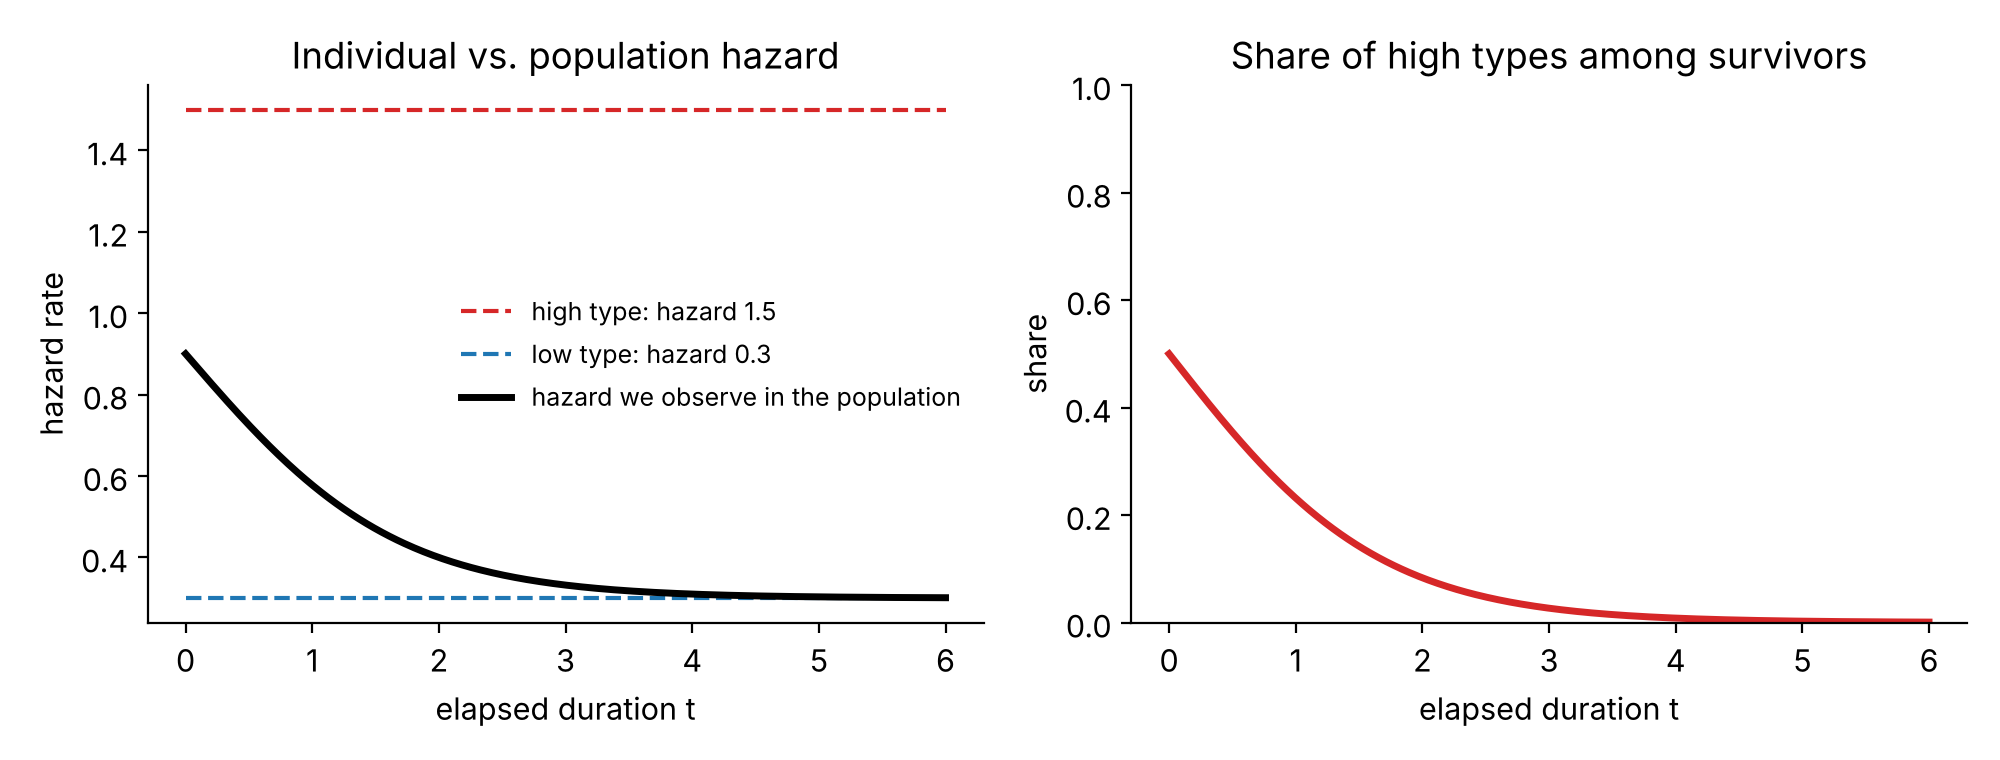
\includegraphics[width=\linewidth]{fig1_dynamic_selection.png}
    \end{column}
  \end{columns}

  \medskip
  \textbf{Trap or sorting?} A falling exit rate can be true duration dependence ($\lambda\downarrow$) or composition ($\E[V\mid T\ge t]\downarrow$). This is Heckman's \emph{true vs.\ spurious state dependence}, in continuous time.
\note{
\textbf{Derivation of the observed hazard.} The survival function is $\Pr(T>t)=\E[e^{-V\Lambda(t)}]$, with $\Lambda(t)=\int_0^t \lambda$. The population hazard is $-\frac{d}{dt}\log\Pr(T>t)=\lambda(t)\,\E[Ve^{-V\Lambda(t)}]/\E[e^{-V\Lambda(t)}]$. The ratio is the mean of $V$ under weights $e^{-V\Lambda(t)}$, i.e.\ $\E[V\mid T\ge t]$. The weight $e^{-V\Lambda(t)}$ is the probability that a type-$V$ person is still there. That is the whole idea of dynamic selection.

\textbf{Why it matters for treatment effects.} The people still unemployed and untreated at month 6 are a selected group. Comparing ``treated at month 6'' with ``not yet treated at month 6'' is only valid if we know how both groups were selected up to month 6. Every identification step below is about learning that selection.

\textbf{Figure.} Two types with \emph{constant} hazards 0.3 and 1.5 produce a population hazard that falls from 0.9 to 0.3. Nobody's hazard changes; only the composition does.

\textbf{The coin-flip view} matters later. Conditional on the hazard, the moment of the event is pure chance. This is the source of the ``randomization'' the paper exploits (footnote 15).
}
\end{frame}

% =====================================================================
\begin{frame}{Primer 2: the MPH model and the Laplace-transform toolkit}
  \textbf{Mixed proportional hazard:} $\theta(t\mid x,V)=\lambda(t)\,\varphi(x)\,V$, \quad $V\sim G$, \ $V\perp x$. Then
  \[ \Pr(T>t\mid x)=\E\big[e^{-V\varphi(x)\Lambda(t)}\big]=\Lap\big(\varphi(x)\Lambda(t)\big),\qquad \Lap(a):=\E[e^{-aV}]. \]
  \textbf{Toolkit.} $e^{-aV}$ is the probability that type $V$ survives to index $a$. So derivatives of $\log\Lap$ are \emph{moments among survivors}. In two dimensions, $\Lap(a,b)=\E[e^{-aV_Y-bV_S}]$:
  \[
    -\partial_a\log\Lap=\E[V_Y\mid\text{surv.}],\qquad
    -\partial_b\log\Lap=\E[V_S\mid\text{surv.}],\qquad
    \partial^2_{ab}\log\Lap=\cov(V_Y,V_S\mid\text{surv.}).
  \]
  \textbf{Single-risk identification (Elbers \& Ridder 1982), in 3 steps}
  \begin{enumerate}
    \item $t\downarrow0$: nobody has been selected out yet, so hazard ratios across $x$ give $\varphi(x)$ (needs $\E V<\infty$).
    \item At $t^*$ with $\Lambda(t^*)=1$: $\Pr(T>t^*\mid x)=\Lap(\varphi(x))$. Varying $x$ traces $\Lap$, hence $G$.
    \item Any $t$: solve $\Pr(T>t\mid x)=\Lap(\varphi(x)\Lambda(t))$ for $\Lambda(t)$.
  \end{enumerate}
  \textbf{We will run exactly this logic in two dimensions.}
\note{
\textbf{Where the toolkit comes from.} $\log\Lap(a,b)$ is the cumulant generating function of $(-V_Y,-V_S)$, evaluated under tilting by $e^{-aV_Y-bV_S}$. First derivative: $\partial_a\log\Lap=-\E[V_Ye^{-aV_Y-bV_S}]/\Lap=-\E_w[V_Y]$. Differentiate again in $b$: $\partial_b(-\E_w[V_Y])=\E_w[V_YV_S]-\E_w[V_Y]\E_w[V_S]=\cov_w(V_Y,V_S)$. The weights $w$ are survival probabilities, so ``$\E_w$'' means ``among survivors''. Two consequences we use repeatedly:
(i) the observed hazard is $\lambda\varphi\times(-\partial_a\log\Lap)$;
(ii) the dependence between $V_Y$ and $V_S$ among survivors (the selection) is a cross-derivative.

\textbf{Step 1 in detail.} The hazard is $\lambda(t)\varphi(x)\E[V\mid T\ge t,x]$. As $t\downarrow0$, $\E[V\mid T\ge t,x]\to\E[V]$, which is finite by assumption and the same for all $x$ because $V\perp x$. The ratio across $x$ and $x^*$ therefore tends to $\varphi(x)/\varphi(x^*)=\varphi(x)$. Note that identification uses the behaviour of short durations, where data are thin (critique on slide 17).

\textbf{Step 2.} The normalization $\Lambda(t^*)=1$ fixes the scale. Once $\varphi$ is known, $x\mapsto\Pr(T>t^*\mid x)$ is $\Lap$ evaluated at known points. Varying $x$ traces $\Lap$ on an interval. Laplace transforms are analytic, so $\Lap$ is then pinned down everywhere, and it determines $G$ uniquely.

\textbf{Step 3.} $\Lap$ is strictly decreasing, so invert.
}
\end{frame}

% =====================================================================
\begin{frame}{Set-up: potential outcomes indexed by treatment time}
  \begin{itemize}
    \item Treatments are dates $s\in[0,\infty]$ ($s=\infty$: never). Potential outcomes $Y^*(s)$; observed $Y=Y^*(S)$.
    \item \textbf{No anticipation:} $\theta_{Y^*(s)}(t)=\theta_{Y^*(s')}(t)$ for $t\le\min(s,s')$. A future treatment date does not affect today's hazard.\\
      Reacting to the sanction \emph{regime} is allowed (it is in every $Y^*(s)$), so the effect is \emph{``treated at $s$ vs.\ later, under this regime''}.
  \end{itemize}
  \begin{center}
  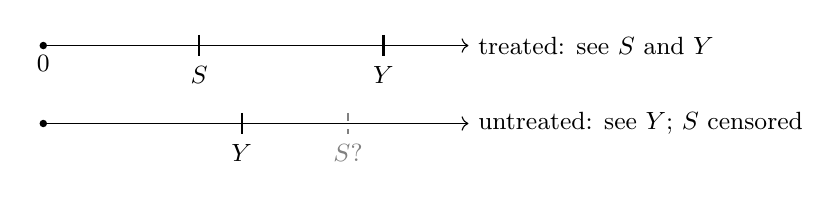
\begin{tikzpicture}[scale=0.9]
    \draw[->] (0,0) -- (6,0) node[right] {\small treated: see $S$ and $Y$};
    \fill (0,0) circle (1.5pt) node[below] {\small 0};
    \draw[thick] (2.2,0.15) -- (2.2,-0.15) node[below] {\small $S$};
    \draw[thick] (4.8,0.15) -- (4.8,-0.15) node[below] {\small $Y$};
    \draw[->] (0,-1.1) -- (6,-1.1) node[right] {\small untreated: see $Y$; $S$ censored};
    \fill (0,-1.1) circle (1.5pt);
    \draw[thick] (2.8,-0.95) -- (2.8,-1.25) node[below] {\small $Y$};
    \draw[dashed,gray] (4.3,-0.95) -- (4.3,-1.25) node[below] {\small $S$?};
  \end{tikzpicture}
  \end{center}
  \textbf{What the data reveal} (all conditional on $x$):
  \begin{itemize}
    \item $P_0(t)=\Pr(Y>t,S>t)$: nothing has happened by $t$;
    \item $h_Y(t)$, $h_S(t)$: rate of exiting untreated / of being treated, among those with nothing yet;
    \item $P_1(y\mid s)=\Pr(Y>y\mid S=s,\,Y>s)$: post-treatment survival of the \textbf{cohort treated at $s$}.
  \end{itemize}
  \textbf{Fact (Prop.~1):} any such data can be rationalized with no anticipation \emph{and} random assignment. So no anticipation is untestable, and we need a model of selection.
\note{
\textbf{Why index potential outcomes by a date.} A dynamically assigned binary treatment is really a continuum of mutually exclusive treatments, ``treated at $s$''. This is exactly the staggered-adoption set-up, where potential outcomes are indexed by the adoption cohort $g$ (slide 18).

\textbf{No anticipation.} The paper states it for integrated hazards; hazard paths agreeing up to $\min(s,s')$ is the same thing. In biostatistics this is a mild consistency condition. In economics it is behavioural: if a worker knows the sanction date and searches harder beforehand, it fails. If information arrives before treatment, the paper suggests treating the \emph{information shock} as the treatment.

\textbf{The data objects.} These four objects are equivalent to the paper's $(Q_S,Q_Y)$; see the appendix. The pre-treatment objects ($P_0,h_Y,h_S$) are classic \emph{competing-risks} data: two things can happen and we see which happens first. $P_1$ is the only place where the treatment effect can appear.

\textbf{Proposition 1 (de-emphasized).} By the Tsiatis/Miller result, any competing-risks data are generated by some \emph{independent} pair of latent durations. Use that pair for the pre-treatment part, and define the post-treatment hazard to match $P_1$. The result is a model with random assignment and no anticipation that fits the data perfectly. Two lessons: selection cannot be told from causality without structure, and anticipation cannot be detected. The paper's job-search illustration is in the appendix.
}
\end{frame}

% =====================================================================
\begin{frame}{The model}
  \textbf{Assumption 2 (selection on $(x,V)$):} $Y^*(\cdot)\perp S \mid (x,V)$, with $V$ time-invariant.

  \medskip
  \textbf{Model 1a.}
  \[
  \theta_Y(t\mid s,x,V)=\lambda_Y(t)\,\varphi_Y(x)\,V_Y\cdot\delta(t\mid s,x)^{\1\{t>s\}},\qquad
  \theta_S(t\mid x,V)=\lambda_S(t)\,\varphi_S(x)\,V_S,
  \]
  with $(V_Y,V_S)\sim G$ \textbf{arbitrarily dependent}, independent of $x$.

  \medskip
  \begin{itemize}
    \item Two MPH hazards. Their link through $\cov(V_Y,V_S)$ is the \textbf{selection on unobservables}.
    \item $\delta$ is the \textbf{causal effect}: a hazard multiplier after treatment. It may vary with $t$, $s$ (hence with $t-s$) and $x$, but not with $V$.
    \item No anticipation is built in: $\delta$ only acts for $t>s$.
    \item The same $x$ enters both hazards, so there is \textbf{no exclusion restriction}. $\lambda$'s, $\varphi$'s, $G$, $\delta$ are all nonparametric.
  \end{itemize}

  \medskip
  \textbf{Assn.~3:} $\{(\varphi_Y(x),\varphi_S(x))\}$ contains an open set of $\R^2$. \quad \textbf{Assn.~4:} $\E V_Y,\E V_S<\infty$.\\
  Normalizations: $\varphi(x^*)=1$, $\Lambda(t^*)=1$.
\note{
\textbf{How the model emerges from the set-up.} No anticipation says pre-treatment hazards do not depend on $s$. Assumption 2 says all dependence between $Y$ and $S$ runs through $(x,V)$. Together they imply: conditional on $(x,V)$, $Y$ and $S$ are linked \emph{only} through the causal factor $\delta$. That is why $\delta$ can be called a treatment effect.

\textbf{Why hazard-based assignment matters.} $S$ is modelled by a hazard, not by a threshold-crossing rule. So even conditional on $(x,V)$, $S$ is random: $\varphi_S(x)V_S\Lambda_S(S)$ is a unit exponential independent of $(x,V)$. This random component moves $S$ around without affecting $Y$ except through treatment. It is the analogue of an instrument (slide 8).

\textbf{Assumption 3 is not an exclusion restriction, but it is not free.} The covariates must move the two hazards \emph{non-proportionally}. With $\varphi_j(x)=e^{x'\beta_j}$ you need at least two continuous covariates and $(\beta_Y\ \beta_S)$ of full rank.

\textbf{Allowed but not shown:} mass points of $V$ at zero (never treated / never exit). Also $\Pr(Y=S)=0$ (continuous time, no ties).
}
\end{frame}

% =====================================================================
\begin{frame}{The selection problem at the moment of treatment}
  Fix a duration $s$. Write $a_s=\varphi_Y(x)\Lambda_Y(s)$, $b_s=\varphi_S(x)\Lambda_S(s)$.

  \medskip
  \textbf{Who is still at risk} (nothing happened by $s$):\quad $dG_{R_s}(v)\propto e^{-a_s v_Y-b_s v_S}\,dG(v)$.\\[2pt]
  \textbf{Who is treated at $s$:} the risk set, reweighted by the treatment intensity, \quad $dG_{s}(v)\propto v_S\,dG_{R_s}(v)$.

  \medskip
  \textbf{Exit hazards right at $s$:}
  \[
  \underbrace{\lambda_Y(s)\varphi_Y(x)\,\E_{R_s}[V_Y]}_{\text{not yet treated}}
  \qquad\text{vs.}\qquad
  \underbrace{\lambda_Y(s)\varphi_Y(x)\,\delta(s\mid s,x)\,\E_{s}[V_Y]}_{\text{just treated}}
  \]
  \[
  \frac{\text{just treated}}{\text{not yet treated}}
  \;=\;\delta(s\mid s,x)\times\underbrace{\Big(1+\frac{\cov_{R_s}(V_Y,V_S)}{\E_{R_s}[V_Y]\,\E_{R_s}[V_S]}\Big)}_{\text{selection factor}}
  \]
  \begin{itemize}
    \item If $V_Y\perp V_S$ among survivors, timing is as good as random at $s$: the ratio \emph{is} the causal effect.
    \item Otherwise we need the \textbf{joint distribution of types among survivors}. The pre-treatment data will supply it.
  \end{itemize}
\note{
\textbf{This slide is the heart of the paper's logic.} It reduces the selection problem to one object.

\textbf{Derivation.} Being at risk at $s$ means $Y>s$ and $S>s$. Given $V$, no anticipation means $Y$'s hazard before $s$ is the untreated one, so the probability of being at risk is $e^{-a_sV_Y}e^{-b_sV_S}$ (Assumption 2 lets the two terms multiply). By Bayes' rule, the type distribution in the risk set is $G$ reweighted by that probability. Among those at risk, the chance of being treated in $[s,s+ds)$ is $\lambda_S(s)\varphi_S(x)V_S\,ds$. So the treated cohort is the risk set reweighted by $V_S$.

The mean of $V_Y$ in the treated cohort is
$\E_s[V_Y]=\E_{R_s}[V_YV_S]/\E_{R_s}[V_S]=\E_{R_s}[V_Y]+\cov_{R_s}(V_Y,V_S)/\E_{R_s}[V_S]$.
Divide by $\E_{R_s}[V_Y]$ to get the selection factor.

\textbf{Reading it.} Suppose low-motivation people (low $V_Y$) are sanctioned more (high $V_S$), so the covariance is negative. Then the just-treated have low $V_Y$, and the naive comparison \emph{understates} a positive effect of sanctions on exit. This is the classic ``Heckman selection'' structure, with a control-function-like correction factor.

\textbf{The ratio on the left is data.} The hazard of the just-treated is $-\partial_y\log P_1(y\mid s)$ as $y\downarrow s$; the hazard of the not-yet-treated is $h_Y(s)$. So everything hinges on the selection factor, a feature of the joint distribution of $(V_Y,V_S)$ among those at risk at $s$.
}
\end{frame}

% =====================================================================
\begin{frame}{Timing as an instrument}
  \footnotesize
  \begin{tabular}{p{0.2\textwidth}p{0.29\textwidth}p{0.41\textwidth}}
    \toprule
    & Static selection / IV & Timing of events \\
    \midrule
    Exogenous variation in treatment
    & excluded variable $Z$
    & the timing shock: given $(x,V)$, $S=\Lambda_S^{-1}\!\big(\tfrac{E_S}{\varphi_S(x)V_S}\big)$, $E_S\sim\text{Exp}(1)$ \\[3pt]
    What is excluded from the outcome
    & the \emph{variable} $Z$
    & the \emph{shock} $E_S$ (via Assn.~2) \\[3pt]
    Correcting for who selects in
    & control function $\E[U\mid D=1,Z]$
    & selection factor / $G_s$, from the competing-risks data \\[3pt]
    Covariate requirement
    & $Z$ shifts $D$, not $Y$
    & $x$ shifts both hazards, \emph{non-proportionally} (Assn.~3) \\
    \bottomrule
  \end{tabular}

  \normalsize
  \bigskip
  \textbf{Why timing is informative.} The treatment acts only \emph{after} $S$; $V$ acts \emph{throughout}.
  \begin{itemize}
    \item Causal effect $\Rightarrow$ \textbf{local} dependence: exits bunch right after $S$, \emph{whenever} $S$ occurs.
    \item Selection $\Rightarrow$ \textbf{global} dependence: early-treated people are early leavers in general.
  \end{itemize}
  In a static latent-index model the treatment effect needs an exclusion restriction. Here the timing replaces it.
\note{
\textbf{The point of the table.} An IV design needs two things: (i) variation in treatment that is unrelated to the outcome's unobservables, and (ii) a way to handle the fact that the people who take treatment are selected.

(i) In a static threshold model $D=\1\{\mu(Z)>U\}$, treatment is deterministic given $(Z,U)$, so exogenous variation must come from an excluded $Z$. With hazard-based assignment, treatment \emph{timing} is still random given $(x,V)$. The representation uses the fact that $\varphi_S(x)V_S\Lambda_S(S)$ is unit exponential. The exclusion restriction has not disappeared: it moved from an observed variable to an unobserved shock. Assumption 2 says the timing shock $E_S$ is independent of everything that drives $Y$. Be candid about this in the talk.

(ii) The selection correction is the analogue of a control function. Here it is not estimated from an excluded instrument; it comes from the competing-risks part of the data (next three slides).

\textbf{Local vs.\ global.} This is the paper's own intuition (Section 3.2) and the basis of the companion paper on testing the sign of $\delta$. The figure on the next slide makes it concrete.
}
\end{frame}

% =====================================================================
\begin{frame}{What the data look like}
  \centering
  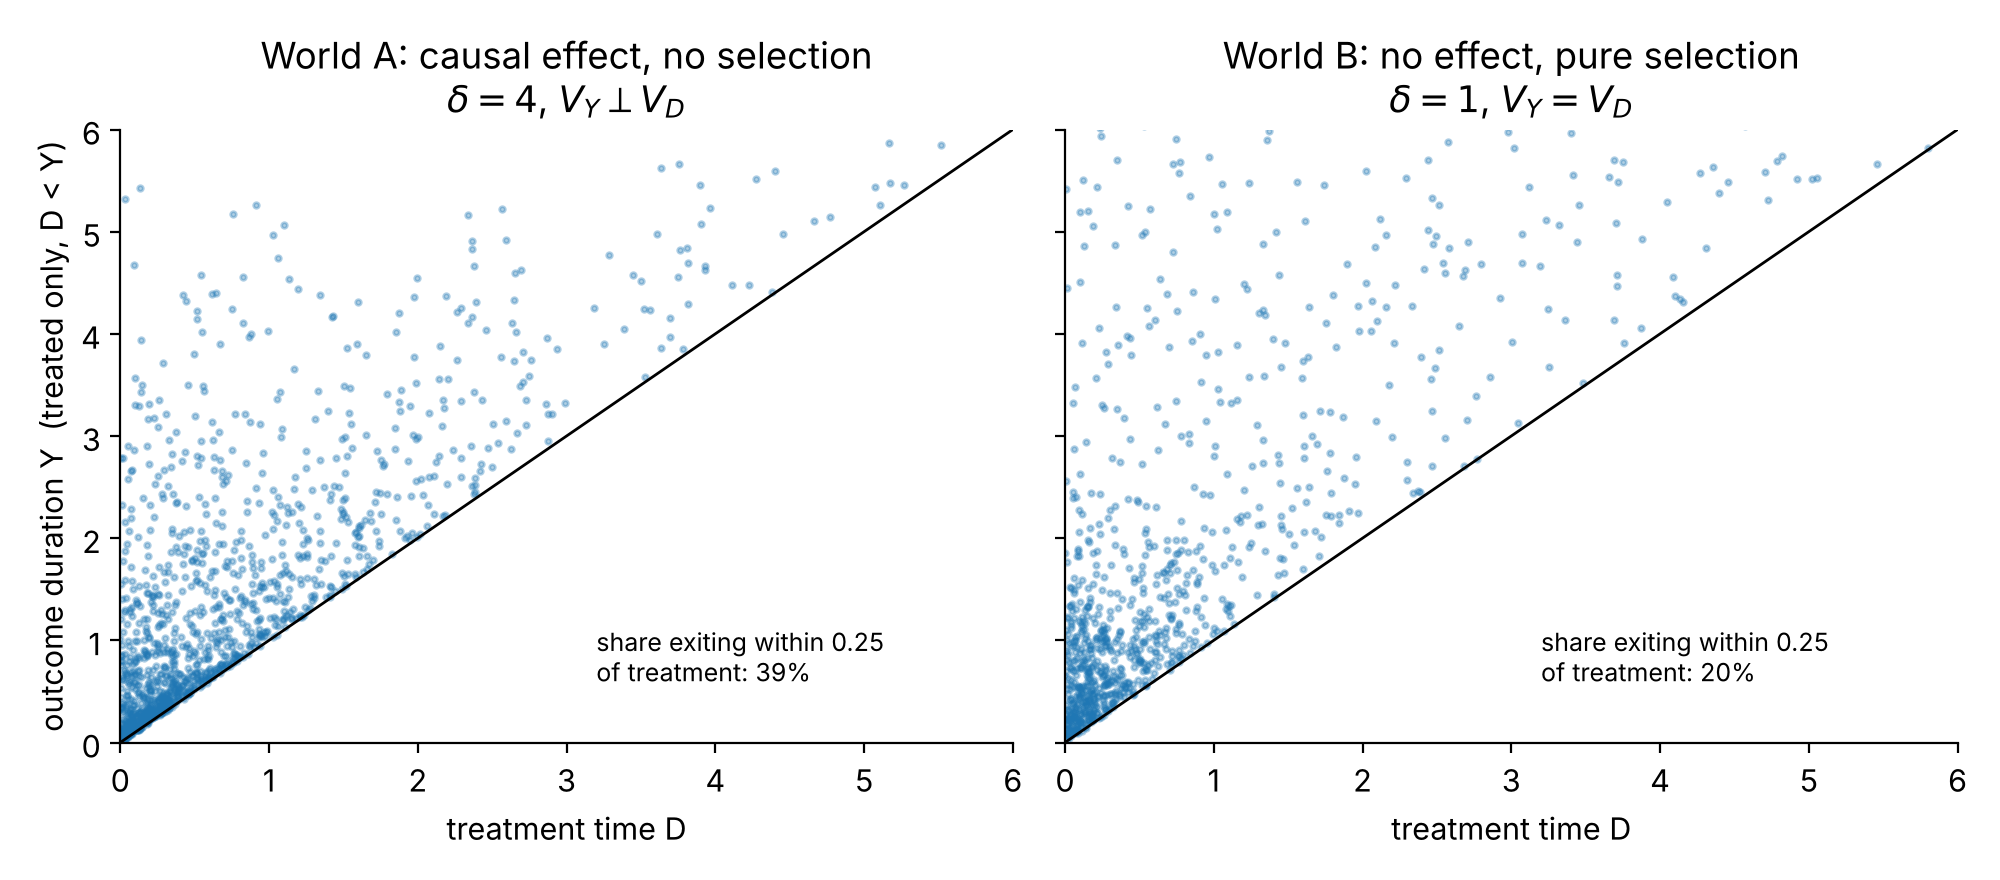
\includegraphics[width=0.85\linewidth]{fig3_local_vs_global.png}

  \raggedright\small
  Treated observations only. Left: $\delta=4$, independent frailties. Right: $\delta=1$, $V_Y=V_S$. A causal effect makes points hug the diagonal \emph{at every $S$}. Selection produces quick exits only where high types are concentrated (small $S$).
\note{
\textbf{Simulation.} Two types (0.25 and 2), constant baseline hazards. World A: types for $Y$ and $S$ drawn independently, and treatment multiplies the exit hazard by 4. World B: one common type, no effect.

Both worlds show a positive association between $S$ and $Y$, and in both some people exit quickly after treatment. The difference is \emph{where} the quick exits are. In A they occur after treatment at any $S$; in B they are concentrated at small $S$, where the high types still are. The formal argument quantifies exactly this: how many quick post-treatment exits would we expect from selection alone, given the types at risk at $s$?

Script: \texttt{figures/make\_figures.py}.
}
\end{frame}

% =====================================================================
\begin{frame}{The pre-treatment data are a competing-risks problem}
  Before treatment there are two latent clocks: $Y^0$ (exit if never treated) and $S$. Their joint survival is
  \[ \Pr(Y^0>y,\,S>s\mid x)=\Lap\big(\varphi_Y(x)\Lambda_Y(y),\;\varphi_S(x)\Lambda_S(s)\big). \qquad \text{($\delta$ does not appear!)}\]
  We only see the \emph{first} event: the diagonal $y=s=t$, i.e.\ $P_0(t\mid x)=\Lap(a_t(x),b_t(x))$, plus which event it was.

  \smallskip
  \textbf{Tsiatis (1975):} without structure, any such data are generated by \emph{independent} clocks. The dependence, i.e.\ the selection, is unidentified.

  \begin{center}
    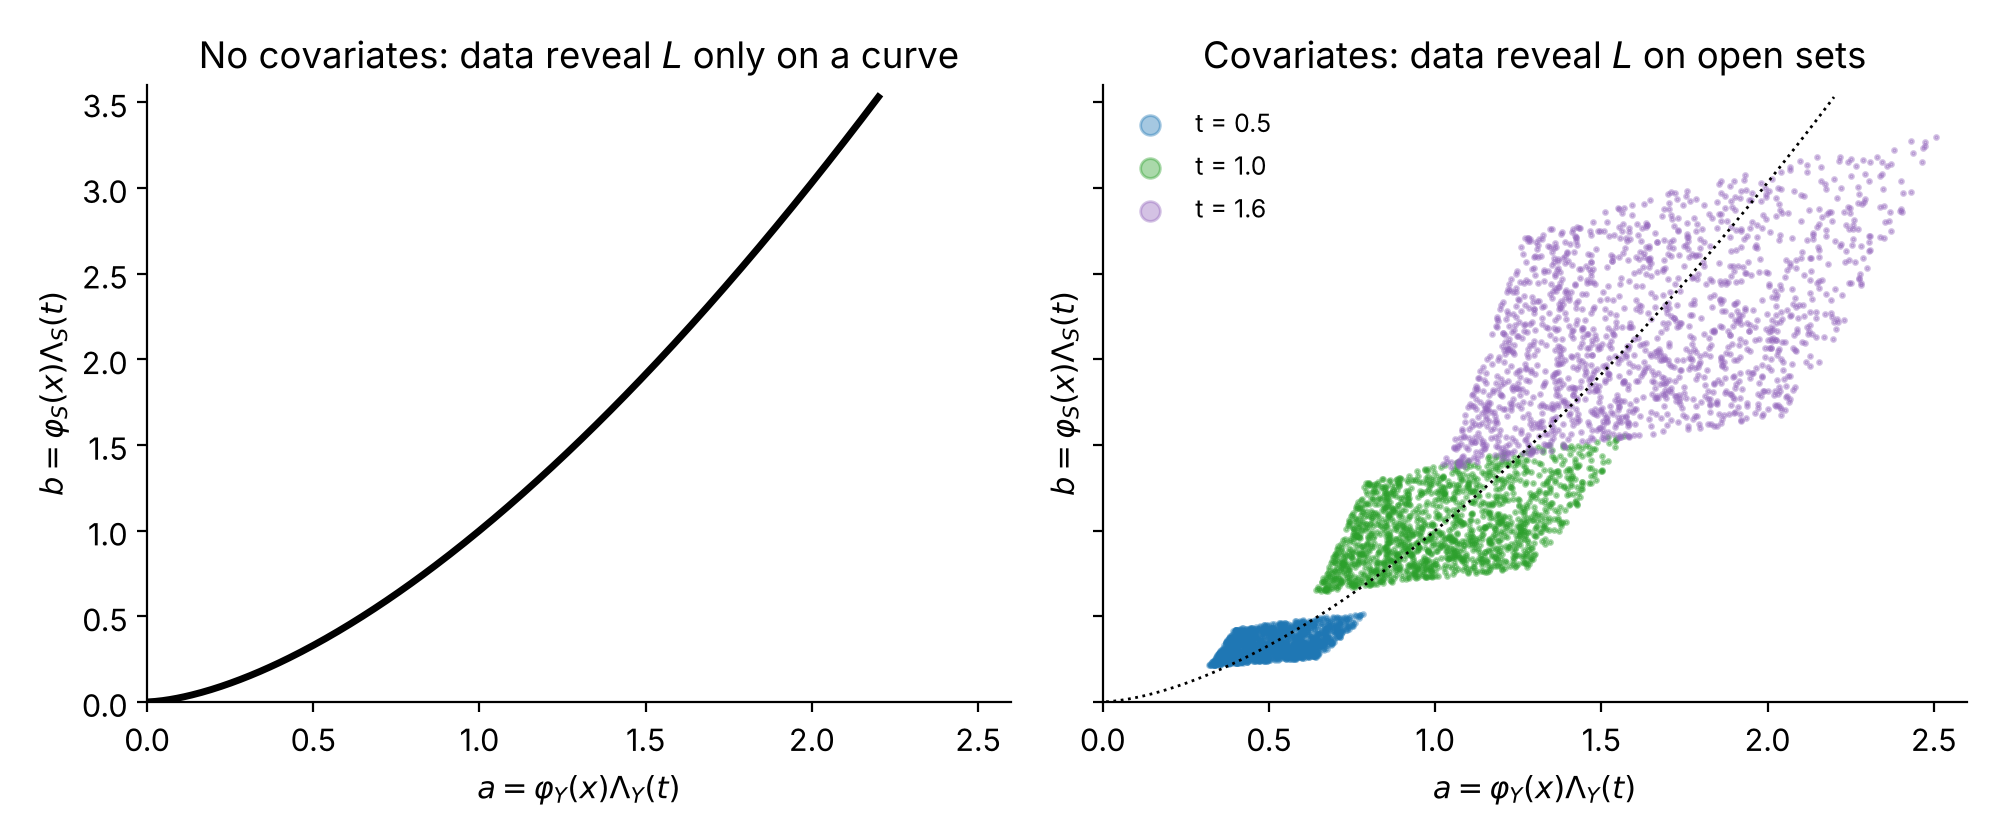
\includegraphics[width=0.56\linewidth]{fig4_competing_risks_geometry.png}
  \end{center}
  \vspace{-6pt}
  \small Without $x$, the data reveal $\Lap$ only along a curve $t\mapsto(\Lambda_Y(t),\Lambda_S(t))$. A curve cannot pin down a function of two variables. With $x$ shifting the two hazards separately, the data reveal $\Lap$ on \emph{open sets}.
\note{
\textbf{Why this is the crucial step.} Slide 7 showed that everything hinges on the joint distribution of $(V_Y,V_S)$. The only place to learn it without using the outcome we want to explain is the pre-treatment period. There, by no anticipation, nothing causal is going on. We just watch two clocks race.

\textbf{The joint survival.} Given $V$, the two clocks are independent with integrated hazards $\varphi_Y\Lambda_YV_Y$ and $\varphi_S\Lambda_SV_S$. Integrating over $G$ gives the bivariate Laplace transform evaluated at the two indices.

\textbf{Geometry of non-identification.} With no covariates, data at duration $t$ tell us $\Lap$ at one point $(\Lambda_Y(t),\Lambda_S(t))$. As $t$ varies we learn $\Lap$ along a curve, plus the slopes of $\Lap$ in the two directions along that curve (from the cause-specific hazards). Many bivariate distributions agree on those values, including independent ones. That is Tsiatis' result.

\textbf{How covariates break it.} At a fixed $t$, varying $x$ moves the point to $(\varphi_Y(x)\Lambda_Y(t),\varphi_S(x)\Lambda_S(t))$. If the two $\varphi$'s move independently (Assumption 3), the point sweeps out a two-dimensional patch. Knowing an analytic function on any open patch determines it everywhere. This is why Assumption 3 must be two-dimensional, and it is what makes the selection identified.
}
\end{frame}

% =====================================================================
\begin{frame}{Identifying the competing-risks part (Prop.~2): three steps}
  \textbf{Step 1: $\varphi$'s from short durations} (nobody has been selected out yet):
  \[ \frac{h_Y(t\mid x)}{h_Y(t\mid x^*)}=\frac{\varphi_Y(x)\,\E[V_Y\mid R_t,x]}{\E[V_Y\mid R_t,x^*]}\;\xrightarrow{\;t\downarrow0\;}\;\varphi_Y(x),\qquad\text{same for }\varphi_S. \]
  Uses \emph{which} event happened and $\E V<\infty$.

  \medskip
  \textbf{Step 2: $G$ at the normalization date} ($\Lambda_Y(t^*)=\Lambda_S(t^*)=1$):
  \[ P_0(t^*\mid x)=\Lap\big(\varphi_Y(x),\varphi_S(x)\big). \]
  Known points fill an open set (Assn.~3), so $\Lap$ is known there. $\Lap$ is real-analytic, so it is known on $(0,\infty)^2$, and $\Lap$ determines $G$, \textbf{including the dependence between $V_Y$ and $V_S$}.

  \medskip
  \textbf{Step 3: baselines.} For every $t$, $(\Lambda_Y(t),\Lambda_S(t))$ is the unique $(a,b)$ with
  \[ P_0(t\mid x)=\Lap\big(\varphi_Y(x)\,a,\;\varphi_S(x)\,b\big)\quad\text{for all }x. \]

  \medskip
  $\Rightarrow$ $\lambda_Y,\lambda_S,\varphi_Y,\varphi_S,G$ are identified \textbf{without touching post-treatment data}.
\note{
\textbf{Relation to the paper.} The paper proves Proposition 2 by citing Abbring \& Van den Berg (2003, JRSSB). The three steps here are a self-contained route that makes the logic visible. It is Elbers--Ridder (slide 4) in two dimensions.

\textbf{Step 1.} The cause-specific hazard of exiting untreated among those at risk is $h_Y(t\mid x)=\lambda_Y(t)\varphi_Y(x)\E[V_Y\mid R_t,x]=\lambda_Y(t)\varphi_Y(x)\big(-\partial_a\log\Lap\big)(a_t,b_t)$. As $t\downarrow0$ the risk set is the whole population. Because $V\perp x$ and $\E V_Y<\infty$, the conditional mean tends to the same constant for all $x$, and $\lambda_Y(t)$ cancels in the ratio.

\textbf{Step 2.} Only the probability of ``no event yet'' is needed here; the cause-specific information was used in step 1. Analyticity: $\Lap(a,b)=\E e^{-aV_Y-bV_S}$ is real-analytic on $(0,\infty)^2$, and two analytic functions that agree on an open set agree on the whole connected domain. A distribution on $[0,\infty)^2$ is determined by its Laplace transform.

\textbf{Step 3.} Uniqueness is proved in the appendix. Idea: if two pairs fit, then $\Lap(u,v)=\Lap(ku,mv)$ for some $(k,m)\neq(1,1)$. Iterating forces $\Lap$ to be constant, which contradicts it being strictly decreasing.

\textbf{What is used where.} No anticipation: the pre-treatment hazard of $Y$ is the untreated one, so $\delta$ is absent. Assumption 2: the clocks are independent given $V$. MPH: the index structure. Assumption 4: step 1. Assumption 3: step 2.
}
\end{frame}

% =====================================================================
\begin{frame}{Where the selection shows up in the data}
  From the toolkit, applied to the observed $P_0(t\mid x)=\Lap(a_t(x),b_t(x))$:
  \[ \frac{\partial^2\log P_0}{\partial a\,\partial b}=\cov\big(V_Y,V_S\mid \text{nothing happened by }t,\,x\big). \]
  \begin{itemize}
    \item $V_Y\perp V_S$ $\iff$ $\Lap(a,b)=\Lap_Y(a)\Lap_S(b)$ $\iff$ $\log P_0$ is \textbf{additively separable} in the two covariate indices.
    \item Selection on unobservables $=$ an \textbf{interaction}: a covariate that raises the treatment hazard changes how the exit index affects survival.
    \item Seeing an interaction requires the two indices to move separately (Assn.~3). That is where the instrument-like requirement hides: \emph{no exclusion, but non-proportional covariate effects}.
  \end{itemize}

  \medskip
  The selection factor of slide 7 is then a function of identified objects:
  \[ 1+\frac{\cov_{R_s}(V_Y,V_S)}{\E_{R_s}V_Y\;\E_{R_s}V_S}=\frac{\Lap\,\Lap_{ab}}{\Lap_a\,\Lap_b}\Big|_{(a_s,b_s)}
  \quad\Rightarrow\quad
  \delta(s\mid s,x)=\frac{\text{observed hazard ratio at }s}{\Lap\Lap_{ab}/(\Lap_a\Lap_b)}. \]
\note{
\textbf{This answers ``how does competing risks identify the selection''.} The covariance of unobserved types among survivors is a cross-partial of the log probability that nothing has happened yet, taken with respect to the two covariate indices.

\textbf{Intuition.} Suppose $x_1$ mainly raises the treatment hazard and $x_2$ mainly raises the exit hazard. With independent types, their effects on $\log P_0$ add up. With correlated types, raising treatment intensity removes (through treatment) people whose exit propensity is also unusual. This changes the composition of who remains, and so changes the marginal effect of $x_2$ on survival. That interaction is the fingerprint of selection.

\textbf{Algebra for the selection factor.} $\E_{R_s}V_Y=-\Lap_a/\Lap$, $\E_{R_s}V_S=-\Lap_b/\Lap$, and $\E_{R_s}[V_YV_S]=\Lap_{ab}/\Lap$. Hence $\E_{R_s}[V_YV_S]/(\E V_Y\E V_S)=\Lap\Lap_{ab}/(\Lap_a\Lap_b)$, which equals $1+\cov/(\E\E)$. With independent types this is exactly 1.

\textbf{Caveat.} In practice, functional form ($\varphi=e^{x'\beta}$, parametric $\lambda$, discrete $G$) does much of the work that the open-set argument does in theory.
}
\end{frame}

% =====================================================================
\begin{frame}{Stripping out selection after treatment (Prop.~3)}
  For $y>s$, with $D(y\mid s,x)=\int_s^y\lambda_Y(\tau)\delta(\tau\mid s,x)\,d\tau$ the integrated post-treatment hazard,
  \[
  P_1(y\mid s,x)=\E_{G_s}\!\Big[e^{-\varphi_Y(x)V_Y\,D(y\mid s,x)}\Big]
  =\frac{\Lap_b\big(a_s+\varphi_Y(x)D(y\mid s,x),\;b_s\big)}{\Lap_b(a_s,b_s)}.
  \]
  \begin{itemize}
    \item The left side is data. On the right, everything except $D$ is known from Prop.~2.
    \item The right side is strictly decreasing in $D$, so \textbf{invert} to get $D(y\mid s,x)$. Then $\delta(y\mid s,x)=\partial_yD/\lambda_Y(y)$.
  \end{itemize}

  \medskip
  \textbf{Two selection problems, both solved by knowing $G$:}
  \begin{enumerate}
    \item \textbf{Selection into treatment at $s$:} the $V_S$-tilt of $G_s$ (absent if $V_Y\perp V_S$).
    \item \textbf{Selection out after $s$:} the treated cohort's survivors drift toward low $V_Y$. This happens whenever $V_Y$ varies, \emph{even with random timing}. So hazard ratios at longer horizons $\neq\delta$.
  \end{enumerate}
\note{
\textbf{Derivation (this is the paper's eq.~(10), normalized).} Given $V$, the density of being treated at $s$ while still unemployed is $\lambda_S(s)\varphi_S V_S\,e^{-b_sV_S}e^{-a_sV_Y}$. Survival from $s$ to $y$ after treatment is $e^{-\varphi_YV_YD(y\mid s)}$. Multiply, integrate over $G$, and divide by the same expression with $y=s$:
$P_1=\E[V_Se^{-(a_s+\varphi_YD)V_Y-b_sV_S}]/\E[V_Se^{-a_sV_Y-b_sV_S}]$.
Since $\Lap_b=-\E[V_Se^{-aV_Y-bV_S}]$, this is the displayed ratio. The paper's (10) is the numerator: $\partial Q_S(y,s)/\partial s=\varphi_S\lambda_S(s)\Lap_b(\ldots)$.

\textbf{Monotonicity.} $\partial_a\Lap_b=\E[V_YV_Se^{\cdots}]>0$, so $\Lap_b$ (which is negative) increases toward 0 as $D$ grows. The ratio therefore falls strictly with $D$.

\textbf{Point 2 is where the duration setting departs from standard treatment-effect intuition.} Suppose timing is random ($V_Y\perp V_S$). The treated cohort starts with the same types as the controls, but if $\delta>1$ its high-$V_Y$ members leave faster. After a while the surviving treated are a more negatively selected group than the surviving controls. A naive hazard ratio at horizon $y-s$ then underestimates $\delta$. Epidemiology knows this as ``the hazards of hazard ratios'' (Hern\'an 2010). The model handles it because $G$ is known.

\textbf{Slide 7 is the special case $y\downarrow s$} of this slide.
}
\end{frame}

% =====================================================================
\begin{frame}{The identification chain, and where each assumption is used}
  \centering
  \resizebox{\linewidth}{!}{%
  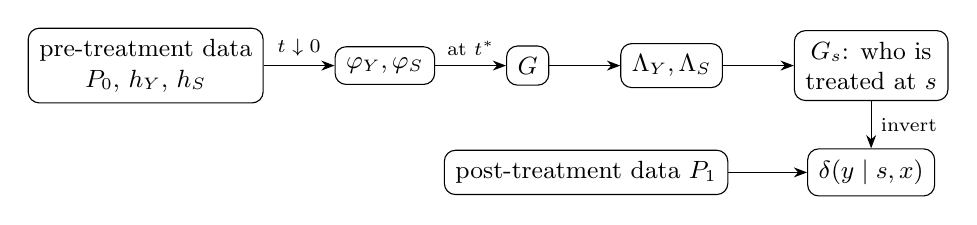
\begin{tikzpicture}[node distance=0.6cm and 0.9cm, box/.style={draw,rounded corners,align=center,font=\small,inner sep=4pt}, >=Stealth]
    \node[box] (pre) {pre-treatment data\\$P_0,\,h_Y,\,h_S$};
    \node[box,right=of pre] (phi) {$\varphi_Y,\varphi_S$};
    \node[box,right=of phi] (G) {$G$};
    \node[box,right=of G] (Lam) {$\Lambda_Y,\Lambda_S$};
    \node[box,right=of Lam] (Gs) {$G_s$: who is\\treated at $s$};
    \node[box,below=of Gs] (delta) {$\delta(y\mid s,x)$};
    \node[box,left=1.0cm of delta] (post) {post-treatment data $P_1$};
    \draw[->] (pre) -- node[above,font=\scriptsize]{$t\downarrow0$} (phi);
    \draw[->] (phi) -- node[above,font=\scriptsize]{at $t^*$} (G);
    \draw[->] (G) -- (Lam);
    \draw[->] (Lam) -- (Gs);
    \draw[->] (Gs) -- node[right,font=\scriptsize]{invert} (delta);
    \draw[->] (post) -- (delta);
  \end{tikzpicture}}

  \raggedright
  \medskip
  \small
  \begin{tabular}{p{0.27\textwidth}p{0.6\textwidth}}
    \toprule
    Assumption & Role \\
    \midrule
    No anticipation & pre-treatment period is a clean competing-risks problem ($\delta$ absent) \\
    Selection only via $(x,V)$ & clocks independent given $V$; treated $=$ risk set reweighted by $V_S$ \\
    MPH separability, $V\perp x$ & index structure $\Lap(\varphi\Lambda)$ behind all three steps \\
    $\E V<\infty$ & step 1 (short-duration hazard ratios) \\
    2-D covariate variation & step 2: trace $\Lap$ on an open set $\Rightarrow$ identifies the dependence \\
    \bottomrule
  \end{tabular}
\note{
\textbf{Use this slide to recap.} If the audience retains one picture, it should be this chain.

Information flows from the pre-treatment data, where nothing causal happens, to the structure of selection. The post-treatment data are then used only once, at the end, to read off $\delta$ after the selection has been removed.

\textbf{What is \emph{not} on the list:} an excluded instrument, selection on observables, parametric functional forms, or multiple spells.
}
\end{frame}

% =====================================================================
\begin{frame}{Heterogeneous effects (Model 1b, Prop.~4)}
  \[
  \theta_Y(t\mid s,x,V)=\begin{cases}\lambda_Y(t)\varphi_Y(x)V_Y & t\le s\\ \lambda_\Delta(t)\varphi_\Delta(x)V_\Delta & t>s\end{cases},
  \qquad (V_Y,V_\Delta,V_S)\sim G_\Delta,
  \]
  \[
  \text{so the effect is}\quad
  \delta(t\mid x,V)=\frac{\lambda_\Delta(t)\varphi_\Delta(x)V_\Delta}{\lambda_Y(t)\varphi_Y(x)V_Y}.
  \]
  \begin{itemize}
    \item \textbf{Gained:} the effect varies with unobservables, and $V_\Delta$ may correlate with $V_S$. This allows \textbf{selection on gains} (Roy-type sorting).
    \item \textbf{Lost:} $\delta$ can no longer depend on the treatment date $s$.
    \item \textbf{Why it works:} after $S$, the residual duration of the treated cohort is again MPH, in $\Lambda_\Delta(y)-\Lambda_\Delta(s)$ with frailty $V_\Delta$, so Elbers--Ridder can be rerun on it.
    \item \textbf{Extra assumptions:} variation in $\varphi_\Delta(x)$, and $\E[V_\Delta V_S]<\infty$. The moment is of the \emph{product} because the treated cohort is tilted by $V_S$.
  \end{itemize}
\note{
\textbf{Why the trade-off arises.} In Model 1a, $\delta(t\mid s,x)$ can be any function, but it is common to all types. Identification inverts $P_1$ for a single unknown function $D$ given a known $G_s$. In Model 1b the post-treatment hazard has its own frailty, so after treatment there is a new unknown distribution (that of $V_\Delta$ in the treated cohort). Identifying it requires running the MPH argument again on post-treatment durations. That argument needs the post-treatment hazard to be proportional and the same function for all $s$, so dependence on $s$ is ruled out.

\textbf{Proof idea (appendix).} Take second derivatives of the data with respect to $(y,s)$. Letting $y,s\downarrow0$ identifies $\varphi_\Delta$ (the analogue of step 1). Then the trivariate Laplace transform is traced on an open set (the analogue of step 2).
}
\end{frame}

% =====================================================================
\begin{frame}{Multiple spells: the within estimator (Model 2c, Prop.~6)}
  Strata (same person twice, siblings, \ldots) with two spells sharing the same unobservables:
  \[ \theta_{Y_k}(t\mid S_k,V)=\lambda_{Y_k}(t)\,V_Y(t)\,\delta_k(t\mid S_k)^{\1\{t>S_k\}},\qquad k=1,2,\quad \lambda_{Y_1}\equiv1. \]
  $V_Y(t)$ may be \textbf{any process common to both spells}, and there is \textbf{no model for $S_k$}.

  \medskip
  Given that the first exit in the stratum happens at $t$, which spell was it? $V_Y(t)$ \textbf{cancels}:
  \[ \Pr(\text{spell 1}\mid t,\text{histories},V)=\frac{\theta_{Y_1}(t)}{\theta_{Y_1}(t)+\theta_{Y_2}(t)}. \]
  \small
  \begin{tabular}{lll}
    \toprule
    treated at $t$ & $\Pr(\text{spell 1 first})$ & identifies \\
    \midrule
    neither & $1/(1+\lambda_{Y_2})$ & $\lambda_{Y_2}$ \\
    spell 1 only & $\delta_1/(\delta_1+\lambda_{Y_2})$ & $\delta_1$ \\
    spell 2 only & $1/(1+\lambda_{Y_2}\delta_2)$ & $\delta_2$ \\
    both & $\delta_1/(\delta_1+\lambda_{Y_2}\delta_2)$ & (overidentifying) \\
    \bottomrule
  \end{tabular}

  \normalsize
  \medskip
  \textbf{Cox partial likelihood $=$ conditional logit $=$ fixed effects.} \textbf{Cost:} $V$ identical across spells, and \textbf{no causal links across spells}.
\note{
\textbf{Why this is the panel analogue.} In linear panels the within transformation removes the individual effect. Here, conditioning on ``one of the two spells ends at $t$'' removes the stratum effect, because it multiplies both hazards. This is Cox's partial-likelihood logic, applied to strata (Holt \& Prentice 1974; Ridder \& Tunal\i{} 1999).

\textbf{What is gained relative to the single-spell case.} No covariates are needed, no finite means, no MPH assumption on how $V$ interacts with time ($V_Y(t)$ can be an arbitrary process), and no model for treatment assignment at all.

\textbf{What it costs.} The unobservable must be \emph{exactly} shared across the two spells. The first spell (or its treatment) must not causally affect the second. For repeated unemployment spells of the same person, that rules out scarring and learning across spells (see the traps discussion on slide 19).

\textbf{Models 2a/2b} (Prop.~5) are MPH versions that also identify $G$; see the appendix.
}
\end{frame}

% =====================================================================
\begin{frame}{What is traded, and critiques}
  \begin{columns}[T]
    \begin{column}{0.45\textwidth}
      \textbf{Not needed}
      \begin{itemize}
        \item an excluded instrument
        \item selection on observables
        \item parametric functional forms
        \item multiple spells (single-spell results)
      \end{itemize}
      \textbf{Needed}
      \begin{itemize}
        \item no anticipation (untestable)
        \item time-invariant unobservables, $V\perp x$
        \item MPH proportionality
        \item 2-D, non-proportional covariate variation
        \item finite means; continuous time
      \end{itemize}
    \end{column}
    \begin{column}{0.53\textwidth}
      \textbf{Critiques}
      \begin{itemize}
        \item Identification comes from $t\downarrow0$, where data are thin. In practice: parametric $\lambda$, discrete $G$ (Heckman--Singer); Monte Carlo evidence in Gaure, R\o ed \& Zhang (2007).
        \item Discrete time: sanction and exit in the same month blur the local signal.
        \item $\delta$ is a hazard ratio \emph{conditional on $V$}. Effects on mean duration or population survival require $G$.
        \item Transitory shocks hitting both hazards (the caseworker reacts to this week's low effort) violate Assn.~2.
      \end{itemize}
    \end{column}
  \end{columns}
\note{
\textbf{One-sentence summary of the trade.} The excluded \emph{variable} is replaced by (i) an excluded timing \emph{shock}, (ii) multiplicative separability, (iii) time-invariant heterogeneity, and (iv) no anticipation.

\textbf{On the last critique.} This is the most common objection in the sanctions literature. Sanctions are typically triggered by observed non-compliance, which may reflect a temporary drop in search effort that also lowers the exit rate. That is a time-varying unobservable affecting both hazards, which Model 1a excludes. Model 2c partly addresses it, but only with multiple spells.
}
\end{frame}

% =====================================================================
\begin{frame}{Connection: staggered adoption DiD}
  \textbf{Same skeleton}
  \begin{itemize}
    \item $Y^*(s)$ $\leftrightarrow$ $Y_t(g)$, potential outcomes indexed by adoption cohort.
    \item No anticipation is \emph{the same assumption} (Callaway \& Sant'Anna 2021; Sun \& Abraham 2021; Borusyak, Jaravel \& Spiess 2024).
    \item The risk set $R_s$ $\leftrightarrow$ the \emph{not-yet-treated} comparison group.
    \item $\delta(t\mid s)$ varies by cohort $s$ and event time $t-s$: the heterogeneity that breaks TWFE.
  \end{itemize}
  \textbf{Differences}
  \begin{itemize}
    \item Selection: \emph{parallel trends} (additive, in levels) vs.\ \emph{time-invariant frailty} (multiplicative, in hazards) plus a random timing shock.
    \item \textbf{Attrition from an absorbing exit:} the treatment changes who remains (slide 13), so ``parallel trends in hazards'' fails \emph{even under random timing}.\\
      DiD on survival probabilities $\to$ a population estimand; ToE $\to$ the individual hazard effect $\delta$, which needs $G$.
    \item If timing is random given observables (\emph{dynamic CIA}), treat later treatment as independent censoring. Population effects on survival are then identified nonparametrically (Fredriksson \& Johansson 2008; Crépon et al.\ 2009; Vikström 2017). ToE is the tool when timing is selected on \emph{unobservables}.
  \end{itemize}
\note{
\textbf{Why the analogy is exact on the skeleton.} Both literatures face a treatment that switches on at a unit-specific date and stays on. Both index potential outcomes by that date. Both impose no anticipation. The comparison ``treated at $s$ vs.\ not yet treated at $s$'' on slide 7 is the event-time-zero comparison of Callaway--Sant'Anna using not-yet-treated controls.

\textbf{Where they part.} In DiD every unit stays in the panel and the outcome is a level. In duration data the outcome is the exit itself, so the sample at risk changes as a \emph{result} of the outcome, and of the treatment. Even if treatment timing were randomly assigned, post-treatment hazard comparisons are contaminated by differential attrition. That is a dynamic-selection bias with no analogue in a balanced panel.

\textbf{Two estimands.} The population effect on survival curves can be obtained by design-based arguments under dynamic CIA. The individual-level hazard effect $\delta$ (needed for structural or behavioural interpretation, e.g.\ search theory) needs a model of $V$.

\textbf{Check citations before the talk.}
}
\end{frame}

% =====================================================================
\begin{frame}{Connection: sequential exogeneity, feedback, and traps}
  \textbf{Sequential exogeneity and feedback}
  \begin{itemize}
    \item A hazard is an intensity relative to the past: $dN_Y(t)-\theta_Y(t\mid\text{past},V)\,dt$ is a martingale difference. This is a continuous-time \emph{sequential moment condition}. No anticipation means treatment is \emph{predetermined}.
    \item In a single absorbing spell, outcome$\to$treatment feedback is degenerate (the only outcome history is ``still here''). The bite is on transitory shocks: $S$ may depend on permanent $V$, not on shocks to the exit rate. This is \emph{strict exogeneity given a fixed effect}.
    \item Model 2c moves toward sequential exogeneity: $S$ is unmodelled and may track a time-varying common $V_Y(t)$, at the cost of needing multiple spells.
  \end{itemize}
  \textbf{Traps: state dependence vs.\ permanent heterogeneity}
  \begin{itemize}
    \item The model separates three objects: $\lambda_Y\downarrow$ (true duration dependence: a trap), $G$ (permanent heterogeneity), and $\delta$ (the effect of an intervention).
    \item Traps suggest \emph{when} you intervene matters: $\delta(t\mid s)$ varying in $s$. Model 1a allows it; Model 1b rules it out.
    \item Multiple-spell results assume no cross-spell effects, i.e.\ they \emph{rule out} lagged duration dependence, the across-spell trap mechanism.
  \end{itemize}
\note{
\textbf{Sequential exogeneity.} In panel data, sequential exogeneity, $\E[u_t\mid x_t,x_{t-1},\ldots,\alpha]=0$, allows future regressors to respond to past outcome shocks (feedback). In counting-process language, the intensity is defined relative to a filtration, and the martingale property is the same type of sequential condition. Treatment history up to $t^-$ can be in the conditioning set, which is exactly no anticipation.

What ToE adds is the fixed effect $V$, together with the assumption that treatment does not respond to transitory shocks that also move the exit hazard. With one spell there is no outcome path to feed back from, except survival itself, so the relevant distinction is permanent vs.\ transitory unobservables. For genuine feedback you need richer outcome histories: multi-state or recurrent events. That leads to the dynamic discrete-choice/treatment literature (Heckman \& Navarro 2007; Abbring \& Heckman 2007, \textit{Handbook of Econometrics} 6B).

\textbf{Traps.} The primer's ``trap or sorting?'' question is the same identification problem as $\lambda$ vs.\ $G$ in the MPH model. Here, as in Heckman's work, it is resolved by proportionality plus short-duration behaviour, or by multiple spells (Honoré 1993). A poverty-trap application would ask whether an intervention's effect depends on how long someone has been poor, which is $s$-dependence of $\delta$. Note the tension: the multiple-spell route, which relaxes the strong single-spell assumptions, assumes away cross-spell scarring, which is one of the main trap channels.

\textbf{Possible extensions to discuss} (my suggestions, not in the paper): ToE with lagged occurrence dependence across spells; ToE estimands vs.\ DiD estimands on the same data; anticipation as an information shock with observed notification dates.
}
\end{frame}

% =====================================================================
\begin{frame}{Takeaways}
  \begin{enumerate}
    \item \textbf{Timing is information.} Treatment acts only after $S$, while unobservables act throughout. Causal effects are \emph{local}; selection is \emph{global}.
    \item \textbf{The pre-treatment period is a competing-risks experiment with no treatment effect in it.} With MPH structure and non-proportional covariate variation, it reveals who is at risk and who gets treated ($G$). Knowing $G$ strips out selection into treatment and selection out of the risk set afterwards.
    \item \textbf{The price.} No anticipation, multiplicative separability, time-invariant heterogeneity, and a timing shock that is excluded from the outcome. Multiple spells buy back generality at the cost of no cross-spell dynamics.
  \end{enumerate}
\note{
Leave time for discussion. Good questions to put to the group:
(1) In your application, is the timing shock plausibly excluded?
(2) Is $\delta$ (a hazard ratio given $V$) the parameter you care about, or a population survival effect?
(3) What would anticipation look like, and do you observe notification dates?
}
\end{frame}

% =====================================================================
\appendix
\begin{frame}{Appendix A: non-identification (Prop.~1) and the job-search example}
  \centering
  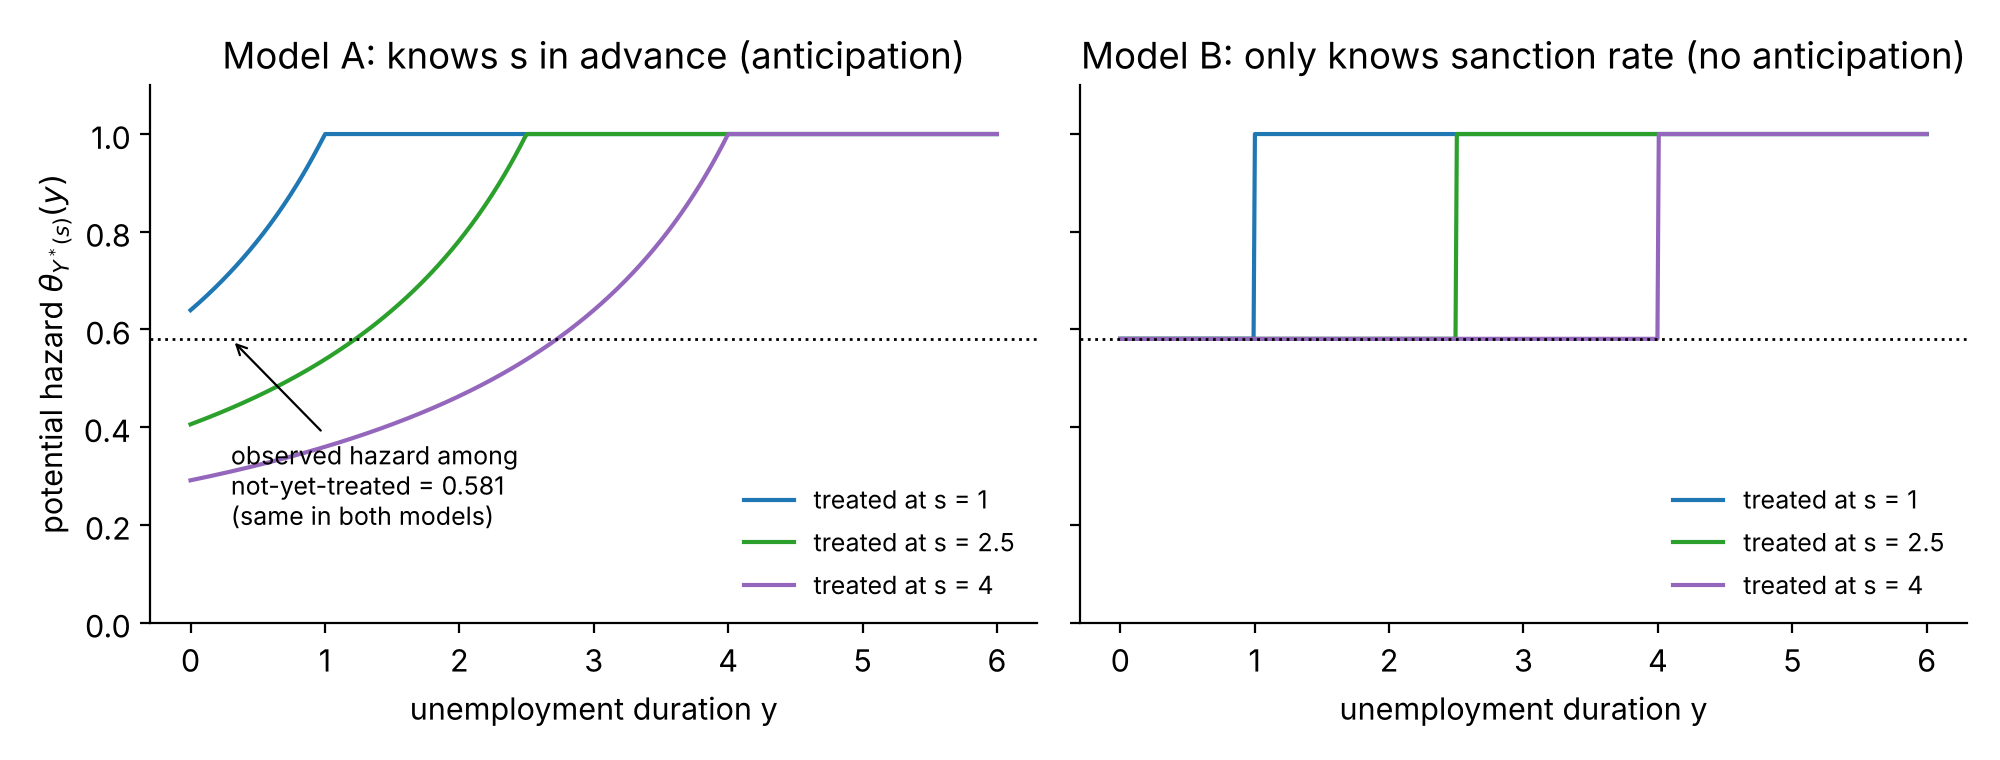
\includegraphics[width=0.82\linewidth]{fig2_anticipation_equivalence.png}

  \raggedright\small
  Model A: the worker knows the sanction date $s$, and search effort (hence the hazard) rises before $s$. Model B: only the sanction rate is known, so the hazard jumps at $s$. With suitably chosen parameters the two produce \emph{identical} data. The data only reveal the hazard among the not-yet-treated (0.581 in both).

  \smallskip
  \textbf{Proof of Prop.~1.} By Tsiatis/Miller there is an independent pair $(\hat Y,\hat S)$ matching the competing-risks part. Use $\hat S$ as the treatment and $\hat Y$'s hazard before treatment for every $Y^*(s)$; define post-treatment hazards from $P_1$.
\note{
Parameters: $w=1$, $b=1/2$. Model A has a discount rate of 5\%; Model B has a discount rate of 1.23\% and a sanction rate of 0.419. Equation (3) of the paper gives Model A's hazard; footnote 11 derives the common observed hazard.
}
\end{frame}

\begin{frame}{Appendix B: data objects vs.\ the paper's $(Q_S,Q_Y)$}
  The paper's data: $Q_S(y,s)=\Pr(Y>y,S>s,Y>S)$ and $Q_Y(y)=\Pr(Y>y,Y<S)$. Then
  \begin{align*}
    P_0(t)&=Q_S(t,t)+Q_Y(t),\\
    h_Y(t)&=-Q_Y'(t)/P_0(t),\qquad h_S(t)=-\partial_sQ_S(t,s)\big|_{s=t}\big/P_0(t),\\
    P_1(y\mid s)&=\partial_sQ_S(y,s)\big/\partial_sQ_S(s,s)\qquad(y>s).
  \end{align*}
  Conversely, $(P_0,h_Y,h_S,P_1)$ determine $(Q_S,Q_Y)$. The objects are equivalent.
\end{frame}

\begin{frame}{Appendix C: uniqueness in step 3}
  Suppose $(a,b)\neq(a',b')$ both satisfy $P_0(t\mid x)=\Lap(\varphi_Y(x)a,\varphi_S(x)b)$ for all $x$. Then $\Lap(pa,qb)=\Lap(pa',qb')$ on an open set of $(p,q)$. By analyticity,
  \[ \Lap(u,v)=\Lap(ku,mv)\quad\text{for all }(u,v)\in(0,\infty)^2,\qquad k=a'/a,\ m=b'/b,\ (k,m)\neq(1,1). \]
  \begin{itemize}
    \item $k,m\ge1$ (or both $\le1$): contradicts $\Lap$ strictly decreasing in each argument (needs $\Pr(V\in(0,\infty)^2)>0$).
    \item $k>1>m$: iterating gives $\Lap(u,v)=\Lap(k^nu,m^nv)\to\Pr(V_Y=0)$ as $n\to\infty$. So $\Lap$ is constant, a contradiction. The case $k<1<m$ is symmetric.
  \end{itemize}
\end{frame}

\begin{frame}{Appendix D: proof sketches for Models 1b, 2a, 2b}
  \small
  \textbf{Model 1b (Prop.~4).} After Prop.~2, for $y>s$:
  \[ \frac{\partial^2Q_S(y,s\mid x)/\partial y\partial s}{\partial^2Q_S(y,s\mid x^*)/\partial y\partial s}\;\xrightarrow{\;y,s\downarrow0\;}\;\varphi_S(x)\varphi_\Delta(x) \quad(\text{needs }\E[V_\Delta V_S]<\infty), \]
  which identifies $\varphi_\Delta$. Then $\partial_sQ_S/(\lambda_S\varphi_S)=\Lap^{(S)}_{G_\Delta}\big(\varphi_Y\Lambda_Y(s),\varphi_\Delta(\Lambda_\Delta(y)-\Lambda_\Delta(s)),\varphi_S\Lambda_S(s)\big)$. Let $s\downarrow0$ to get $\Lambda_\Delta$; vary $x,y$ to trace $\Lap_{G_\Delta}$ on an open set.

  \medskip
  \textbf{Models 2a/2b (Prop.~5).} Two spells per stratum sharing $V=(V_Y,V_S)$ (or $(V_Y,V_\Delta,V_S)$), spell-specific baselines and effects. The two-spell competing-risks structure identifies $\Lambda_{Y_k},\Lambda_{S_k}$ (Abbring \& Van den Berg 2003, JRSSB). The extra cross-spell information then identifies $\delta_k$ and $G$, \textbf{without covariates and without finite means}, mirroring Honoré (1993).
\end{frame}

\end{document}
"
% (or just run ./build.sh)
\documentclass[aspectratio=169,10pt]{beamer}
\ifdefined\withnotes
  \setbeameroption{show notes}
\fi
\setbeamertemplate{navigation symbols}{}
\setbeamertemplate{footline}[frame number]
\setbeamertemplate{note page}{\vspace{1em}\small\insertnote}

\usepackage{amsmath,amssymb,booktabs,tikz}
\usetikzlibrary{arrows.meta,positioning}
\graphicspath{{../figures/}}

\newcommand{\E}{\mathbb{E}}
\newcommand{\1}{\mathbf{1}}
\newcommand{\R}{\mathbb{R}}
\newcommand{\Lap}{\mathcal{L}}
\newcommand{\cov}{\operatorname{Cov}}

\title{The Nonparametric Identification of Treatment Effects in Duration Models}
\subtitle{Abbring \& Van den Berg (2003, \textit{Econometrica})}
\author{Econometrics Reading Group}
\date{}

\begin{document}

% =====================================================================
\begin{frame}
  \titlepage
\note{
\textbf{How to read these notes.} Every slide has a note like this one. The notes say where the slide's content comes from, what the previous slide left unresolved, and what this slide adds. Read slides + notes in order: the argument is cumulative.

\medskip
\textbf{The plan in one sentence.} We want the effect of a treatment that arrives at a random time during a spell. The difficulty is selection on unobservables. The paper's answer is that the \emph{pre-treatment} part of the data is a competing-risks problem; with hazard structure, that part reveals the distribution of unobserved types among those at risk; knowing that distribution lets us strip the selection out of the \emph{post-treatment} part.

\medskip
\textbf{Notation changes relative to the paper.} We write the data as four interpretable objects ($P_0, h_Y, h_S, P_1$) instead of the paper's sub-survival functions $(Q_S,Q_Y)$; the mapping is in the appendix. We write $D(y\mid s,x)$ for the integrated post-treatment hazard (the paper uses $\Upsilon$). We write the bivariate Laplace transform as $\Lap(a,b)$ and its partial derivatives as $\Lap_a,\Lap_b,\Lap_{ab}$.
}
\end{frame}

% =====================================================================
\begin{frame}{The question}
  \textbf{Running example.} An unemployed worker may receive a benefit sanction at a random time $S$ during the spell. Outcome: unemployment duration $Y$.

  \medskip
  \textbf{Target.} The causal effect of the sanction on the \emph{exit rate} to work.

  \medskip
  \textbf{Why this is hard}
  \begin{enumerate}
    \item \textbf{Dynamic treatment:} no fixed treated group; everyone is untreated until $S$.
    \item \textbf{Treatment is censored:} if you find a job before your sanction date, $S$ is never seen.
    \item \textbf{Selection on unobservables:} low-motivation workers get sanctioned earlier \emph{and} exit more slowly.
    \item \textbf{No credible instrument:} whatever shifts sanctions, the worker likely sees and reacts to.
  \end{enumerate}

  \medskip
  \textbf{Punchline.} The \emph{timing} of $S$ relative to $Y$ does the job of the instrument, at the price of structure on hazards.
\note{
Point 4 is the paper's own argument (Section 1) against IV. If a variable affects treatment and the agent can see it, a forward-looking agent adjusts behaviour, so the variable also affects the outcome hazard directly. Exclusion restrictions are therefore hard to defend in dynamic settings.

Point 2 explains why the data are unusual. We see $S$ only for people with $S<Y$. This censoring is not a nuisance to be fixed; it is what turns the pre-treatment data into a competing-risks problem (slide 10).

The punchline is what the rest of the talk earns. Keep the four difficulties visible: each later assumption addresses one of them.
}
\end{frame}

% =====================================================================
\begin{frame}{Primer 1: hazards and dynamic selection}
  \begin{columns}[T]
    \begin{column}{0.47\textwidth}
      \textbf{Hazard} of a duration $T$:
      \[ \theta(t)=\lim_{dt\downarrow0}\tfrac{\Pr(T\in[t,t+dt)\mid T\ge t)}{dt} \]
      $\Lambda(t)=\int_0^t\theta$, \quad $\Pr(T>t)=e^{-\Lambda(t)}$.

      \smallskip
      In every instant, each survivor flips a coin with success probability $\theta(t)\,dt$.

      \medskip
      \textbf{Heterogeneity:} $\theta(t\mid V)=\lambda(t)\,V$. Then the hazard we \emph{observe} is
      \[ \bar\theta(t)=\lambda(t)\;\E[V\mid T\ge t], \]
      and $\E[V\mid T\ge t]$ \textbf{falls}: high-$V$ people leave first.
    \end{column}
    \begin{column}{0.53\textwidth}
      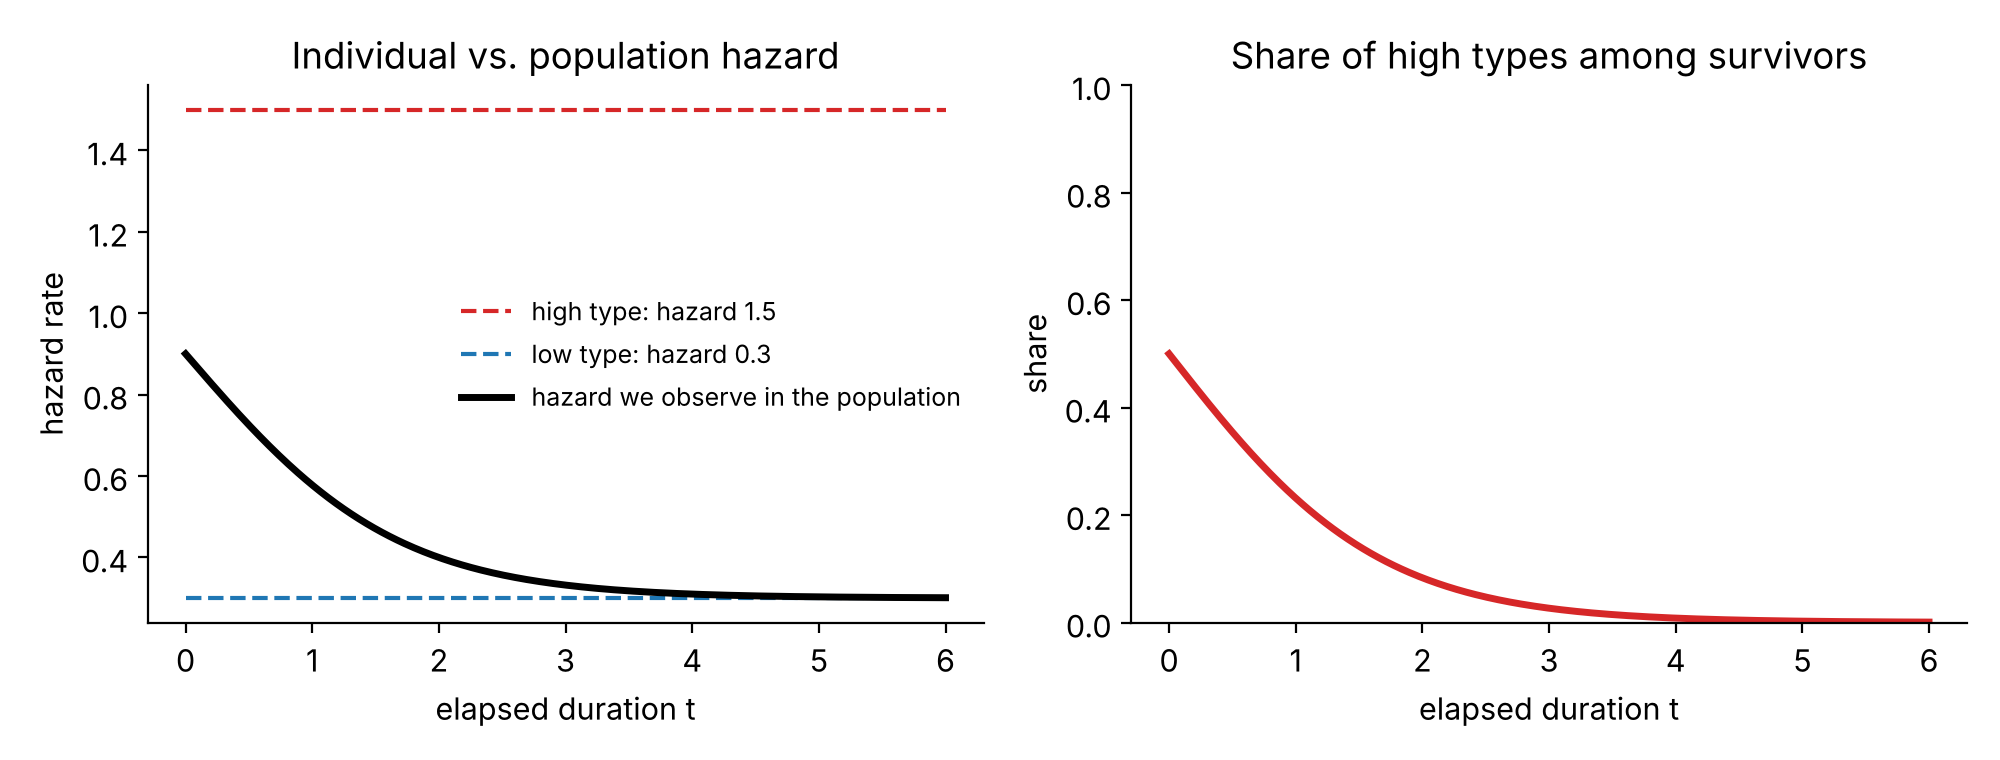
\includegraphics[width=\linewidth]{fig1_dynamic_selection.png}
    \end{column}
  \end{columns}

  \medskip
  \textbf{Trap or sorting?} A falling exit rate can be true duration dependence ($\lambda\downarrow$) or composition ($\E[V\mid T\ge t]\downarrow$). This is Heckman's \emph{true vs.\ spurious state dependence}, in continuous time.
\note{
\textbf{Derivation of the observed hazard.} The survival function is $\Pr(T>t)=\E[e^{-V\Lambda(t)}]$, with $\Lambda(t)=\int_0^t \lambda$. The population hazard is $-\frac{d}{dt}\log\Pr(T>t)=\lambda(t)\,\E[Ve^{-V\Lambda(t)}]/\E[e^{-V\Lambda(t)}]$. The ratio is the mean of $V$ under weights $e^{-V\Lambda(t)}$, i.e.\ $\E[V\mid T\ge t]$. The weight $e^{-V\Lambda(t)}$ is the probability that a type-$V$ person is still there. That is the whole idea of dynamic selection.

\textbf{Why it matters for treatment effects.} The people still unemployed and untreated at month 6 are a selected group. Comparing ``treated at month 6'' with ``not yet treated at month 6'' is only valid if we know how both groups were selected up to month 6. Every identification step below is about learning that selection.

\textbf{Figure.} Two types with \emph{constant} hazards 0.3 and 1.5 produce a population hazard that falls from 0.9 to 0.3. Nobody's hazard changes; only the composition does.

\textbf{The coin-flip view} matters later. Conditional on the hazard, the moment of the event is pure chance. This is the source of the ``randomization'' the paper exploits (footnote 15).
}
\end{frame}

% =====================================================================
\begin{frame}{Primer 2: the MPH model and the Laplace-transform toolkit}
  \textbf{Mixed proportional hazard:} $\theta(t\mid x,V)=\lambda(t)\,\varphi(x)\,V$, \quad $V\sim G$, \ $V\perp x$. Then
  \[ \Pr(T>t\mid x)=\E\big[e^{-V\varphi(x)\Lambda(t)}\big]=\Lap\big(\varphi(x)\Lambda(t)\big),\qquad \Lap(a):=\E[e^{-aV}]. \]
  \textbf{Toolkit.} $e^{-aV}$ is the probability that type $V$ survives to index $a$. So derivatives of $\log\Lap$ are \emph{moments among survivors}. In two dimensions, $\Lap(a,b)=\E[e^{-aV_Y-bV_S}]$:
  \[
    -\partial_a\log\Lap=\E[V_Y\mid\text{surv.}],\qquad
    -\partial_b\log\Lap=\E[V_S\mid\text{surv.}],\qquad
    \partial^2_{ab}\log\Lap=\cov(V_Y,V_S\mid\text{surv.}).
  \]
  \textbf{Single-risk identification (Elbers \& Ridder 1982), in 3 steps}
  \begin{enumerate}
    \item $t\downarrow0$: nobody has been selected out yet, so hazard ratios across $x$ give $\varphi(x)$ (needs $\E V<\infty$).
    \item At $t^*$ with $\Lambda(t^*)=1$: $\Pr(T>t^*\mid x)=\Lap(\varphi(x))$. Varying $x$ traces $\Lap$, hence $G$.
    \item Any $t$: solve $\Pr(T>t\mid x)=\Lap(\varphi(x)\Lambda(t))$ for $\Lambda(t)$.
  \end{enumerate}
  \textbf{We will run exactly this logic in two dimensions.}
\note{
\textbf{Where the toolkit comes from.} $\log\Lap(a,b)$ is the cumulant generating function of $(-V_Y,-V_S)$, evaluated under tilting by $e^{-aV_Y-bV_S}$. First derivative: $\partial_a\log\Lap=-\E[V_Ye^{-aV_Y-bV_S}]/\Lap=-\E_w[V_Y]$. Differentiate again in $b$: $\partial_b(-\E_w[V_Y])=\E_w[V_YV_S]-\E_w[V_Y]\E_w[V_S]=\cov_w(V_Y,V_S)$. The weights $w$ are survival probabilities, so ``$\E_w$'' means ``among survivors''. Two consequences we use repeatedly:
(i) the observed hazard is $\lambda\varphi\times(-\partial_a\log\Lap)$;
(ii) the dependence between $V_Y$ and $V_S$ among survivors (the selection) is a cross-derivative.

\textbf{Step 1 in detail.} The hazard is $\lambda(t)\varphi(x)\E[V\mid T\ge t,x]$. As $t\downarrow0$, $\E[V\mid T\ge t,x]\to\E[V]$, which is finite by assumption and the same for all $x$ because $V\perp x$. The ratio across $x$ and $x^*$ therefore tends to $\varphi(x)/\varphi(x^*)=\varphi(x)$. Note that identification uses the behaviour of short durations, where data are thin (critique on slide 17).

\textbf{Step 2.} The normalization $\Lambda(t^*)=1$ fixes the scale. Once $\varphi$ is known, $x\mapsto\Pr(T>t^*\mid x)$ is $\Lap$ evaluated at known points. Varying $x$ traces $\Lap$ on an interval. Laplace transforms are analytic, so $\Lap$ is then pinned down everywhere, and it determines $G$ uniquely.

\textbf{Step 3.} $\Lap$ is strictly decreasing, so invert.
}
\end{frame}

% =====================================================================
\begin{frame}{Set-up: potential outcomes indexed by treatment time}
  \begin{itemize}
    \item Treatments are dates $s\in[0,\infty]$ ($s=\infty$: never). Potential outcomes $Y^*(s)$; observed $Y=Y^*(S)$.
    \item \textbf{No anticipation:} $\theta_{Y^*(s)}(t)=\theta_{Y^*(s')}(t)$ for $t\le\min(s,s')$. A future treatment date does not affect today's hazard.\\
      Reacting to the sanction \emph{regime} is allowed (it is in every $Y^*(s)$), so the effect is \emph{``treated at $s$ vs.\ later, under this regime''}.
  \end{itemize}
  \begin{center}
  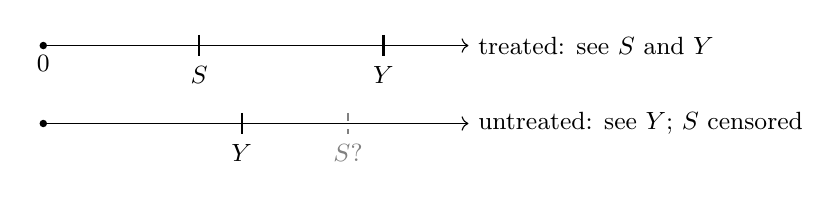
\begin{tikzpicture}[scale=0.9]
    \draw[->] (0,0) -- (6,0) node[right] {\small treated: see $S$ and $Y$};
    \fill (0,0) circle (1.5pt) node[below] {\small 0};
    \draw[thick] (2.2,0.15) -- (2.2,-0.15) node[below] {\small $S$};
    \draw[thick] (4.8,0.15) -- (4.8,-0.15) node[below] {\small $Y$};
    \draw[->] (0,-1.1) -- (6,-1.1) node[right] {\small untreated: see $Y$; $S$ censored};
    \fill (0,-1.1) circle (1.5pt);
    \draw[thick] (2.8,-0.95) -- (2.8,-1.25) node[below] {\small $Y$};
    \draw[dashed,gray] (4.3,-0.95) -- (4.3,-1.25) node[below] {\small $S$?};
  \end{tikzpicture}
  \end{center}
  \textbf{What the data reveal} (all conditional on $x$):
  \begin{itemize}
    \item $P_0(t)=\Pr(Y>t,S>t)$: nothing has happened by $t$;
    \item $h_Y(t)$, $h_S(t)$: rate of exiting untreated / of being treated, among those with nothing yet;
    \item $P_1(y\mid s)=\Pr(Y>y\mid S=s,\,Y>s)$: post-treatment survival of the \textbf{cohort treated at $s$}.
  \end{itemize}
  \textbf{Fact (Prop.~1):} any such data can be rationalized with no anticipation \emph{and} random assignment. So no anticipation is untestable, and we need a model of selection.
\note{
\textbf{Why index potential outcomes by a date.} A dynamically assigned binary treatment is really a continuum of mutually exclusive treatments, ``treated at $s$''. This is exactly the staggered-adoption set-up, where potential outcomes are indexed by the adoption cohort $g$ (slide 18).

\textbf{No anticipation.} The paper states it for integrated hazards; hazard paths agreeing up to $\min(s,s')$ is the same thing. In biostatistics this is a mild consistency condition. In economics it is behavioural: if a worker knows the sanction date and searches harder beforehand, it fails. If information arrives before treatment, the paper suggests treating the \emph{information shock} as the treatment.

\textbf{The data objects.} These four objects are equivalent to the paper's $(Q_S,Q_Y)$; see the appendix. The pre-treatment objects ($P_0,h_Y,h_S$) are classic \emph{competing-risks} data: two things can happen and we see which happens first. $P_1$ is the only place where the treatment effect can appear.

\textbf{Proposition 1 (de-emphasized).} By the Tsiatis/Miller result, any competing-risks data are generated by some \emph{independent} pair of latent durations. Use that pair for the pre-treatment part, and define the post-treatment hazard to match $P_1$. The result is a model with random assignment and no anticipation that fits the data perfectly. Two lessons: selection cannot be told from causality without structure, and anticipation cannot be detected. The paper's job-search illustration is in the appendix.
}
\end{frame}

% =====================================================================
\begin{frame}{The model}
  \textbf{Assumption 2 (selection on $(x,V)$):} $Y^*(\cdot)\perp S \mid (x,V)$, with $V$ time-invariant.

  \medskip
  \textbf{Model 1a.}
  \[
  \theta_Y(t\mid s,x,V)=\lambda_Y(t)\,\varphi_Y(x)\,V_Y\cdot\delta(t\mid s,x)^{\1\{t>s\}},\qquad
  \theta_S(t\mid x,V)=\lambda_S(t)\,\varphi_S(x)\,V_S,
  \]
  with $(V_Y,V_S)\sim G$ \textbf{arbitrarily dependent}, independent of $x$.

  \medskip
  \begin{itemize}
    \item Two MPH hazards. Their link through $\cov(V_Y,V_S)$ is the \textbf{selection on unobservables}.
    \item $\delta$ is the \textbf{causal effect}: a hazard multiplier after treatment. It may vary with $t$, $s$ (hence with $t-s$) and $x$, but not with $V$.
    \item No anticipation is built in: $\delta$ only acts for $t>s$.
    \item The same $x$ enters both hazards, so there is \textbf{no exclusion restriction}. $\lambda$'s, $\varphi$'s, $G$, $\delta$ are all nonparametric.
  \end{itemize}

  \medskip
  \textbf{Assn.~3:} $\{(\varphi_Y(x),\varphi_S(x))\}$ contains an open set of $\R^2$. \quad \textbf{Assn.~4:} $\E V_Y,\E V_S<\infty$.\\
  Normalizations: $\varphi(x^*)=1$, $\Lambda(t^*)=1$.
\note{
\textbf{How the model emerges from the set-up.} No anticipation says pre-treatment hazards do not depend on $s$. Assumption 2 says all dependence between $Y$ and $S$ runs through $(x,V)$. Together they imply: conditional on $(x,V)$, $Y$ and $S$ are linked \emph{only} through the causal factor $\delta$. That is why $\delta$ can be called a treatment effect.

\textbf{Why hazard-based assignment matters.} $S$ is modelled by a hazard, not by a threshold-crossing rule. So even conditional on $(x,V)$, $S$ is random: $\varphi_S(x)V_S\Lambda_S(S)$ is a unit exponential independent of $(x,V)$. This random component moves $S$ around without affecting $Y$ except through treatment. It is the analogue of an instrument (slide 8).

\textbf{Assumption 3 is not an exclusion restriction, but it is not free.} The covariates must move the two hazards \emph{non-proportionally}. With $\varphi_j(x)=e^{x'\beta_j}$ you need at least two continuous covariates and $(\beta_Y\ \beta_S)$ of full rank.

\textbf{Allowed but not shown:} mass points of $V$ at zero (never treated / never exit). Also $\Pr(Y=S)=0$ (continuous time, no ties).
}
\end{frame}

% =====================================================================
\begin{frame}{The selection problem at the moment of treatment}
  Fix a duration $s$. Write $a_s=\varphi_Y(x)\Lambda_Y(s)$, $b_s=\varphi_S(x)\Lambda_S(s)$.

  \medskip
  \textbf{Who is still at risk} (nothing happened by $s$):\quad $dG_{R_s}(v)\propto e^{-a_s v_Y-b_s v_S}\,dG(v)$.\\[2pt]
  \textbf{Who is treated at $s$:} the risk set, reweighted by the treatment intensity, \quad $dG_{s}(v)\propto v_S\,dG_{R_s}(v)$.

  \medskip
  \textbf{Exit hazards right at $s$:}
  \[
  \underbrace{\lambda_Y(s)\varphi_Y(x)\,\E_{R_s}[V_Y]}_{\text{not yet treated}}
  \qquad\text{vs.}\qquad
  \underbrace{\lambda_Y(s)\varphi_Y(x)\,\delta(s\mid s,x)\,\E_{s}[V_Y]}_{\text{just treated}}
  \]
  \[
  \frac{\text{just treated}}{\text{not yet treated}}
  \;=\;\delta(s\mid s,x)\times\underbrace{\Big(1+\frac{\cov_{R_s}(V_Y,V_S)}{\E_{R_s}[V_Y]\,\E_{R_s}[V_S]}\Big)}_{\text{selection factor}}
  \]
  \begin{itemize}
    \item If $V_Y\perp V_S$ among survivors, timing is as good as random at $s$: the ratio \emph{is} the causal effect.
    \item Otherwise we need the \textbf{joint distribution of types among survivors}. The pre-treatment data will supply it.
  \end{itemize}
\note{
\textbf{This slide is the heart of the paper's logic.} It reduces the selection problem to one object.

\textbf{Derivation.} Being at risk at $s$ means $Y>s$ and $S>s$. Given $V$, no anticipation means $Y$'s hazard before $s$ is the untreated one, so the probability of being at risk is $e^{-a_sV_Y}e^{-b_sV_S}$ (Assumption 2 lets the two terms multiply). By Bayes' rule, the type distribution in the risk set is $G$ reweighted by that probability. Among those at risk, the chance of being treated in $[s,s+ds)$ is $\lambda_S(s)\varphi_S(x)V_S\,ds$. So the treated cohort is the risk set reweighted by $V_S$.

The mean of $V_Y$ in the treated cohort is
$\E_s[V_Y]=\E_{R_s}[V_YV_S]/\E_{R_s}[V_S]=\E_{R_s}[V_Y]+\cov_{R_s}(V_Y,V_S)/\E_{R_s}[V_S]$.
Divide by $\E_{R_s}[V_Y]$ to get the selection factor.

\textbf{Reading it.} Suppose low-motivation people (low $V_Y$) are sanctioned more (high $V_S$), so the covariance is negative. Then the just-treated have low $V_Y$, and the naive comparison \emph{understates} a positive effect of sanctions on exit. This is the classic ``Heckman selection'' structure, with a control-function-like correction factor.

\textbf{The ratio on the left is data.} The hazard of the just-treated is $-\partial_y\log P_1(y\mid s)$ as $y\downarrow s$; the hazard of the not-yet-treated is $h_Y(s)$. So everything hinges on the selection factor, a feature of the joint distribution of $(V_Y,V_S)$ among those at risk at $s$.
}
\end{frame}

% =====================================================================
\begin{frame}{Timing as an instrument}
  \footnotesize
  \begin{tabular}{p{0.2\textwidth}p{0.29\textwidth}p{0.41\textwidth}}
    \toprule
    & Static selection / IV & Timing of events \\
    \midrule
    Exogenous variation in treatment
    & excluded variable $Z$
    & the timing shock: given $(x,V)$, $S=\Lambda_S^{-1}\!\big(\tfrac{E_S}{\varphi_S(x)V_S}\big)$, $E_S\sim\text{Exp}(1)$ \\[3pt]
    What is excluded from the outcome
    & the \emph{variable} $Z$
    & the \emph{shock} $E_S$ (via Assn.~2) \\[3pt]
    Correcting for who selects in
    & control function $\E[U\mid D=1,Z]$
    & selection factor / $G_s$, from the competing-risks data \\[3pt]
    Covariate requirement
    & $Z$ shifts $D$, not $Y$
    & $x$ shifts both hazards, \emph{non-proportionally} (Assn.~3) \\
    \bottomrule
  \end{tabular}

  \normalsize
  \bigskip
  \textbf{Why timing is informative.} The treatment acts only \emph{after} $S$; $V$ acts \emph{throughout}.
  \begin{itemize}
    \item Causal effect $\Rightarrow$ \textbf{local} dependence: exits bunch right after $S$, \emph{whenever} $S$ occurs.
    \item Selection $\Rightarrow$ \textbf{global} dependence: early-treated people are early leavers in general.
  \end{itemize}
  In a static latent-index model the treatment effect needs an exclusion restriction. Here the timing replaces it.
\note{
\textbf{The point of the table.} An IV design needs two things: (i) variation in treatment that is unrelated to the outcome's unobservables, and (ii) a way to handle the fact that the people who take treatment are selected.

(i) In a static threshold model $D=\1\{\mu(Z)>U\}$, treatment is deterministic given $(Z,U)$, so exogenous variation must come from an excluded $Z$. With hazard-based assignment, treatment \emph{timing} is still random given $(x,V)$. The representation uses the fact that $\varphi_S(x)V_S\Lambda_S(S)$ is unit exponential. The exclusion restriction has not disappeared: it moved from an observed variable to an unobserved shock. Assumption 2 says the timing shock $E_S$ is independent of everything that drives $Y$. Be candid about this in the talk.

(ii) The selection correction is the analogue of a control function. Here it is not estimated from an excluded instrument; it comes from the competing-risks part of the data (next three slides).

\textbf{Local vs.\ global.} This is the paper's own intuition (Section 3.2) and the basis of the companion paper on testing the sign of $\delta$. The figure on the next slide makes it concrete.
}
\end{frame}

% =====================================================================
\begin{frame}{What the data look like}
  \centering
  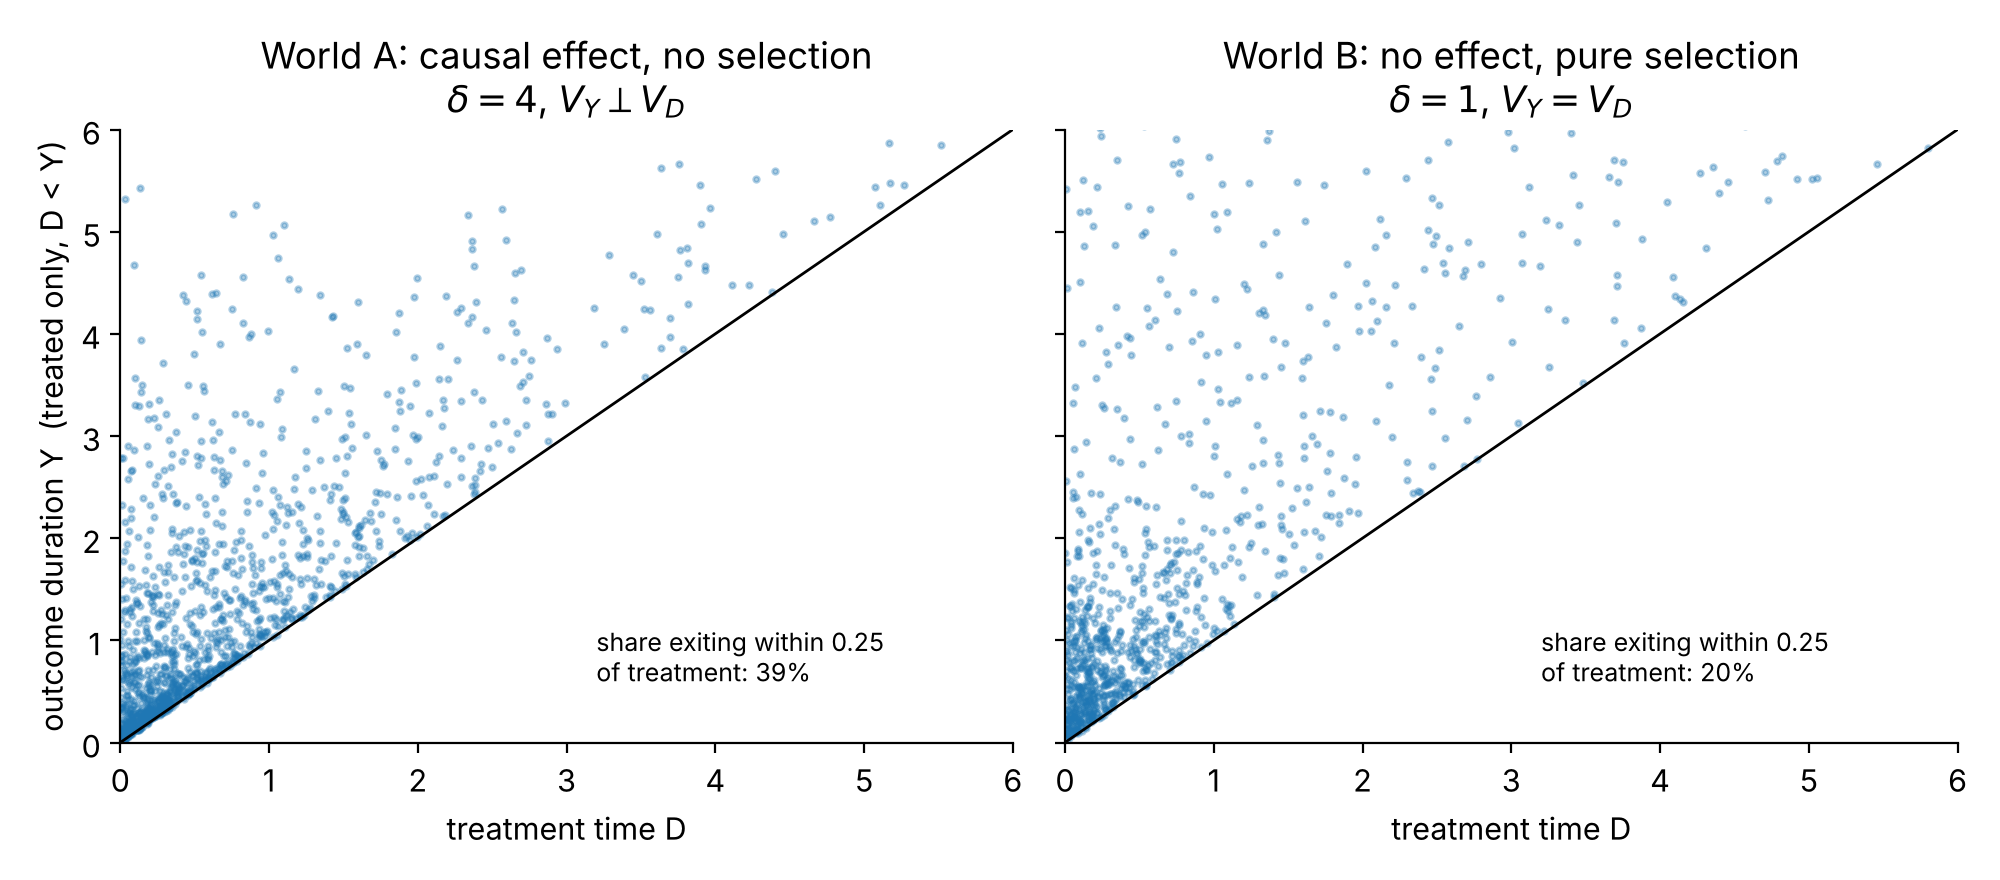
\includegraphics[width=0.85\linewidth]{fig3_local_vs_global.png}

  \raggedright\small
  Treated observations only. Left: $\delta=4$, independent frailties. Right: $\delta=1$, $V_Y=V_S$. A causal effect makes points hug the diagonal \emph{at every $S$}. Selection produces quick exits only where high types are concentrated (small $S$).
\note{
\textbf{Simulation.} Two types (0.25 and 2), constant baseline hazards. World A: types for $Y$ and $S$ drawn independently, and treatment multiplies the exit hazard by 4. World B: one common type, no effect.

Both worlds show a positive association between $S$ and $Y$, and in both some people exit quickly after treatment. The difference is \emph{where} the quick exits are. In A they occur after treatment at any $S$; in B they are concentrated at small $S$, where the high types still are. The formal argument quantifies exactly this: how many quick post-treatment exits would we expect from selection alone, given the types at risk at $s$?

Script: \texttt{figures/make\_figures.py}.
}
\end{frame}

% =====================================================================
\begin{frame}{The pre-treatment data are a competing-risks problem}
  Before treatment there are two latent clocks: $Y^0$ (exit if never treated) and $S$. Their joint survival is
  \[ \Pr(Y^0>y,\,S>s\mid x)=\Lap\big(\varphi_Y(x)\Lambda_Y(y),\;\varphi_S(x)\Lambda_S(s)\big). \qquad \text{($\delta$ does not appear!)}\]
  We only see the \emph{first} event: the diagonal $y=s=t$, i.e.\ $P_0(t\mid x)=\Lap(a_t(x),b_t(x))$, plus which event it was.

  \smallskip
  \textbf{Tsiatis (1975):} without structure, any such data are generated by \emph{independent} clocks. The dependence, i.e.\ the selection, is unidentified.

  \begin{center}
    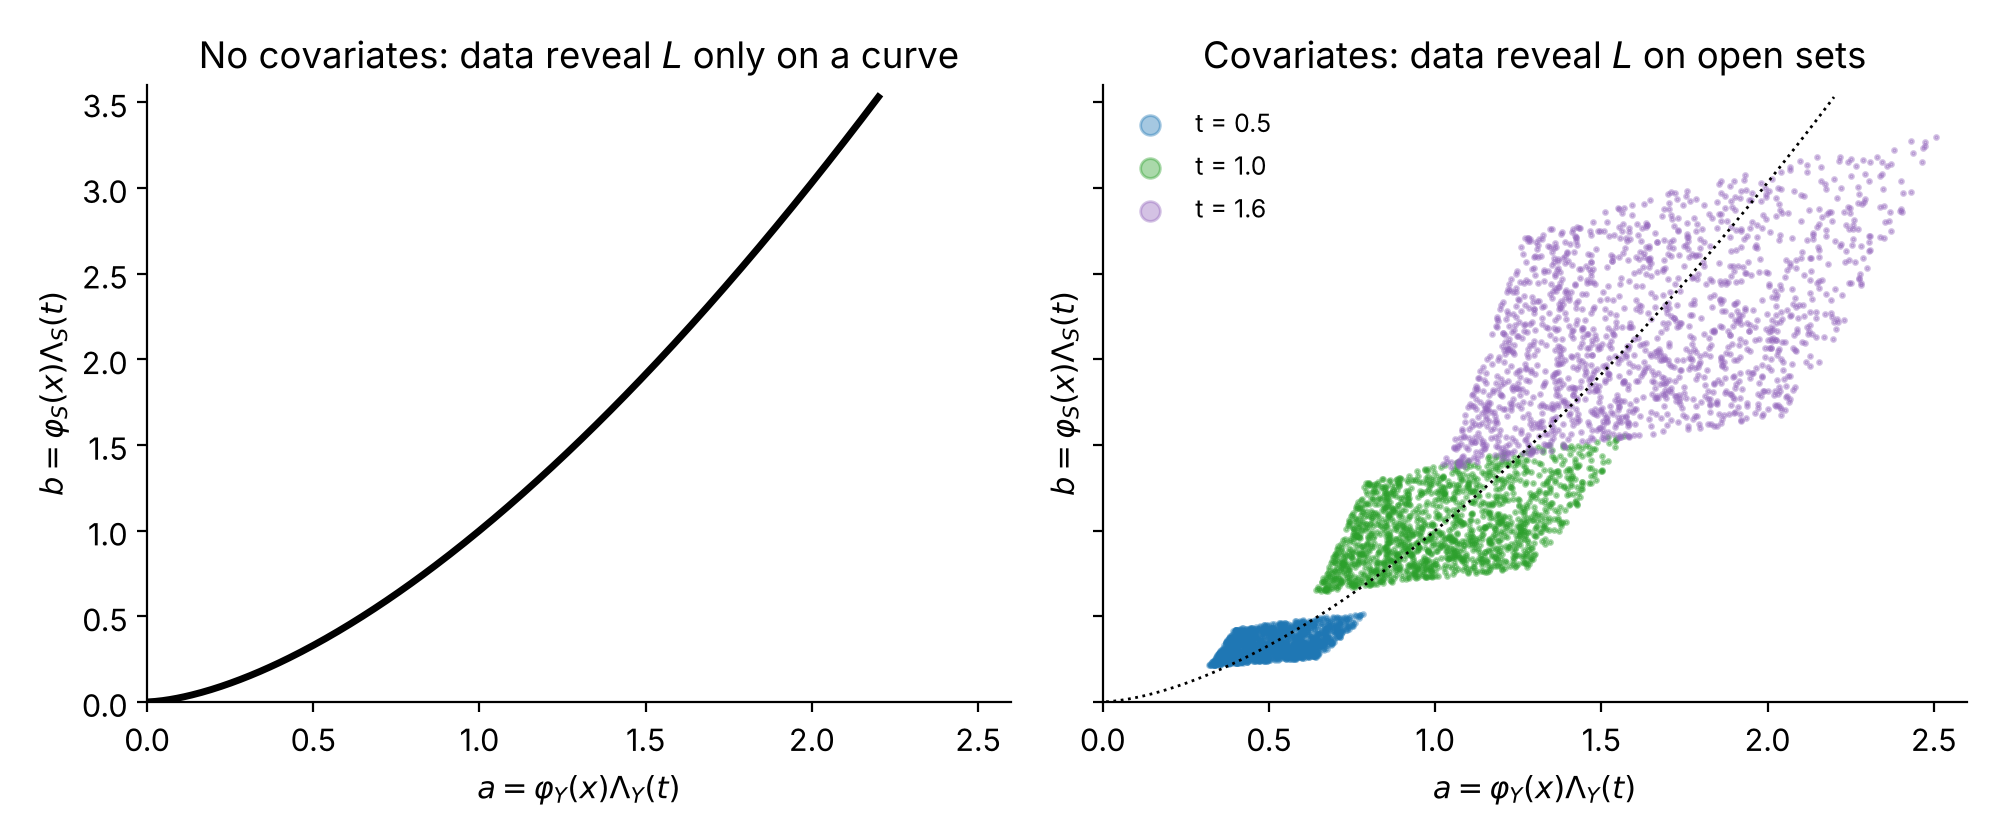
\includegraphics[width=0.56\linewidth]{fig4_competing_risks_geometry.png}
  \end{center}
  \vspace{-6pt}
  \small Without $x$, the data reveal $\Lap$ only along a curve $t\mapsto(\Lambda_Y(t),\Lambda_S(t))$. A curve cannot pin down a function of two variables. With $x$ shifting the two hazards separately, the data reveal $\Lap$ on \emph{open sets}.
\note{
\textbf{Why this is the crucial step.} Slide 7 showed that everything hinges on the joint distribution of $(V_Y,V_S)$. The only place to learn it without using the outcome we want to explain is the pre-treatment period. There, by no anticipation, nothing causal is going on. We just watch two clocks race.

\textbf{The joint survival.} Given $V$, the two clocks are independent with integrated hazards $\varphi_Y\Lambda_YV_Y$ and $\varphi_S\Lambda_SV_S$. Integrating over $G$ gives the bivariate Laplace transform evaluated at the two indices.

\textbf{Geometry of non-identification.} With no covariates, data at duration $t$ tell us $\Lap$ at one point $(\Lambda_Y(t),\Lambda_S(t))$. As $t$ varies we learn $\Lap$ along a curve, plus the slopes of $\Lap$ in the two directions along that curve (from the cause-specific hazards). Many bivariate distributions agree on those values, including independent ones. That is Tsiatis' result.

\textbf{How covariates break it.} At a fixed $t$, varying $x$ moves the point to $(\varphi_Y(x)\Lambda_Y(t),\varphi_S(x)\Lambda_S(t))$. If the two $\varphi$'s move independently (Assumption 3), the point sweeps out a two-dimensional patch. Knowing an analytic function on any open patch determines it everywhere. This is why Assumption 3 must be two-dimensional, and it is what makes the selection identified.
}
\end{frame}

% =====================================================================
\begin{frame}{Identifying the competing-risks part (Prop.~2): three steps}
  \textbf{Step 1: $\varphi$'s from short durations} (nobody has been selected out yet):
  \[ \frac{h_Y(t\mid x)}{h_Y(t\mid x^*)}=\frac{\varphi_Y(x)\,\E[V_Y\mid R_t,x]}{\E[V_Y\mid R_t,x^*]}\;\xrightarrow{\;t\downarrow0\;}\;\varphi_Y(x),\qquad\text{same for }\varphi_S. \]
  Uses \emph{which} event happened and $\E V<\infty$.

  \medskip
  \textbf{Step 2: $G$ at the normalization date} ($\Lambda_Y(t^*)=\Lambda_S(t^*)=1$):
  \[ P_0(t^*\mid x)=\Lap\big(\varphi_Y(x),\varphi_S(x)\big). \]
  Known points fill an open set (Assn.~3), so $\Lap$ is known there. $\Lap$ is real-analytic, so it is known on $(0,\infty)^2$, and $\Lap$ determines $G$, \textbf{including the dependence between $V_Y$ and $V_S$}.

  \medskip
  \textbf{Step 3: baselines.} For every $t$, $(\Lambda_Y(t),\Lambda_S(t))$ is the unique $(a,b)$ with
  \[ P_0(t\mid x)=\Lap\big(\varphi_Y(x)\,a,\;\varphi_S(x)\,b\big)\quad\text{for all }x. \]

  \medskip
  $\Rightarrow$ $\lambda_Y,\lambda_S,\varphi_Y,\varphi_S,G$ are identified \textbf{without touching post-treatment data}.
\note{
\textbf{Relation to the paper.} The paper proves Proposition 2 by citing Abbring \& Van den Berg (2003, JRSSB). The three steps here are a self-contained route that makes the logic visible. It is Elbers--Ridder (slide 4) in two dimensions.

\textbf{Step 1.} The cause-specific hazard of exiting untreated among those at risk is $h_Y(t\mid x)=\lambda_Y(t)\varphi_Y(x)\E[V_Y\mid R_t,x]=\lambda_Y(t)\varphi_Y(x)\big(-\partial_a\log\Lap\big)(a_t,b_t)$. As $t\downarrow0$ the risk set is the whole population. Because $V\perp x$ and $\E V_Y<\infty$, the conditional mean tends to the same constant for all $x$, and $\lambda_Y(t)$ cancels in the ratio.

\textbf{Step 2.} Only the probability of ``no event yet'' is needed here; the cause-specific information was used in step 1. Analyticity: $\Lap(a,b)=\E e^{-aV_Y-bV_S}$ is real-analytic on $(0,\infty)^2$, and two analytic functions that agree on an open set agree on the whole connected domain. A distribution on $[0,\infty)^2$ is determined by its Laplace transform.

\textbf{Step 3.} Uniqueness is proved in the appendix. Idea: if two pairs fit, then $\Lap(u,v)=\Lap(ku,mv)$ for some $(k,m)\neq(1,1)$. Iterating forces $\Lap$ to be constant, which contradicts it being strictly decreasing.

\textbf{What is used where.} No anticipation: the pre-treatment hazard of $Y$ is the untreated one, so $\delta$ is absent. Assumption 2: the clocks are independent given $V$. MPH: the index structure. Assumption 4: step 1. Assumption 3: step 2.
}
\end{frame}

% =====================================================================
\begin{frame}{Where the selection shows up in the data}
  From the toolkit, applied to the observed $P_0(t\mid x)=\Lap(a_t(x),b_t(x))$:
  \[ \frac{\partial^2\log P_0}{\partial a\,\partial b}=\cov\big(V_Y,V_S\mid \text{nothing happened by }t,\,x\big). \]
  \begin{itemize}
    \item $V_Y\perp V_S$ $\iff$ $\Lap(a,b)=\Lap_Y(a)\Lap_S(b)$ $\iff$ $\log P_0$ is \textbf{additively separable} in the two covariate indices.
    \item Selection on unobservables $=$ an \textbf{interaction}: a covariate that raises the treatment hazard changes how the exit index affects survival.
    \item Seeing an interaction requires the two indices to move separately (Assn.~3). That is where the instrument-like requirement hides: \emph{no exclusion, but non-proportional covariate effects}.
  \end{itemize}

  \medskip
  The selection factor of slide 7 is then a function of identified objects:
  \[ 1+\frac{\cov_{R_s}(V_Y,V_S)}{\E_{R_s}V_Y\;\E_{R_s}V_S}=\frac{\Lap\,\Lap_{ab}}{\Lap_a\,\Lap_b}\Big|_{(a_s,b_s)}
  \quad\Rightarrow\quad
  \delta(s\mid s,x)=\frac{\text{observed hazard ratio at }s}{\Lap\Lap_{ab}/(\Lap_a\Lap_b)}. \]
\note{
\textbf{This answers ``how does competing risks identify the selection''.} The covariance of unobserved types among survivors is a cross-partial of the log probability that nothing has happened yet, taken with respect to the two covariate indices.

\textbf{Intuition.} Suppose $x_1$ mainly raises the treatment hazard and $x_2$ mainly raises the exit hazard. With independent types, their effects on $\log P_0$ add up. With correlated types, raising treatment intensity removes (through treatment) people whose exit propensity is also unusual. This changes the composition of who remains, and so changes the marginal effect of $x_2$ on survival. That interaction is the fingerprint of selection.

\textbf{Algebra for the selection factor.} $\E_{R_s}V_Y=-\Lap_a/\Lap$, $\E_{R_s}V_S=-\Lap_b/\Lap$, and $\E_{R_s}[V_YV_S]=\Lap_{ab}/\Lap$. Hence $\E_{R_s}[V_YV_S]/(\E V_Y\E V_S)=\Lap\Lap_{ab}/(\Lap_a\Lap_b)$, which equals $1+\cov/(\E\E)$. With independent types this is exactly 1.

\textbf{Caveat.} In practice, functional form ($\varphi=e^{x'\beta}$, parametric $\lambda$, discrete $G$) does much of the work that the open-set argument does in theory.
}
\end{frame}

% =====================================================================
\begin{frame}{Stripping out selection after treatment (Prop.~3)}
  For $y>s$, with $D(y\mid s,x)=\int_s^y\lambda_Y(\tau)\delta(\tau\mid s,x)\,d\tau$ the integrated post-treatment hazard,
  \[
  P_1(y\mid s,x)=\E_{G_s}\!\Big[e^{-\varphi_Y(x)V_Y\,D(y\mid s,x)}\Big]
  =\frac{\Lap_b\big(a_s+\varphi_Y(x)D(y\mid s,x),\;b_s\big)}{\Lap_b(a_s,b_s)}.
  \]
  \begin{itemize}
    \item The left side is data. On the right, everything except $D$ is known from Prop.~2.
    \item The right side is strictly decreasing in $D$, so \textbf{invert} to get $D(y\mid s,x)$. Then $\delta(y\mid s,x)=\partial_yD/\lambda_Y(y)$.
  \end{itemize}

  \medskip
  \textbf{Two selection problems, both solved by knowing $G$:}
  \begin{enumerate}
    \item \textbf{Selection into treatment at $s$:} the $V_S$-tilt of $G_s$ (absent if $V_Y\perp V_S$).
    \item \textbf{Selection out after $s$:} the treated cohort's survivors drift toward low $V_Y$. This happens whenever $V_Y$ varies, \emph{even with random timing}. So hazard ratios at longer horizons $\neq\delta$.
  \end{enumerate}
\note{
\textbf{Derivation (this is the paper's eq.~(10), normalized).} Given $V$, the density of being treated at $s$ while still unemployed is $\lambda_S(s)\varphi_S V_S\,e^{-b_sV_S}e^{-a_sV_Y}$. Survival from $s$ to $y$ after treatment is $e^{-\varphi_YV_YD(y\mid s)}$. Multiply, integrate over $G$, and divide by the same expression with $y=s$:
$P_1=\E[V_Se^{-(a_s+\varphi_YD)V_Y-b_sV_S}]/\E[V_Se^{-a_sV_Y-b_sV_S}]$.
Since $\Lap_b=-\E[V_Se^{-aV_Y-bV_S}]$, this is the displayed ratio. The paper's (10) is the numerator: $\partial Q_S(y,s)/\partial s=\varphi_S\lambda_S(s)\Lap_b(\ldots)$.

\textbf{Monotonicity.} $\partial_a\Lap_b=\E[V_YV_Se^{\cdots}]>0$, so $\Lap_b$ (which is negative) increases toward 0 as $D$ grows. The ratio therefore falls strictly with $D$.

\textbf{Point 2 is where the duration setting departs from standard treatment-effect intuition.} Suppose timing is random ($V_Y\perp V_S$). The treated cohort starts with the same types as the controls, but if $\delta>1$ its high-$V_Y$ members leave faster. After a while the surviving treated are a more negatively selected group than the surviving controls. A naive hazard ratio at horizon $y-s$ then underestimates $\delta$. Epidemiology knows this as ``the hazards of hazard ratios'' (Hern\'an 2010). The model handles it because $G$ is known.

\textbf{Slide 7 is the special case $y\downarrow s$} of this slide.
}
\end{frame}

% =====================================================================
\begin{frame}{The identification chain, and where each assumption is used}
  \centering
  \resizebox{\linewidth}{!}{%
  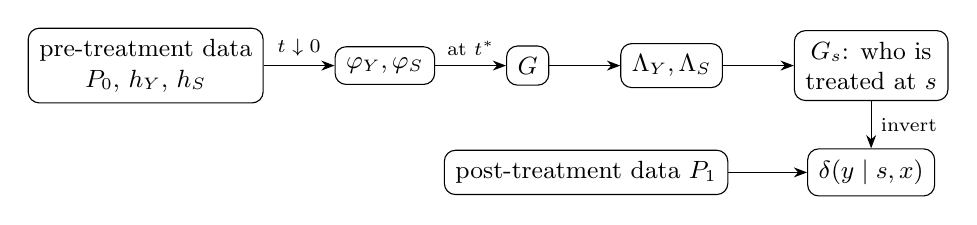
\begin{tikzpicture}[node distance=0.6cm and 0.9cm, box/.style={draw,rounded corners,align=center,font=\small,inner sep=4pt}, >=Stealth]
    \node[box] (pre) {pre-treatment data\\$P_0,\,h_Y,\,h_S$};
    \node[box,right=of pre] (phi) {$\varphi_Y,\varphi_S$};
    \node[box,right=of phi] (G) {$G$};
    \node[box,right=of G] (Lam) {$\Lambda_Y,\Lambda_S$};
    \node[box,right=of Lam] (Gs) {$G_s$: who is\\treated at $s$};
    \node[box,below=of Gs] (delta) {$\delta(y\mid s,x)$};
    \node[box,left=1.0cm of delta] (post) {post-treatment data $P_1$};
    \draw[->] (pre) -- node[above,font=\scriptsize]{$t\downarrow0$} (phi);
    \draw[->] (phi) -- node[above,font=\scriptsize]{at $t^*$} (G);
    \draw[->] (G) -- (Lam);
    \draw[->] (Lam) -- (Gs);
    \draw[->] (Gs) -- node[right,font=\scriptsize]{invert} (delta);
    \draw[->] (post) -- (delta);
  \end{tikzpicture}}

  \raggedright
  \medskip
  \small
  \begin{tabular}{p{0.27\textwidth}p{0.6\textwidth}}
    \toprule
    Assumption & Role \\
    \midrule
    No anticipation & pre-treatment period is a clean competing-risks problem ($\delta$ absent) \\
    Selection only via $(x,V)$ & clocks independent given $V$; treated $=$ risk set reweighted by $V_S$ \\
    MPH separability, $V\perp x$ & index structure $\Lap(\varphi\Lambda)$ behind all three steps \\
    $\E V<\infty$ & step 1 (short-duration hazard ratios) \\
    2-D covariate variation & step 2: trace $\Lap$ on an open set $\Rightarrow$ identifies the dependence \\
    \bottomrule
  \end{tabular}
\note{
\textbf{Use this slide to recap.} If the audience retains one picture, it should be this chain.

Information flows from the pre-treatment data, where nothing causal happens, to the structure of selection. The post-treatment data are then used only once, at the end, to read off $\delta$ after the selection has been removed.

\textbf{What is \emph{not} on the list:} an excluded instrument, selection on observables, parametric functional forms, or multiple spells.
}
\end{frame}

% =====================================================================
\begin{frame}{Heterogeneous effects (Model 1b, Prop.~4)}
  \[
  \theta_Y(t\mid s,x,V)=\begin{cases}\lambda_Y(t)\varphi_Y(x)V_Y & t\le s\\ \lambda_\Delta(t)\varphi_\Delta(x)V_\Delta & t>s\end{cases},
  \qquad (V_Y,V_\Delta,V_S)\sim G_\Delta,
  \]
  \[
  \text{so the effect is}\quad
  \delta(t\mid x,V)=\frac{\lambda_\Delta(t)\varphi_\Delta(x)V_\Delta}{\lambda_Y(t)\varphi_Y(x)V_Y}.
  \]
  \begin{itemize}
    \item \textbf{Gained:} the effect varies with unobservables, and $V_\Delta$ may correlate with $V_S$. This allows \textbf{selection on gains} (Roy-type sorting).
    \item \textbf{Lost:} $\delta$ can no longer depend on the treatment date $s$.
    \item \textbf{Why it works:} after $S$, the residual duration of the treated cohort is again MPH, in $\Lambda_\Delta(y)-\Lambda_\Delta(s)$ with frailty $V_\Delta$, so Elbers--Ridder can be rerun on it.
    \item \textbf{Extra assumptions:} variation in $\varphi_\Delta(x)$, and $\E[V_\Delta V_S]<\infty$. The moment is of the \emph{product} because the treated cohort is tilted by $V_S$.
  \end{itemize}
\note{
\textbf{Why the trade-off arises.} In Model 1a, $\delta(t\mid s,x)$ can be any function, but it is common to all types. Identification inverts $P_1$ for a single unknown function $D$ given a known $G_s$. In Model 1b the post-treatment hazard has its own frailty, so after treatment there is a new unknown distribution (that of $V_\Delta$ in the treated cohort). Identifying it requires running the MPH argument again on post-treatment durations. That argument needs the post-treatment hazard to be proportional and the same function for all $s$, so dependence on $s$ is ruled out.

\textbf{Proof idea (appendix).} Take second derivatives of the data with respect to $(y,s)$. Letting $y,s\downarrow0$ identifies $\varphi_\Delta$ (the analogue of step 1). Then the trivariate Laplace transform is traced on an open set (the analogue of step 2).
}
\end{frame}

% =====================================================================
\begin{frame}{Multiple spells: the within estimator (Model 2c, Prop.~6)}
  Strata (same person twice, siblings, \ldots) with two spells sharing the same unobservables:
  \[ \theta_{Y_k}(t\mid S_k,V)=\lambda_{Y_k}(t)\,V_Y(t)\,\delta_k(t\mid S_k)^{\1\{t>S_k\}},\qquad k=1,2,\quad \lambda_{Y_1}\equiv1. \]
  $V_Y(t)$ may be \textbf{any process common to both spells}, and there is \textbf{no model for $S_k$}.

  \medskip
  Given that the first exit in the stratum happens at $t$, which spell was it? $V_Y(t)$ \textbf{cancels}:
  \[ \Pr(\text{spell 1}\mid t,\text{histories},V)=\frac{\theta_{Y_1}(t)}{\theta_{Y_1}(t)+\theta_{Y_2}(t)}. \]
  \small
  \begin{tabular}{lll}
    \toprule
    treated at $t$ & $\Pr(\text{spell 1 first})$ & identifies \\
    \midrule
    neither & $1/(1+\lambda_{Y_2})$ & $\lambda_{Y_2}$ \\
    spell 1 only & $\delta_1/(\delta_1+\lambda_{Y_2})$ & $\delta_1$ \\
    spell 2 only & $1/(1+\lambda_{Y_2}\delta_2)$ & $\delta_2$ \\
    both & $\delta_1/(\delta_1+\lambda_{Y_2}\delta_2)$ & (overidentifying) \\
    \bottomrule
  \end{tabular}

  \normalsize
  \medskip
  \textbf{Cox partial likelihood $=$ conditional logit $=$ fixed effects.} \textbf{Cost:} $V$ identical across spells, and \textbf{no causal links across spells}.
\note{
\textbf{Why this is the panel analogue.} In linear panels the within transformation removes the individual effect. Here, conditioning on ``one of the two spells ends at $t$'' removes the stratum effect, because it multiplies both hazards. This is Cox's partial-likelihood logic, applied to strata (Holt \& Prentice 1974; Ridder \& Tunal\i{} 1999).

\textbf{What is gained relative to the single-spell case.} No covariates are needed, no finite means, no MPH assumption on how $V$ interacts with time ($V_Y(t)$ can be an arbitrary process), and no model for treatment assignment at all.

\textbf{What it costs.} The unobservable must be \emph{exactly} shared across the two spells. The first spell (or its treatment) must not causally affect the second. For repeated unemployment spells of the same person, that rules out scarring and learning across spells (see the traps discussion on slide 19).

\textbf{Models 2a/2b} (Prop.~5) are MPH versions that also identify $G$; see the appendix.
}
\end{frame}

% =====================================================================
\begin{frame}{What is traded, and critiques}
  \begin{columns}[T]
    \begin{column}{0.45\textwidth}
      \textbf{Not needed}
      \begin{itemize}
        \item an excluded instrument
        \item selection on observables
        \item parametric functional forms
        \item multiple spells (single-spell results)
      \end{itemize}
      \textbf{Needed}
      \begin{itemize}
        \item no anticipation (untestable)
        \item time-invariant unobservables, $V\perp x$
        \item MPH proportionality
        \item 2-D, non-proportional covariate variation
        \item finite means; continuous time
      \end{itemize}
    \end{column}
    \begin{column}{0.53\textwidth}
      \textbf{Critiques}
      \begin{itemize}
        \item Identification comes from $t\downarrow0$, where data are thin. In practice: parametric $\lambda$, discrete $G$ (Heckman--Singer); Monte Carlo evidence in Gaure, R\o ed \& Zhang (2007).
        \item Discrete time: sanction and exit in the same month blur the local signal.
        \item $\delta$ is a hazard ratio \emph{conditional on $V$}. Effects on mean duration or population survival require $G$.
        \item Transitory shocks hitting both hazards (the caseworker reacts to this week's low effort) violate Assn.~2.
      \end{itemize}
    \end{column}
  \end{columns}
\note{
\textbf{One-sentence summary of the trade.} The excluded \emph{variable} is replaced by (i) an excluded timing \emph{shock}, (ii) multiplicative separability, (iii) time-invariant heterogeneity, and (iv) no anticipation.

\textbf{On the last critique.} This is the most common objection in the sanctions literature. Sanctions are typically triggered by observed non-compliance, which may reflect a temporary drop in search effort that also lowers the exit rate. That is a time-varying unobservable affecting both hazards, which Model 1a excludes. Model 2c partly addresses it, but only with multiple spells.
}
\end{frame}

% =====================================================================
\begin{frame}{Connection: staggered adoption DiD}
  \textbf{Same skeleton}
  \begin{itemize}
    \item $Y^*(s)$ $\leftrightarrow$ $Y_t(g)$, potential outcomes indexed by adoption cohort.
    \item No anticipation is \emph{the same assumption} (Callaway \& Sant'Anna 2021; Sun \& Abraham 2021; Borusyak, Jaravel \& Spiess 2024).
    \item The risk set $R_s$ $\leftrightarrow$ the \emph{not-yet-treated} comparison group.
    \item $\delta(t\mid s)$ varies by cohort $s$ and event time $t-s$: the heterogeneity that breaks TWFE.
  \end{itemize}
  \textbf{Differences}
  \begin{itemize}
    \item Selection: \emph{parallel trends} (additive, in levels) vs.\ \emph{time-invariant frailty} (multiplicative, in hazards) plus a random timing shock.
    \item \textbf{Attrition from an absorbing exit:} the treatment changes who remains (slide 13), so ``parallel trends in hazards'' fails \emph{even under random timing}.\\
      DiD on survival probabilities $\to$ a population estimand; ToE $\to$ the individual hazard effect $\delta$, which needs $G$.
    \item If timing is random given observables (\emph{dynamic CIA}), treat later treatment as independent censoring. Population effects on survival are then identified nonparametrically (Fredriksson \& Johansson 2008; Crépon et al.\ 2009; Vikström 2017). ToE is the tool when timing is selected on \emph{unobservables}.
  \end{itemize}
\note{
\textbf{Why the analogy is exact on the skeleton.} Both literatures face a treatment that switches on at a unit-specific date and stays on. Both index potential outcomes by that date. Both impose no anticipation. The comparison ``treated at $s$ vs.\ not yet treated at $s$'' on slide 7 is the event-time-zero comparison of Callaway--Sant'Anna using not-yet-treated controls.

\textbf{Where they part.} In DiD every unit stays in the panel and the outcome is a level. In duration data the outcome is the exit itself, so the sample at risk changes as a \emph{result} of the outcome, and of the treatment. Even if treatment timing were randomly assigned, post-treatment hazard comparisons are contaminated by differential attrition. That is a dynamic-selection bias with no analogue in a balanced panel.

\textbf{Two estimands.} The population effect on survival curves can be obtained by design-based arguments under dynamic CIA. The individual-level hazard effect $\delta$ (needed for structural or behavioural interpretation, e.g.\ search theory) needs a model of $V$.

\textbf{Check citations before the talk.}
}
\end{frame}

% =====================================================================
\begin{frame}{Connection: sequential exogeneity, feedback, and traps}
  \textbf{Sequential exogeneity and feedback}
  \begin{itemize}
    \item A hazard is an intensity relative to the past: $dN_Y(t)-\theta_Y(t\mid\text{past},V)\,dt$ is a martingale difference. This is a continuous-time \emph{sequential moment condition}. No anticipation means treatment is \emph{predetermined}.
    \item In a single absorbing spell, outcome$\to$treatment feedback is degenerate (the only outcome history is ``still here''). The bite is on transitory shocks: $S$ may depend on permanent $V$, not on shocks to the exit rate. This is \emph{strict exogeneity given a fixed effect}.
    \item Model 2c moves toward sequential exogeneity: $S$ is unmodelled and may track a time-varying common $V_Y(t)$, at the cost of needing multiple spells.
  \end{itemize}
  \textbf{Traps: state dependence vs.\ permanent heterogeneity}
  \begin{itemize}
    \item The model separates three objects: $\lambda_Y\downarrow$ (true duration dependence: a trap), $G$ (permanent heterogeneity), and $\delta$ (the effect of an intervention).
    \item Traps suggest \emph{when} you intervene matters: $\delta(t\mid s)$ varying in $s$. Model 1a allows it; Model 1b rules it out.
    \item Multiple-spell results assume no cross-spell effects, i.e.\ they \emph{rule out} lagged duration dependence, the across-spell trap mechanism.
  \end{itemize}
\note{
\textbf{Sequential exogeneity.} In panel data, sequential exogeneity, $\E[u_t\mid x_t,x_{t-1},\ldots,\alpha]=0$, allows future regressors to respond to past outcome shocks (feedback). In counting-process language, the intensity is defined relative to a filtration, and the martingale property is the same type of sequential condition. Treatment history up to $t^-$ can be in the conditioning set, which is exactly no anticipation.

What ToE adds is the fixed effect $V$, together with the assumption that treatment does not respond to transitory shocks that also move the exit hazard. With one spell there is no outcome path to feed back from, except survival itself, so the relevant distinction is permanent vs.\ transitory unobservables. For genuine feedback you need richer outcome histories: multi-state or recurrent events. That leads to the dynamic discrete-choice/treatment literature (Heckman \& Navarro 2007; Abbring \& Heckman 2007, \textit{Handbook of Econometrics} 6B).

\textbf{Traps.} The primer's ``trap or sorting?'' question is the same identification problem as $\lambda$ vs.\ $G$ in the MPH model. Here, as in Heckman's work, it is resolved by proportionality plus short-duration behaviour, or by multiple spells (Honoré 1993). A poverty-trap application would ask whether an intervention's effect depends on how long someone has been poor, which is $s$-dependence of $\delta$. Note the tension: the multiple-spell route, which relaxes the strong single-spell assumptions, assumes away cross-spell scarring, which is one of the main trap channels.

\textbf{Possible extensions to discuss} (my suggestions, not in the paper): ToE with lagged occurrence dependence across spells; ToE estimands vs.\ DiD estimands on the same data; anticipation as an information shock with observed notification dates.
}
\end{frame}

% =====================================================================
\begin{frame}{Takeaways}
  \begin{enumerate}
    \item \textbf{Timing is information.} Treatment acts only after $S$, while unobservables act throughout. Causal effects are \emph{local}; selection is \emph{global}.
    \item \textbf{The pre-treatment period is a competing-risks experiment with no treatment effect in it.} With MPH structure and non-proportional covariate variation, it reveals who is at risk and who gets treated ($G$). Knowing $G$ strips out selection into treatment and selection out of the risk set afterwards.
    \item \textbf{The price.} No anticipation, multiplicative separability, time-invariant heterogeneity, and a timing shock that is excluded from the outcome. Multiple spells buy back generality at the cost of no cross-spell dynamics.
  \end{enumerate}
\note{
Leave time for discussion. Good questions to put to the group:
(1) In your application, is the timing shock plausibly excluded?
(2) Is $\delta$ (a hazard ratio given $V$) the parameter you care about, or a population survival effect?
(3) What would anticipation look like, and do you observe notification dates?
}
\end{frame}

% =====================================================================
\appendix
\begin{frame}{Appendix A: non-identification (Prop.~1) and the job-search example}
  \centering
  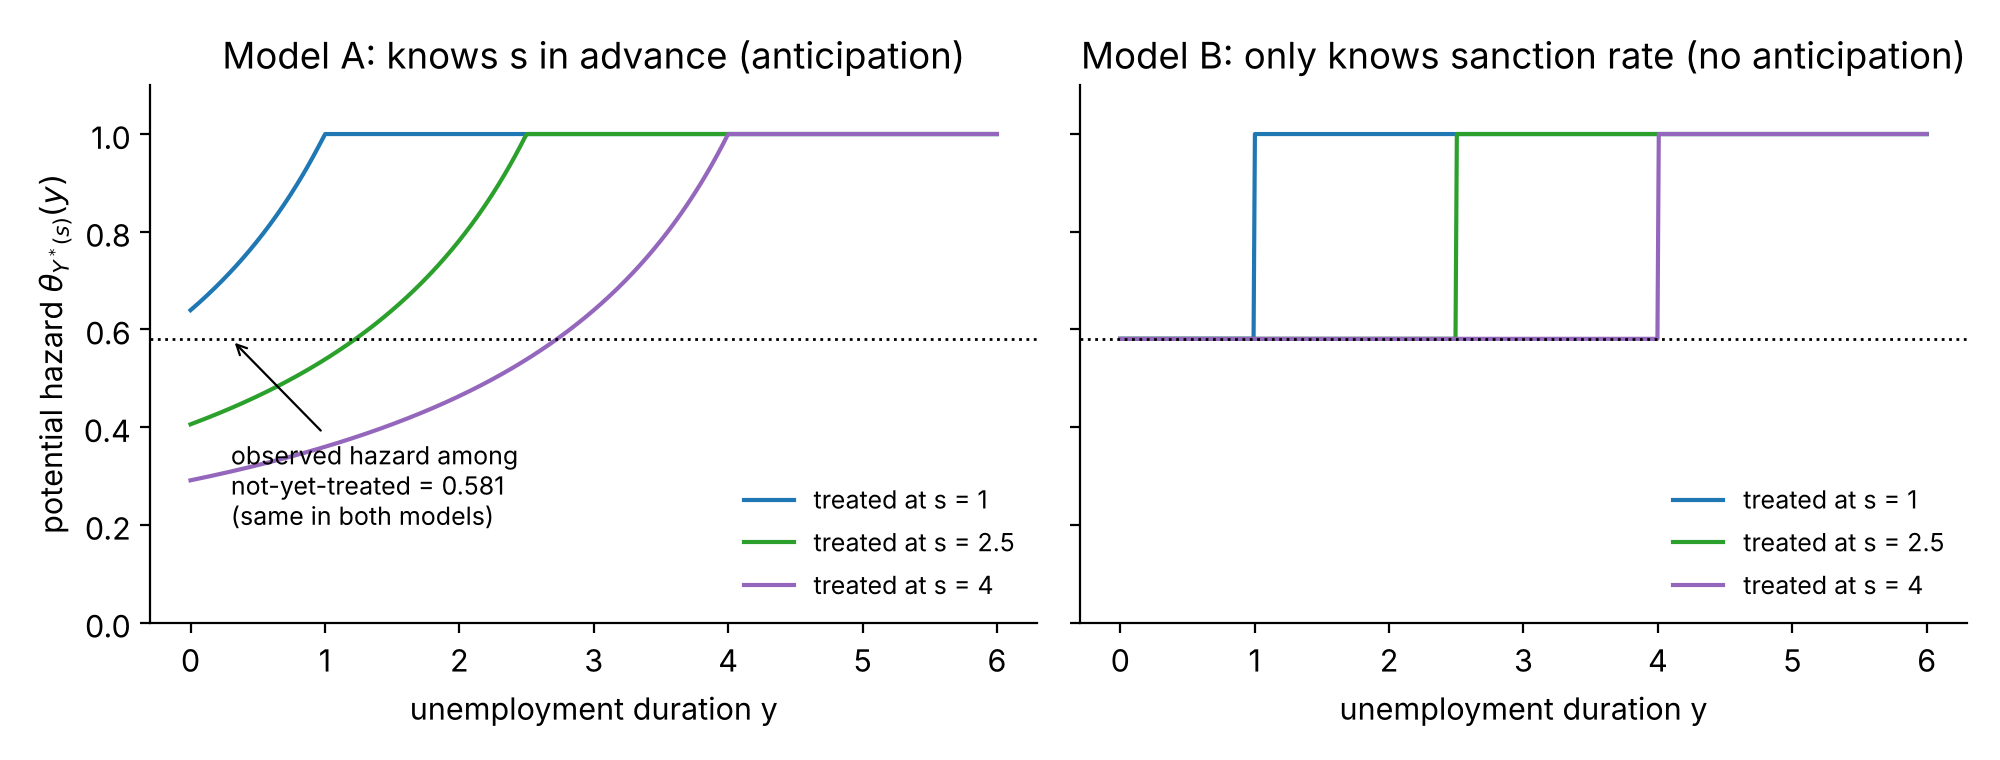
\includegraphics[width=0.82\linewidth]{fig2_anticipation_equivalence.png}

  \raggedright\small
  Model A: the worker knows the sanction date $s$, and search effort (hence the hazard) rises before $s$. Model B: only the sanction rate is known, so the hazard jumps at $s$. With suitably chosen parameters the two produce \emph{identical} data. The data only reveal the hazard among the not-yet-treated (0.581 in both).

  \smallskip
  \textbf{Proof of Prop.~1.} By Tsiatis/Miller there is an independent pair $(\hat Y,\hat S)$ matching the competing-risks part. Use $\hat S$ as the treatment and $\hat Y$'s hazard before treatment for every $Y^*(s)$; define post-treatment hazards from $P_1$.
\note{
Parameters: $w=1$, $b=1/2$. Model A has a discount rate of 5\%; Model B has a discount rate of 1.23\% and a sanction rate of 0.419. Equation (3) of the paper gives Model A's hazard; footnote 11 derives the common observed hazard.
}
\end{frame}

\begin{frame}{Appendix B: data objects vs.\ the paper's $(Q_S,Q_Y)$}
  The paper's data: $Q_S(y,s)=\Pr(Y>y,S>s,Y>S)$ and $Q_Y(y)=\Pr(Y>y,Y<S)$. Then
  \begin{align*}
    P_0(t)&=Q_S(t,t)+Q_Y(t),\\
    h_Y(t)&=-Q_Y'(t)/P_0(t),\qquad h_S(t)=-\partial_sQ_S(t,s)\big|_{s=t}\big/P_0(t),\\
    P_1(y\mid s)&=\partial_sQ_S(y,s)\big/\partial_sQ_S(s,s)\qquad(y>s).
  \end{align*}
  Conversely, $(P_0,h_Y,h_S,P_1)$ determine $(Q_S,Q_Y)$. The objects are equivalent.
\end{frame}

\begin{frame}{Appendix C: uniqueness in step 3}
  Suppose $(a,b)\neq(a',b')$ both satisfy $P_0(t\mid x)=\Lap(\varphi_Y(x)a,\varphi_S(x)b)$ for all $x$. Then $\Lap(pa,qb)=\Lap(pa',qb')$ on an open set of $(p,q)$. By analyticity,
  \[ \Lap(u,v)=\Lap(ku,mv)\quad\text{for all }(u,v)\in(0,\infty)^2,\qquad k=a'/a,\ m=b'/b,\ (k,m)\neq(1,1). \]
  \begin{itemize}
    \item $k,m\ge1$ (or both $\le1$): contradicts $\Lap$ strictly decreasing in each argument (needs $\Pr(V\in(0,\infty)^2)>0$).
    \item $k>1>m$: iterating gives $\Lap(u,v)=\Lap(k^nu,m^nv)\to\Pr(V_Y=0)$ as $n\to\infty$. So $\Lap$ is constant, a contradiction. The case $k<1<m$ is symmetric.
  \end{itemize}
\end{frame}

\begin{frame}{Appendix D: proof sketches for Models 1b, 2a, 2b}
  \small
  \textbf{Model 1b (Prop.~4).} After Prop.~2, for $y>s$:
  \[ \frac{\partial^2Q_S(y,s\mid x)/\partial y\partial s}{\partial^2Q_S(y,s\mid x^*)/\partial y\partial s}\;\xrightarrow{\;y,s\downarrow0\;}\;\varphi_S(x)\varphi_\Delta(x) \quad(\text{needs }\E[V_\Delta V_S]<\infty), \]
  which identifies $\varphi_\Delta$. Then $\partial_sQ_S/(\lambda_S\varphi_S)=\Lap^{(S)}_{G_\Delta}\big(\varphi_Y\Lambda_Y(s),\varphi_\Delta(\Lambda_\Delta(y)-\Lambda_\Delta(s)),\varphi_S\Lambda_S(s)\big)$. Let $s\downarrow0$ to get $\Lambda_\Delta$; vary $x,y$ to trace $\Lap_{G_\Delta}$ on an open set.

  \medskip
  \textbf{Models 2a/2b (Prop.~5).} Two spells per stratum sharing $V=(V_Y,V_S)$ (or $(V_Y,V_\Delta,V_S)$), spell-specific baselines and effects. The two-spell competing-risks structure identifies $\Lambda_{Y_k},\Lambda_{S_k}$ (Abbring \& Van den Berg 2003, JRSSB). The extra cross-spell information then identifies $\delta_k$ and $G$, \textbf{without covariates and without finite means}, mirroring Honoré (1993).
\end{frame}

\end{document}
"
% (or just run ./build.sh)
\documentclass[aspectratio=169,10pt]{beamer}
\ifdefined\withnotes
  \setbeameroption{show notes}
\fi
\setbeamertemplate{navigation symbols}{}
\setbeamertemplate{footline}[frame number]
\setbeamertemplate{note page}{\vspace{1em}\small\insertnote}

\usepackage{amsmath,amssymb,booktabs,tikz}
\usetikzlibrary{arrows.meta,positioning}
\graphicspath{{../figures/}}

\newcommand{\E}{\mathbb{E}}
\newcommand{\1}{\mathbf{1}}
\newcommand{\R}{\mathbb{R}}
\newcommand{\Lap}{\mathcal{L}}
\newcommand{\cov}{\operatorname{Cov}}

\title{The Nonparametric Identification of Treatment Effects in Duration Models}
\subtitle{Abbring \& Van den Berg (2003, \textit{Econometrica})}
\author{Econometrics Reading Group}
\date{}

\begin{document}

% =====================================================================
\begin{frame}
  \titlepage
\note{
\textbf{How to read these notes.} Every slide has a note like this one. The notes say where the slide's content comes from, what the previous slide left unresolved, and what this slide adds. Read slides + notes in order: the argument is cumulative.

\medskip
\textbf{The plan in one sentence.} We want the effect of a treatment that arrives at a random time during a spell. The difficulty is selection on unobservables. The paper's answer is that the \emph{pre-treatment} part of the data is a competing-risks problem; with hazard structure, that part reveals the distribution of unobserved types among those at risk; knowing that distribution lets us strip the selection out of the \emph{post-treatment} part.

\medskip
\textbf{Notation changes relative to the paper.} We write the data as four interpretable objects ($P_0, h_Y, h_S, P_1$) instead of the paper's sub-survival functions $(Q_S,Q_Y)$; the mapping is in the appendix. We write $D(y\mid s,x)$ for the integrated post-treatment hazard (the paper uses $\Upsilon$). We write the bivariate Laplace transform as $\Lap(a,b)$ and its partial derivatives as $\Lap_a,\Lap_b,\Lap_{ab}$.
}
\end{frame}

% =====================================================================
\begin{frame}{The question}
  \textbf{Running example.} An unemployed worker may receive a benefit sanction at a random time $S$ during the spell. Outcome: unemployment duration $Y$.

  \medskip
  \textbf{Target.} The causal effect of the sanction on the \emph{exit rate} to work.

  \medskip
  \textbf{Why this is hard}
  \begin{enumerate}
    \item \textbf{Dynamic treatment:} no fixed treated group; everyone is untreated until $S$.
    \item \textbf{Treatment is censored:} if you find a job before your sanction date, $S$ is never seen.
    \item \textbf{Selection on unobservables:} low-motivation workers get sanctioned earlier \emph{and} exit more slowly.
    \item \textbf{No credible instrument:} whatever shifts sanctions, the worker likely sees and reacts to.
  \end{enumerate}

  \medskip
  \textbf{Punchline.} The \emph{timing} of $S$ relative to $Y$ does the job of the instrument, at the price of structure on hazards.
\note{
Point 4 is the paper's own argument (Section 1) against IV. If a variable affects treatment and the agent can see it, a forward-looking agent adjusts behaviour, so the variable also affects the outcome hazard directly. Exclusion restrictions are therefore hard to defend in dynamic settings.

Point 2 explains why the data are unusual. We see $S$ only for people with $S<Y$. This censoring is not a nuisance to be fixed; it is what turns the pre-treatment data into a competing-risks problem (slide 10).

The punchline is what the rest of the talk earns. Keep the four difficulties visible: each later assumption addresses one of them.
}
\end{frame}

% =====================================================================
\begin{frame}{Primer 1: hazards and dynamic selection}
  \begin{columns}[T]
    \begin{column}{0.47\textwidth}
      \textbf{Hazard} of a duration $T$:
      \[ \theta(t)=\lim_{dt\downarrow0}\tfrac{\Pr(T\in[t,t+dt)\mid T\ge t)}{dt} \]
      $\Lambda(t)=\int_0^t\theta$, \quad $\Pr(T>t)=e^{-\Lambda(t)}$.

      \smallskip
      In every instant, each survivor flips a coin with success probability $\theta(t)\,dt$.

      \medskip
      \textbf{Heterogeneity:} $\theta(t\mid V)=\lambda(t)\,V$. Then the hazard we \emph{observe} is
      \[ \bar\theta(t)=\lambda(t)\;\E[V\mid T\ge t], \]
      and $\E[V\mid T\ge t]$ \textbf{falls}: high-$V$ people leave first.
    \end{column}
    \begin{column}{0.53\textwidth}
      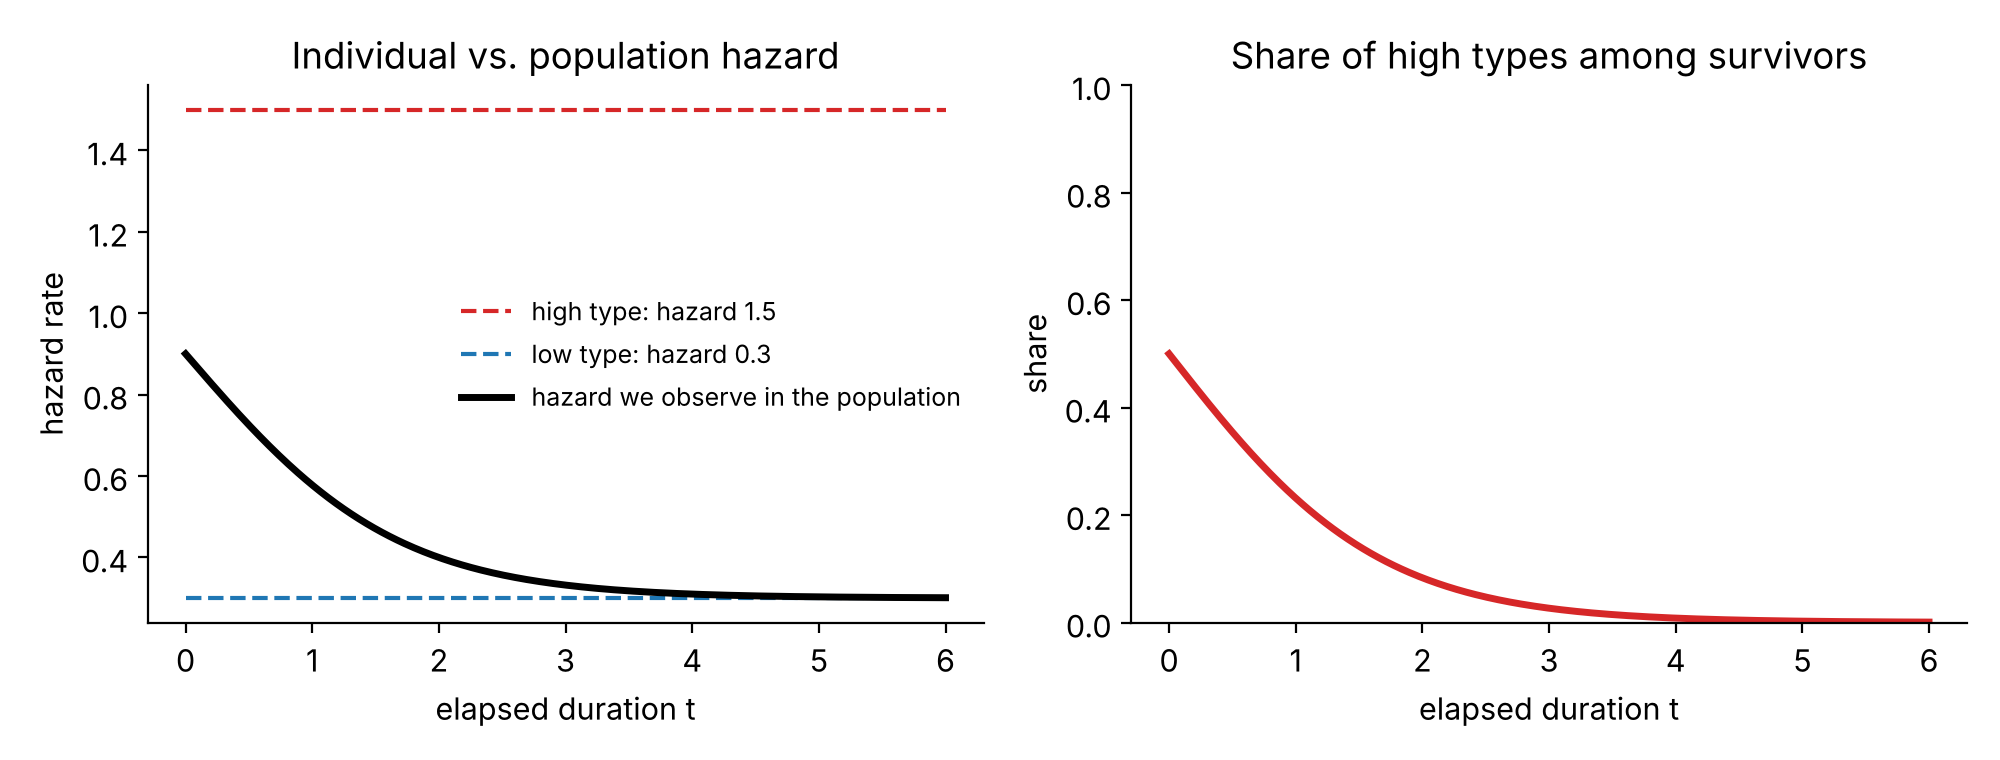
\includegraphics[width=\linewidth]{fig1_dynamic_selection.png}
    \end{column}
  \end{columns}

  \medskip
  \textbf{Trap or sorting?} A falling exit rate can be true duration dependence ($\lambda\downarrow$) or composition ($\E[V\mid T\ge t]\downarrow$). This is Heckman's \emph{true vs.\ spurious state dependence}, in continuous time.
\note{
\textbf{Derivation of the observed hazard.} The survival function is $\Pr(T>t)=\E[e^{-V\Lambda(t)}]$, with $\Lambda(t)=\int_0^t \lambda$. The population hazard is $-\frac{d}{dt}\log\Pr(T>t)=\lambda(t)\,\E[Ve^{-V\Lambda(t)}]/\E[e^{-V\Lambda(t)}]$. The ratio is the mean of $V$ under weights $e^{-V\Lambda(t)}$, i.e.\ $\E[V\mid T\ge t]$. The weight $e^{-V\Lambda(t)}$ is the probability that a type-$V$ person is still there. That is the whole idea of dynamic selection.

\textbf{Why it matters for treatment effects.} The people still unemployed and untreated at month 6 are a selected group. Comparing ``treated at month 6'' with ``not yet treated at month 6'' is only valid if we know how both groups were selected up to month 6. Every identification step below is about learning that selection.

\textbf{Figure.} Two types with \emph{constant} hazards 0.3 and 1.5 produce a population hazard that falls from 0.9 to 0.3. Nobody's hazard changes; only the composition does.

\textbf{The coin-flip view} matters later. Conditional on the hazard, the moment of the event is pure chance. This is the source of the ``randomization'' the paper exploits (footnote 15).
}
\end{frame}

% =====================================================================
\begin{frame}{Primer 2: the MPH model and the Laplace-transform toolkit}
  \textbf{Mixed proportional hazard:} $\theta(t\mid x,V)=\lambda(t)\,\varphi(x)\,V$, \quad $V\sim G$, \ $V\perp x$. Then
  \[ \Pr(T>t\mid x)=\E\big[e^{-V\varphi(x)\Lambda(t)}\big]=\Lap\big(\varphi(x)\Lambda(t)\big),\qquad \Lap(a):=\E[e^{-aV}]. \]
  \textbf{Toolkit.} $e^{-aV}$ is the probability that type $V$ survives to index $a$. So derivatives of $\log\Lap$ are \emph{moments among survivors}. In two dimensions, $\Lap(a,b)=\E[e^{-aV_Y-bV_S}]$:
  \[
    -\partial_a\log\Lap=\E[V_Y\mid\text{surv.}],\qquad
    -\partial_b\log\Lap=\E[V_S\mid\text{surv.}],\qquad
    \partial^2_{ab}\log\Lap=\cov(V_Y,V_S\mid\text{surv.}).
  \]
  \textbf{Single-risk identification (Elbers \& Ridder 1982), in 3 steps}
  \begin{enumerate}
    \item $t\downarrow0$: nobody has been selected out yet, so hazard ratios across $x$ give $\varphi(x)$ (needs $\E V<\infty$).
    \item At $t^*$ with $\Lambda(t^*)=1$: $\Pr(T>t^*\mid x)=\Lap(\varphi(x))$. Varying $x$ traces $\Lap$, hence $G$.
    \item Any $t$: solve $\Pr(T>t\mid x)=\Lap(\varphi(x)\Lambda(t))$ for $\Lambda(t)$.
  \end{enumerate}
  \textbf{We will run exactly this logic in two dimensions.}
\note{
\textbf{Where the toolkit comes from.} $\log\Lap(a,b)$ is the cumulant generating function of $(-V_Y,-V_S)$, evaluated under tilting by $e^{-aV_Y-bV_S}$. First derivative: $\partial_a\log\Lap=-\E[V_Ye^{-aV_Y-bV_S}]/\Lap=-\E_w[V_Y]$. Differentiate again in $b$: $\partial_b(-\E_w[V_Y])=\E_w[V_YV_S]-\E_w[V_Y]\E_w[V_S]=\cov_w(V_Y,V_S)$. The weights $w$ are survival probabilities, so ``$\E_w$'' means ``among survivors''. Two consequences we use repeatedly:
(i) the observed hazard is $\lambda\varphi\times(-\partial_a\log\Lap)$;
(ii) the dependence between $V_Y$ and $V_S$ among survivors (the selection) is a cross-derivative.

\textbf{Step 1 in detail.} The hazard is $\lambda(t)\varphi(x)\E[V\mid T\ge t,x]$. As $t\downarrow0$, $\E[V\mid T\ge t,x]\to\E[V]$, which is finite by assumption and the same for all $x$ because $V\perp x$. The ratio across $x$ and $x^*$ therefore tends to $\varphi(x)/\varphi(x^*)=\varphi(x)$. Note that identification uses the behaviour of short durations, where data are thin (critique on slide 17).

\textbf{Step 2.} The normalization $\Lambda(t^*)=1$ fixes the scale. Once $\varphi$ is known, $x\mapsto\Pr(T>t^*\mid x)$ is $\Lap$ evaluated at known points. Varying $x$ traces $\Lap$ on an interval. Laplace transforms are analytic, so $\Lap$ is then pinned down everywhere, and it determines $G$ uniquely.

\textbf{Step 3.} $\Lap$ is strictly decreasing, so invert.
}
\end{frame}

% =====================================================================
\begin{frame}{Set-up: potential outcomes indexed by treatment time}
  \begin{itemize}
    \item Treatments are dates $s\in[0,\infty]$ ($s=\infty$: never). Potential outcomes $Y^*(s)$; observed $Y=Y^*(S)$.
    \item \textbf{No anticipation:} $\theta_{Y^*(s)}(t)=\theta_{Y^*(s')}(t)$ for $t\le\min(s,s')$. A future treatment date does not affect today's hazard.\\
      Reacting to the sanction \emph{regime} is allowed (it is in every $Y^*(s)$), so the effect is \emph{``treated at $s$ vs.\ later, under this regime''}.
  \end{itemize}
  \begin{center}
  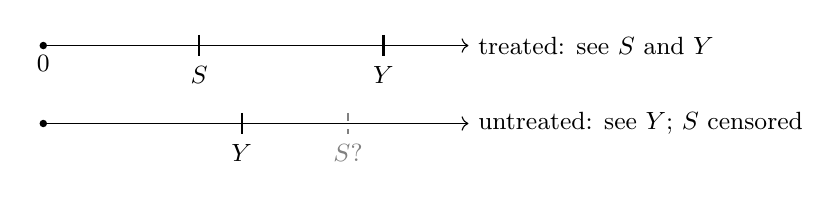
\begin{tikzpicture}[scale=0.9]
    \draw[->] (0,0) -- (6,0) node[right] {\small treated: see $S$ and $Y$};
    \fill (0,0) circle (1.5pt) node[below] {\small 0};
    \draw[thick] (2.2,0.15) -- (2.2,-0.15) node[below] {\small $S$};
    \draw[thick] (4.8,0.15) -- (4.8,-0.15) node[below] {\small $Y$};
    \draw[->] (0,-1.1) -- (6,-1.1) node[right] {\small untreated: see $Y$; $S$ censored};
    \fill (0,-1.1) circle (1.5pt);
    \draw[thick] (2.8,-0.95) -- (2.8,-1.25) node[below] {\small $Y$};
    \draw[dashed,gray] (4.3,-0.95) -- (4.3,-1.25) node[below] {\small $S$?};
  \end{tikzpicture}
  \end{center}
  \textbf{What the data reveal} (all conditional on $x$):
  \begin{itemize}
    \item $P_0(t)=\Pr(Y>t,S>t)$: nothing has happened by $t$;
    \item $h_Y(t)$, $h_S(t)$: rate of exiting untreated / of being treated, among those with nothing yet;
    \item $P_1(y\mid s)=\Pr(Y>y\mid S=s,\,Y>s)$: post-treatment survival of the \textbf{cohort treated at $s$}.
  \end{itemize}
  \textbf{Fact (Prop.~1):} any such data can be rationalized with no anticipation \emph{and} random assignment. So no anticipation is untestable, and we need a model of selection.
\note{
\textbf{Why index potential outcomes by a date.} A dynamically assigned binary treatment is really a continuum of mutually exclusive treatments, ``treated at $s$''. This is exactly the staggered-adoption set-up, where potential outcomes are indexed by the adoption cohort $g$ (slide 18).

\textbf{No anticipation.} The paper states it for integrated hazards; hazard paths agreeing up to $\min(s,s')$ is the same thing. In biostatistics this is a mild consistency condition. In economics it is behavioural: if a worker knows the sanction date and searches harder beforehand, it fails. If information arrives before treatment, the paper suggests treating the \emph{information shock} as the treatment.

\textbf{The data objects.} These four objects are equivalent to the paper's $(Q_S,Q_Y)$; see the appendix. The pre-treatment objects ($P_0,h_Y,h_S$) are classic \emph{competing-risks} data: two things can happen and we see which happens first. $P_1$ is the only place where the treatment effect can appear.

\textbf{Proposition 1 (de-emphasized).} By the Tsiatis/Miller result, any competing-risks data are generated by some \emph{independent} pair of latent durations. Use that pair for the pre-treatment part, and define the post-treatment hazard to match $P_1$. The result is a model with random assignment and no anticipation that fits the data perfectly. Two lessons: selection cannot be told from causality without structure, and anticipation cannot be detected. The paper's job-search illustration is in the appendix.
}
\end{frame}

% =====================================================================
\begin{frame}{The model}
  \textbf{Assumption 2 (selection on $(x,V)$):} $Y^*(\cdot)\perp S \mid (x,V)$, with $V$ time-invariant.

  \medskip
  \textbf{Model 1a.}
  \[
  \theta_Y(t\mid s,x,V)=\lambda_Y(t)\,\varphi_Y(x)\,V_Y\cdot\delta(t\mid s,x)^{\1\{t>s\}},\qquad
  \theta_S(t\mid x,V)=\lambda_S(t)\,\varphi_S(x)\,V_S,
  \]
  with $(V_Y,V_S)\sim G$ \textbf{arbitrarily dependent}, independent of $x$.

  \medskip
  \begin{itemize}
    \item Two MPH hazards. Their link through $\cov(V_Y,V_S)$ is the \textbf{selection on unobservables}.
    \item $\delta$ is the \textbf{causal effect}: a hazard multiplier after treatment. It may vary with $t$, $s$ (hence with $t-s$) and $x$, but not with $V$.
    \item No anticipation is built in: $\delta$ only acts for $t>s$.
    \item The same $x$ enters both hazards, so there is \textbf{no exclusion restriction}. $\lambda$'s, $\varphi$'s, $G$, $\delta$ are all nonparametric.
  \end{itemize}

  \medskip
  \textbf{Assn.~3:} $\{(\varphi_Y(x),\varphi_S(x))\}$ contains an open set of $\R^2$. \quad \textbf{Assn.~4:} $\E V_Y,\E V_S<\infty$.\\
  Normalizations: $\varphi(x^*)=1$, $\Lambda(t^*)=1$.
\note{
\textbf{How the model emerges from the set-up.} No anticipation says pre-treatment hazards do not depend on $s$. Assumption 2 says all dependence between $Y$ and $S$ runs through $(x,V)$. Together they imply: conditional on $(x,V)$, $Y$ and $S$ are linked \emph{only} through the causal factor $\delta$. That is why $\delta$ can be called a treatment effect.

\textbf{Why hazard-based assignment matters.} $S$ is modelled by a hazard, not by a threshold-crossing rule. So even conditional on $(x,V)$, $S$ is random: $\varphi_S(x)V_S\Lambda_S(S)$ is a unit exponential independent of $(x,V)$. This random component moves $S$ around without affecting $Y$ except through treatment. It is the analogue of an instrument (slide 8).

\textbf{Assumption 3 is not an exclusion restriction, but it is not free.} The covariates must move the two hazards \emph{non-proportionally}. With $\varphi_j(x)=e^{x'\beta_j}$ you need at least two continuous covariates and $(\beta_Y\ \beta_S)$ of full rank.

\textbf{Allowed but not shown:} mass points of $V$ at zero (never treated / never exit). Also $\Pr(Y=S)=0$ (continuous time, no ties).
}
\end{frame}

% =====================================================================
\begin{frame}{The selection problem at the moment of treatment}
  Fix a duration $s$. Write $a_s=\varphi_Y(x)\Lambda_Y(s)$, $b_s=\varphi_S(x)\Lambda_S(s)$.

  \medskip
  \textbf{Who is still at risk} (nothing happened by $s$):\quad $dG_{R_s}(v)\propto e^{-a_s v_Y-b_s v_S}\,dG(v)$.\\[2pt]
  \textbf{Who is treated at $s$:} the risk set, reweighted by the treatment intensity, \quad $dG_{s}(v)\propto v_S\,dG_{R_s}(v)$.

  \medskip
  \textbf{Exit hazards right at $s$:}
  \[
  \underbrace{\lambda_Y(s)\varphi_Y(x)\,\E_{R_s}[V_Y]}_{\text{not yet treated}}
  \qquad\text{vs.}\qquad
  \underbrace{\lambda_Y(s)\varphi_Y(x)\,\delta(s\mid s,x)\,\E_{s}[V_Y]}_{\text{just treated}}
  \]
  \[
  \frac{\text{just treated}}{\text{not yet treated}}
  \;=\;\delta(s\mid s,x)\times\underbrace{\Big(1+\frac{\cov_{R_s}(V_Y,V_S)}{\E_{R_s}[V_Y]\,\E_{R_s}[V_S]}\Big)}_{\text{selection factor}}
  \]
  \begin{itemize}
    \item If $V_Y\perp V_S$ among survivors, timing is as good as random at $s$: the ratio \emph{is} the causal effect.
    \item Otherwise we need the \textbf{joint distribution of types among survivors}. The pre-treatment data will supply it.
  \end{itemize}
\note{
\textbf{This slide is the heart of the paper's logic.} It reduces the selection problem to one object.

\textbf{Derivation.} Being at risk at $s$ means $Y>s$ and $S>s$. Given $V$, no anticipation means $Y$'s hazard before $s$ is the untreated one, so the probability of being at risk is $e^{-a_sV_Y}e^{-b_sV_S}$ (Assumption 2 lets the two terms multiply). By Bayes' rule, the type distribution in the risk set is $G$ reweighted by that probability. Among those at risk, the chance of being treated in $[s,s+ds)$ is $\lambda_S(s)\varphi_S(x)V_S\,ds$. So the treated cohort is the risk set reweighted by $V_S$.

The mean of $V_Y$ in the treated cohort is
$\E_s[V_Y]=\E_{R_s}[V_YV_S]/\E_{R_s}[V_S]=\E_{R_s}[V_Y]+\cov_{R_s}(V_Y,V_S)/\E_{R_s}[V_S]$.
Divide by $\E_{R_s}[V_Y]$ to get the selection factor.

\textbf{Reading it.} Suppose low-motivation people (low $V_Y$) are sanctioned more (high $V_S$), so the covariance is negative. Then the just-treated have low $V_Y$, and the naive comparison \emph{understates} a positive effect of sanctions on exit. This is the classic ``Heckman selection'' structure, with a control-function-like correction factor.

\textbf{The ratio on the left is data.} The hazard of the just-treated is $-\partial_y\log P_1(y\mid s)$ as $y\downarrow s$; the hazard of the not-yet-treated is $h_Y(s)$. So everything hinges on the selection factor, a feature of the joint distribution of $(V_Y,V_S)$ among those at risk at $s$.
}
\end{frame}

% =====================================================================
\begin{frame}{Timing as an instrument}
  \footnotesize
  \begin{tabular}{p{0.2\textwidth}p{0.29\textwidth}p{0.41\textwidth}}
    \toprule
    & Static selection / IV & Timing of events \\
    \midrule
    Exogenous variation in treatment
    & excluded variable $Z$
    & the timing shock: given $(x,V)$, $S=\Lambda_S^{-1}\!\big(\tfrac{E_S}{\varphi_S(x)V_S}\big)$, $E_S\sim\text{Exp}(1)$ \\[3pt]
    What is excluded from the outcome
    & the \emph{variable} $Z$
    & the \emph{shock} $E_S$ (via Assn.~2) \\[3pt]
    Correcting for who selects in
    & control function $\E[U\mid D=1,Z]$
    & selection factor / $G_s$, from the competing-risks data \\[3pt]
    Covariate requirement
    & $Z$ shifts $D$, not $Y$
    & $x$ shifts both hazards, \emph{non-proportionally} (Assn.~3) \\
    \bottomrule
  \end{tabular}

  \normalsize
  \bigskip
  \textbf{Why timing is informative.} The treatment acts only \emph{after} $S$; $V$ acts \emph{throughout}.
  \begin{itemize}
    \item Causal effect $\Rightarrow$ \textbf{local} dependence: exits bunch right after $S$, \emph{whenever} $S$ occurs.
    \item Selection $\Rightarrow$ \textbf{global} dependence: early-treated people are early leavers in general.
  \end{itemize}
  In a static latent-index model the treatment effect needs an exclusion restriction. Here the timing replaces it.
\note{
\textbf{The point of the table.} An IV design needs two things: (i) variation in treatment that is unrelated to the outcome's unobservables, and (ii) a way to handle the fact that the people who take treatment are selected.

(i) In a static threshold model $D=\1\{\mu(Z)>U\}$, treatment is deterministic given $(Z,U)$, so exogenous variation must come from an excluded $Z$. With hazard-based assignment, treatment \emph{timing} is still random given $(x,V)$. The representation uses the fact that $\varphi_S(x)V_S\Lambda_S(S)$ is unit exponential. The exclusion restriction has not disappeared: it moved from an observed variable to an unobserved shock. Assumption 2 says the timing shock $E_S$ is independent of everything that drives $Y$. Be candid about this in the talk.

(ii) The selection correction is the analogue of a control function. Here it is not estimated from an excluded instrument; it comes from the competing-risks part of the data (next three slides).

\textbf{Local vs.\ global.} This is the paper's own intuition (Section 3.2) and the basis of the companion paper on testing the sign of $\delta$. The figure on the next slide makes it concrete.
}
\end{frame}

% =====================================================================
\begin{frame}{What the data look like}
  \centering
  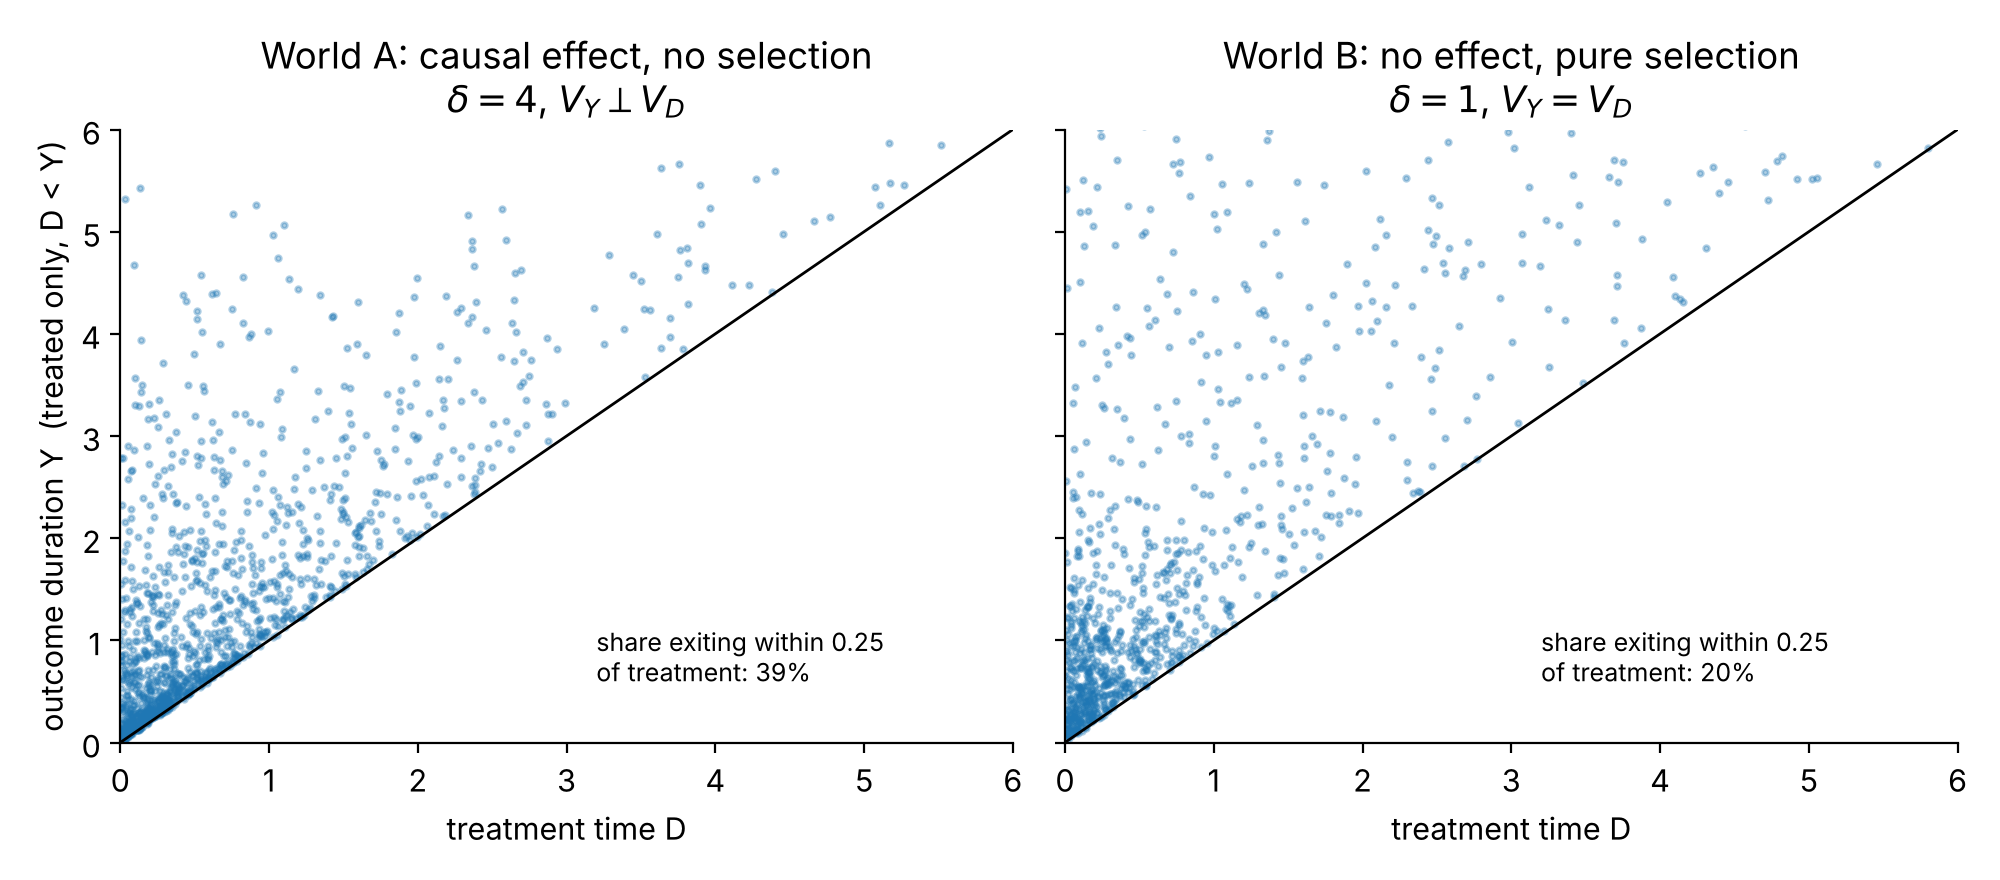
\includegraphics[width=0.85\linewidth]{fig3_local_vs_global.png}

  \raggedright\small
  Treated observations only. Left: $\delta=4$, independent frailties. Right: $\delta=1$, $V_Y=V_S$. A causal effect makes points hug the diagonal \emph{at every $S$}. Selection produces quick exits only where high types are concentrated (small $S$).
\note{
\textbf{Simulation.} Two types (0.25 and 2), constant baseline hazards. World A: types for $Y$ and $S$ drawn independently, and treatment multiplies the exit hazard by 4. World B: one common type, no effect.

Both worlds show a positive association between $S$ and $Y$, and in both some people exit quickly after treatment. The difference is \emph{where} the quick exits are. In A they occur after treatment at any $S$; in B they are concentrated at small $S$, where the high types still are. The formal argument quantifies exactly this: how many quick post-treatment exits would we expect from selection alone, given the types at risk at $s$?

Script: \texttt{figures/make\_figures.py}.
}
\end{frame}

% =====================================================================
\begin{frame}{The pre-treatment data are a competing-risks problem}
  Before treatment there are two latent clocks: $Y^0$ (exit if never treated) and $S$. Their joint survival is
  \[ \Pr(Y^0>y,\,S>s\mid x)=\Lap\big(\varphi_Y(x)\Lambda_Y(y),\;\varphi_S(x)\Lambda_S(s)\big). \qquad \text{($\delta$ does not appear!)}\]
  We only see the \emph{first} event: the diagonal $y=s=t$, i.e.\ $P_0(t\mid x)=\Lap(a_t(x),b_t(x))$, plus which event it was.

  \smallskip
  \textbf{Tsiatis (1975):} without structure, any such data are generated by \emph{independent} clocks. The dependence, i.e.\ the selection, is unidentified.

  \begin{center}
    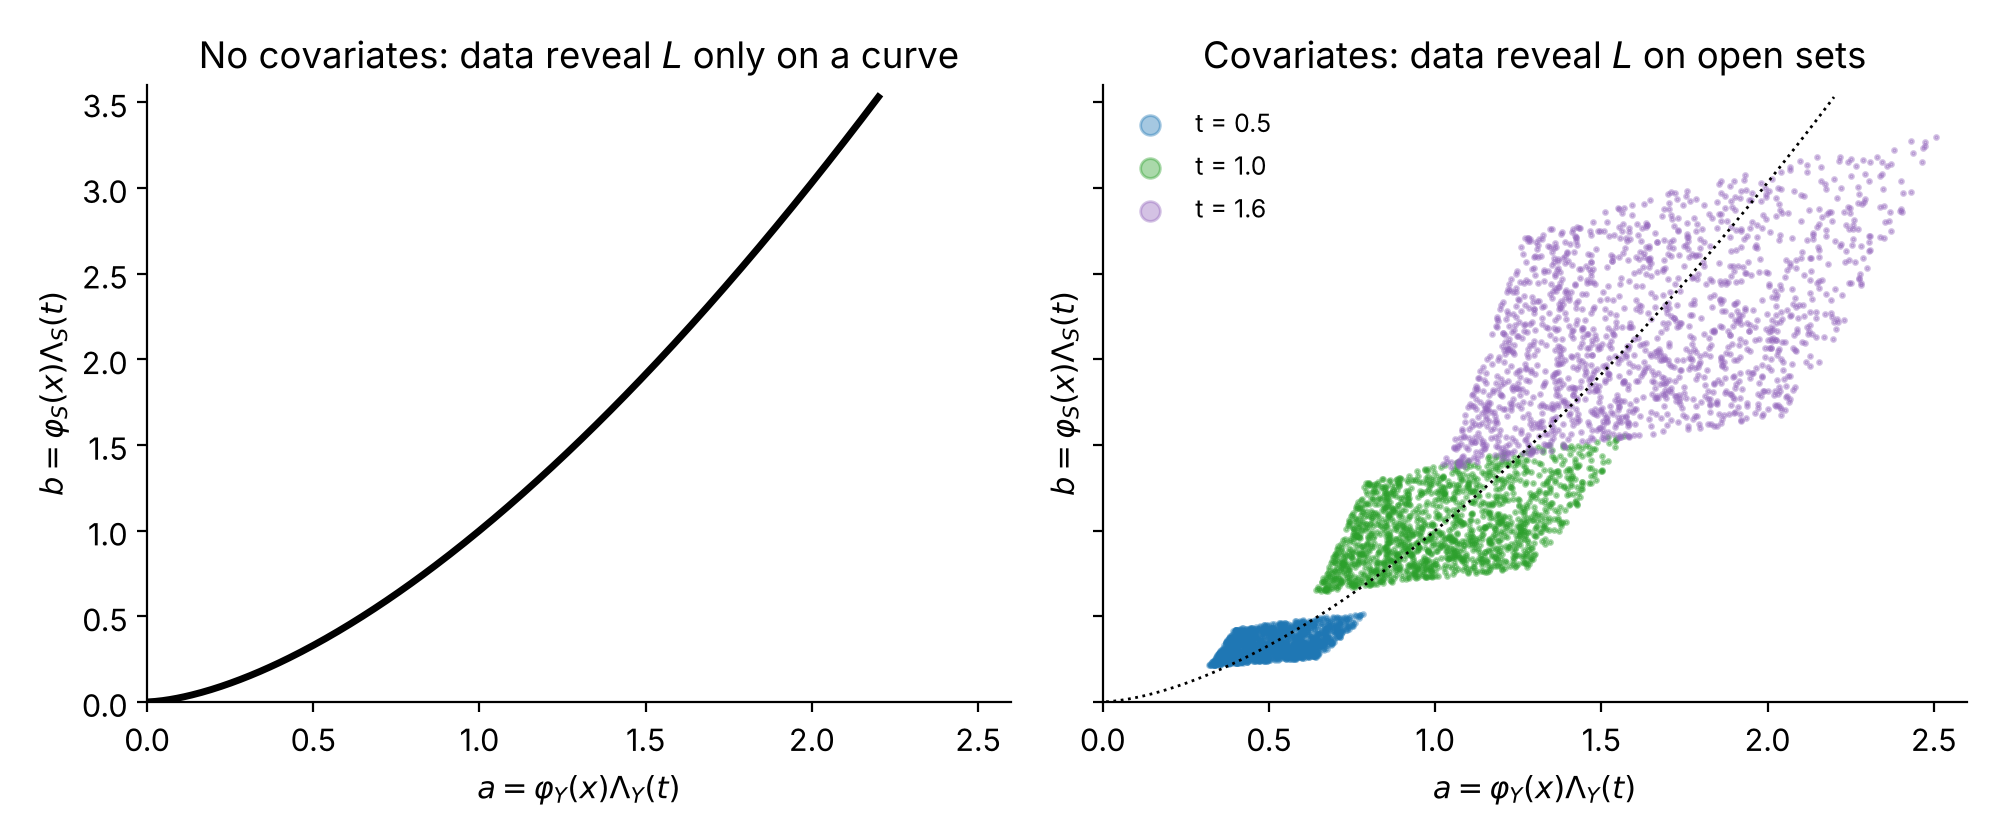
\includegraphics[width=0.56\linewidth]{fig4_competing_risks_geometry.png}
  \end{center}
  \vspace{-6pt}
  \small Without $x$, the data reveal $\Lap$ only along a curve $t\mapsto(\Lambda_Y(t),\Lambda_S(t))$. A curve cannot pin down a function of two variables. With $x$ shifting the two hazards separately, the data reveal $\Lap$ on \emph{open sets}.
\note{
\textbf{Why this is the crucial step.} Slide 7 showed that everything hinges on the joint distribution of $(V_Y,V_S)$. The only place to learn it without using the outcome we want to explain is the pre-treatment period. There, by no anticipation, nothing causal is going on. We just watch two clocks race.

\textbf{The joint survival.} Given $V$, the two clocks are independent with integrated hazards $\varphi_Y\Lambda_YV_Y$ and $\varphi_S\Lambda_SV_S$. Integrating over $G$ gives the bivariate Laplace transform evaluated at the two indices.

\textbf{Geometry of non-identification.} With no covariates, data at duration $t$ tell us $\Lap$ at one point $(\Lambda_Y(t),\Lambda_S(t))$. As $t$ varies we learn $\Lap$ along a curve, plus the slopes of $\Lap$ in the two directions along that curve (from the cause-specific hazards). Many bivariate distributions agree on those values, including independent ones. That is Tsiatis' result.

\textbf{How covariates break it.} At a fixed $t$, varying $x$ moves the point to $(\varphi_Y(x)\Lambda_Y(t),\varphi_S(x)\Lambda_S(t))$. If the two $\varphi$'s move independently (Assumption 3), the point sweeps out a two-dimensional patch. Knowing an analytic function on any open patch determines it everywhere. This is why Assumption 3 must be two-dimensional, and it is what makes the selection identified.
}
\end{frame}

% =====================================================================
\begin{frame}{Identifying the competing-risks part (Prop.~2): three steps}
  \textbf{Step 1: $\varphi$'s from short durations} (nobody has been selected out yet):
  \[ \frac{h_Y(t\mid x)}{h_Y(t\mid x^*)}=\frac{\varphi_Y(x)\,\E[V_Y\mid R_t,x]}{\E[V_Y\mid R_t,x^*]}\;\xrightarrow{\;t\downarrow0\;}\;\varphi_Y(x),\qquad\text{same for }\varphi_S. \]
  Uses \emph{which} event happened and $\E V<\infty$.

  \medskip
  \textbf{Step 2: $G$ at the normalization date} ($\Lambda_Y(t^*)=\Lambda_S(t^*)=1$):
  \[ P_0(t^*\mid x)=\Lap\big(\varphi_Y(x),\varphi_S(x)\big). \]
  Known points fill an open set (Assn.~3), so $\Lap$ is known there. $\Lap$ is real-analytic, so it is known on $(0,\infty)^2$, and $\Lap$ determines $G$, \textbf{including the dependence between $V_Y$ and $V_S$}.

  \medskip
  \textbf{Step 3: baselines.} For every $t$, $(\Lambda_Y(t),\Lambda_S(t))$ is the unique $(a,b)$ with
  \[ P_0(t\mid x)=\Lap\big(\varphi_Y(x)\,a,\;\varphi_S(x)\,b\big)\quad\text{for all }x. \]

  \medskip
  $\Rightarrow$ $\lambda_Y,\lambda_S,\varphi_Y,\varphi_S,G$ are identified \textbf{without touching post-treatment data}.
\note{
\textbf{Relation to the paper.} The paper proves Proposition 2 by citing Abbring \& Van den Berg (2003, JRSSB). The three steps here are a self-contained route that makes the logic visible. It is Elbers--Ridder (slide 4) in two dimensions.

\textbf{Step 1.} The cause-specific hazard of exiting untreated among those at risk is $h_Y(t\mid x)=\lambda_Y(t)\varphi_Y(x)\E[V_Y\mid R_t,x]=\lambda_Y(t)\varphi_Y(x)\big(-\partial_a\log\Lap\big)(a_t,b_t)$. As $t\downarrow0$ the risk set is the whole population. Because $V\perp x$ and $\E V_Y<\infty$, the conditional mean tends to the same constant for all $x$, and $\lambda_Y(t)$ cancels in the ratio.

\textbf{Step 2.} Only the probability of ``no event yet'' is needed here; the cause-specific information was used in step 1. Analyticity: $\Lap(a,b)=\E e^{-aV_Y-bV_S}$ is real-analytic on $(0,\infty)^2$, and two analytic functions that agree on an open set agree on the whole connected domain. A distribution on $[0,\infty)^2$ is determined by its Laplace transform.

\textbf{Step 3.} Uniqueness is proved in the appendix. Idea: if two pairs fit, then $\Lap(u,v)=\Lap(ku,mv)$ for some $(k,m)\neq(1,1)$. Iterating forces $\Lap$ to be constant, which contradicts it being strictly decreasing.

\textbf{What is used where.} No anticipation: the pre-treatment hazard of $Y$ is the untreated one, so $\delta$ is absent. Assumption 2: the clocks are independent given $V$. MPH: the index structure. Assumption 4: step 1. Assumption 3: step 2.
}
\end{frame}

% =====================================================================
\begin{frame}{Where the selection shows up in the data}
  From the toolkit, applied to the observed $P_0(t\mid x)=\Lap(a_t(x),b_t(x))$:
  \[ \frac{\partial^2\log P_0}{\partial a\,\partial b}=\cov\big(V_Y,V_S\mid \text{nothing happened by }t,\,x\big). \]
  \begin{itemize}
    \item $V_Y\perp V_S$ $\iff$ $\Lap(a,b)=\Lap_Y(a)\Lap_S(b)$ $\iff$ $\log P_0$ is \textbf{additively separable} in the two covariate indices.
    \item Selection on unobservables $=$ an \textbf{interaction}: a covariate that raises the treatment hazard changes how the exit index affects survival.
    \item Seeing an interaction requires the two indices to move separately (Assn.~3). That is where the instrument-like requirement hides: \emph{no exclusion, but non-proportional covariate effects}.
  \end{itemize}

  \medskip
  The selection factor of slide 7 is then a function of identified objects:
  \[ 1+\frac{\cov_{R_s}(V_Y,V_S)}{\E_{R_s}V_Y\;\E_{R_s}V_S}=\frac{\Lap\,\Lap_{ab}}{\Lap_a\,\Lap_b}\Big|_{(a_s,b_s)}
  \quad\Rightarrow\quad
  \delta(s\mid s,x)=\frac{\text{observed hazard ratio at }s}{\Lap\Lap_{ab}/(\Lap_a\Lap_b)}. \]
\note{
\textbf{This answers ``how does competing risks identify the selection''.} The covariance of unobserved types among survivors is a cross-partial of the log probability that nothing has happened yet, taken with respect to the two covariate indices.

\textbf{Intuition.} Suppose $x_1$ mainly raises the treatment hazard and $x_2$ mainly raises the exit hazard. With independent types, their effects on $\log P_0$ add up. With correlated types, raising treatment intensity removes (through treatment) people whose exit propensity is also unusual. This changes the composition of who remains, and so changes the marginal effect of $x_2$ on survival. That interaction is the fingerprint of selection.

\textbf{Algebra for the selection factor.} $\E_{R_s}V_Y=-\Lap_a/\Lap$, $\E_{R_s}V_S=-\Lap_b/\Lap$, and $\E_{R_s}[V_YV_S]=\Lap_{ab}/\Lap$. Hence $\E_{R_s}[V_YV_S]/(\E V_Y\E V_S)=\Lap\Lap_{ab}/(\Lap_a\Lap_b)$, which equals $1+\cov/(\E\E)$. With independent types this is exactly 1.

\textbf{Caveat.} In practice, functional form ($\varphi=e^{x'\beta}$, parametric $\lambda$, discrete $G$) does much of the work that the open-set argument does in theory.
}
\end{frame}

% =====================================================================
\begin{frame}{Stripping out selection after treatment (Prop.~3)}
  For $y>s$, with $D(y\mid s,x)=\int_s^y\lambda_Y(\tau)\delta(\tau\mid s,x)\,d\tau$ the integrated post-treatment hazard,
  \[
  P_1(y\mid s,x)=\E_{G_s}\!\Big[e^{-\varphi_Y(x)V_Y\,D(y\mid s,x)}\Big]
  =\frac{\Lap_b\big(a_s+\varphi_Y(x)D(y\mid s,x),\;b_s\big)}{\Lap_b(a_s,b_s)}.
  \]
  \begin{itemize}
    \item The left side is data. On the right, everything except $D$ is known from Prop.~2.
    \item The right side is strictly decreasing in $D$, so \textbf{invert} to get $D(y\mid s,x)$. Then $\delta(y\mid s,x)=\partial_yD/\lambda_Y(y)$.
  \end{itemize}

  \medskip
  \textbf{Two selection problems, both solved by knowing $G$:}
  \begin{enumerate}
    \item \textbf{Selection into treatment at $s$:} the $V_S$-tilt of $G_s$ (absent if $V_Y\perp V_S$).
    \item \textbf{Selection out after $s$:} the treated cohort's survivors drift toward low $V_Y$. This happens whenever $V_Y$ varies, \emph{even with random timing}. So hazard ratios at longer horizons $\neq\delta$.
  \end{enumerate}
\note{
\textbf{Derivation (this is the paper's eq.~(10), normalized).} Given $V$, the density of being treated at $s$ while still unemployed is $\lambda_S(s)\varphi_S V_S\,e^{-b_sV_S}e^{-a_sV_Y}$. Survival from $s$ to $y$ after treatment is $e^{-\varphi_YV_YD(y\mid s)}$. Multiply, integrate over $G$, and divide by the same expression with $y=s$:
$P_1=\E[V_Se^{-(a_s+\varphi_YD)V_Y-b_sV_S}]/\E[V_Se^{-a_sV_Y-b_sV_S}]$.
Since $\Lap_b=-\E[V_Se^{-aV_Y-bV_S}]$, this is the displayed ratio. The paper's (10) is the numerator: $\partial Q_S(y,s)/\partial s=\varphi_S\lambda_S(s)\Lap_b(\ldots)$.

\textbf{Monotonicity.} $\partial_a\Lap_b=\E[V_YV_Se^{\cdots}]>0$, so $\Lap_b$ (which is negative) increases toward 0 as $D$ grows. The ratio therefore falls strictly with $D$.

\textbf{Point 2 is where the duration setting departs from standard treatment-effect intuition.} Suppose timing is random ($V_Y\perp V_S$). The treated cohort starts with the same types as the controls, but if $\delta>1$ its high-$V_Y$ members leave faster. After a while the surviving treated are a more negatively selected group than the surviving controls. A naive hazard ratio at horizon $y-s$ then underestimates $\delta$. Epidemiology knows this as ``the hazards of hazard ratios'' (Hern\'an 2010). The model handles it because $G$ is known.

\textbf{Slide 7 is the special case $y\downarrow s$} of this slide.
}
\end{frame}

% =====================================================================
\begin{frame}{The identification chain, and where each assumption is used}
  \centering
  \resizebox{\linewidth}{!}{%
  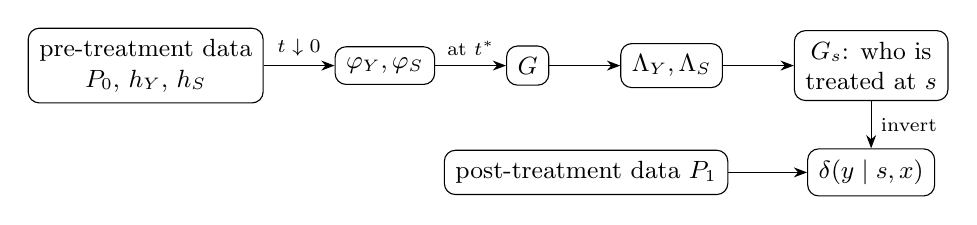
\begin{tikzpicture}[node distance=0.6cm and 0.9cm, box/.style={draw,rounded corners,align=center,font=\small,inner sep=4pt}, >=Stealth]
    \node[box] (pre) {pre-treatment data\\$P_0,\,h_Y,\,h_S$};
    \node[box,right=of pre] (phi) {$\varphi_Y,\varphi_S$};
    \node[box,right=of phi] (G) {$G$};
    \node[box,right=of G] (Lam) {$\Lambda_Y,\Lambda_S$};
    \node[box,right=of Lam] (Gs) {$G_s$: who is\\treated at $s$};
    \node[box,below=of Gs] (delta) {$\delta(y\mid s,x)$};
    \node[box,left=1.0cm of delta] (post) {post-treatment data $P_1$};
    \draw[->] (pre) -- node[above,font=\scriptsize]{$t\downarrow0$} (phi);
    \draw[->] (phi) -- node[above,font=\scriptsize]{at $t^*$} (G);
    \draw[->] (G) -- (Lam);
    \draw[->] (Lam) -- (Gs);
    \draw[->] (Gs) -- node[right,font=\scriptsize]{invert} (delta);
    \draw[->] (post) -- (delta);
  \end{tikzpicture}}

  \raggedright
  \medskip
  \small
  \begin{tabular}{p{0.27\textwidth}p{0.6\textwidth}}
    \toprule
    Assumption & Role \\
    \midrule
    No anticipation & pre-treatment period is a clean competing-risks problem ($\delta$ absent) \\
    Selection only via $(x,V)$ & clocks independent given $V$; treated $=$ risk set reweighted by $V_S$ \\
    MPH separability, $V\perp x$ & index structure $\Lap(\varphi\Lambda)$ behind all three steps \\
    $\E V<\infty$ & step 1 (short-duration hazard ratios) \\
    2-D covariate variation & step 2: trace $\Lap$ on an open set $\Rightarrow$ identifies the dependence \\
    \bottomrule
  \end{tabular}
\note{
\textbf{Use this slide to recap.} If the audience retains one picture, it should be this chain.

Information flows from the pre-treatment data, where nothing causal happens, to the structure of selection. The post-treatment data are then used only once, at the end, to read off $\delta$ after the selection has been removed.

\textbf{What is \emph{not} on the list:} an excluded instrument, selection on observables, parametric functional forms, or multiple spells.
}
\end{frame}

% =====================================================================
\begin{frame}{Heterogeneous effects (Model 1b, Prop.~4)}
  \[
  \theta_Y(t\mid s,x,V)=\begin{cases}\lambda_Y(t)\varphi_Y(x)V_Y & t\le s\\ \lambda_\Delta(t)\varphi_\Delta(x)V_\Delta & t>s\end{cases},
  \qquad (V_Y,V_\Delta,V_S)\sim G_\Delta,
  \]
  \[
  \text{so the effect is}\quad
  \delta(t\mid x,V)=\frac{\lambda_\Delta(t)\varphi_\Delta(x)V_\Delta}{\lambda_Y(t)\varphi_Y(x)V_Y}.
  \]
  \begin{itemize}
    \item \textbf{Gained:} the effect varies with unobservables, and $V_\Delta$ may correlate with $V_S$. This allows \textbf{selection on gains} (Roy-type sorting).
    \item \textbf{Lost:} $\delta$ can no longer depend on the treatment date $s$.
    \item \textbf{Why it works:} after $S$, the residual duration of the treated cohort is again MPH, in $\Lambda_\Delta(y)-\Lambda_\Delta(s)$ with frailty $V_\Delta$, so Elbers--Ridder can be rerun on it.
    \item \textbf{Extra assumptions:} variation in $\varphi_\Delta(x)$, and $\E[V_\Delta V_S]<\infty$. The moment is of the \emph{product} because the treated cohort is tilted by $V_S$.
  \end{itemize}
\note{
\textbf{Why the trade-off arises.} In Model 1a, $\delta(t\mid s,x)$ can be any function, but it is common to all types. Identification inverts $P_1$ for a single unknown function $D$ given a known $G_s$. In Model 1b the post-treatment hazard has its own frailty, so after treatment there is a new unknown distribution (that of $V_\Delta$ in the treated cohort). Identifying it requires running the MPH argument again on post-treatment durations. That argument needs the post-treatment hazard to be proportional and the same function for all $s$, so dependence on $s$ is ruled out.

\textbf{Proof idea (appendix).} Take second derivatives of the data with respect to $(y,s)$. Letting $y,s\downarrow0$ identifies $\varphi_\Delta$ (the analogue of step 1). Then the trivariate Laplace transform is traced on an open set (the analogue of step 2).
}
\end{frame}

% =====================================================================
\begin{frame}{Multiple spells: the within estimator (Model 2c, Prop.~6)}
  Strata (same person twice, siblings, \ldots) with two spells sharing the same unobservables:
  \[ \theta_{Y_k}(t\mid S_k,V)=\lambda_{Y_k}(t)\,V_Y(t)\,\delta_k(t\mid S_k)^{\1\{t>S_k\}},\qquad k=1,2,\quad \lambda_{Y_1}\equiv1. \]
  $V_Y(t)$ may be \textbf{any process common to both spells}, and there is \textbf{no model for $S_k$}.

  \medskip
  Given that the first exit in the stratum happens at $t$, which spell was it? $V_Y(t)$ \textbf{cancels}:
  \[ \Pr(\text{spell 1}\mid t,\text{histories},V)=\frac{\theta_{Y_1}(t)}{\theta_{Y_1}(t)+\theta_{Y_2}(t)}. \]
  \small
  \begin{tabular}{lll}
    \toprule
    treated at $t$ & $\Pr(\text{spell 1 first})$ & identifies \\
    \midrule
    neither & $1/(1+\lambda_{Y_2})$ & $\lambda_{Y_2}$ \\
    spell 1 only & $\delta_1/(\delta_1+\lambda_{Y_2})$ & $\delta_1$ \\
    spell 2 only & $1/(1+\lambda_{Y_2}\delta_2)$ & $\delta_2$ \\
    both & $\delta_1/(\delta_1+\lambda_{Y_2}\delta_2)$ & (overidentifying) \\
    \bottomrule
  \end{tabular}

  \normalsize
  \medskip
  \textbf{Cox partial likelihood $=$ conditional logit $=$ fixed effects.} \textbf{Cost:} $V$ identical across spells, and \textbf{no causal links across spells}.
\note{
\textbf{Why this is the panel analogue.} In linear panels the within transformation removes the individual effect. Here, conditioning on ``one of the two spells ends at $t$'' removes the stratum effect, because it multiplies both hazards. This is Cox's partial-likelihood logic, applied to strata (Holt \& Prentice 1974; Ridder \& Tunal\i{} 1999).

\textbf{What is gained relative to the single-spell case.} No covariates are needed, no finite means, no MPH assumption on how $V$ interacts with time ($V_Y(t)$ can be an arbitrary process), and no model for treatment assignment at all.

\textbf{What it costs.} The unobservable must be \emph{exactly} shared across the two spells. The first spell (or its treatment) must not causally affect the second. For repeated unemployment spells of the same person, that rules out scarring and learning across spells (see the traps discussion on slide 19).

\textbf{Models 2a/2b} (Prop.~5) are MPH versions that also identify $G$; see the appendix.
}
\end{frame}

% =====================================================================
\begin{frame}{What is traded, and critiques}
  \begin{columns}[T]
    \begin{column}{0.45\textwidth}
      \textbf{Not needed}
      \begin{itemize}
        \item an excluded instrument
        \item selection on observables
        \item parametric functional forms
        \item multiple spells (single-spell results)
      \end{itemize}
      \textbf{Needed}
      \begin{itemize}
        \item no anticipation (untestable)
        \item time-invariant unobservables, $V\perp x$
        \item MPH proportionality
        \item 2-D, non-proportional covariate variation
        \item finite means; continuous time
      \end{itemize}
    \end{column}
    \begin{column}{0.53\textwidth}
      \textbf{Critiques}
      \begin{itemize}
        \item Identification comes from $t\downarrow0$, where data are thin. In practice: parametric $\lambda$, discrete $G$ (Heckman--Singer); Monte Carlo evidence in Gaure, R\o ed \& Zhang (2007).
        \item Discrete time: sanction and exit in the same month blur the local signal.
        \item $\delta$ is a hazard ratio \emph{conditional on $V$}. Effects on mean duration or population survival require $G$.
        \item Transitory shocks hitting both hazards (the caseworker reacts to this week's low effort) violate Assn.~2.
      \end{itemize}
    \end{column}
  \end{columns}
\note{
\textbf{One-sentence summary of the trade.} The excluded \emph{variable} is replaced by (i) an excluded timing \emph{shock}, (ii) multiplicative separability, (iii) time-invariant heterogeneity, and (iv) no anticipation.

\textbf{On the last critique.} This is the most common objection in the sanctions literature. Sanctions are typically triggered by observed non-compliance, which may reflect a temporary drop in search effort that also lowers the exit rate. That is a time-varying unobservable affecting both hazards, which Model 1a excludes. Model 2c partly addresses it, but only with multiple spells.
}
\end{frame}

% =====================================================================
\begin{frame}{Connection: staggered adoption DiD}
  \textbf{Same skeleton}
  \begin{itemize}
    \item $Y^*(s)$ $\leftrightarrow$ $Y_t(g)$, potential outcomes indexed by adoption cohort.
    \item No anticipation is \emph{the same assumption} (Callaway \& Sant'Anna 2021; Sun \& Abraham 2021; Borusyak, Jaravel \& Spiess 2024).
    \item The risk set $R_s$ $\leftrightarrow$ the \emph{not-yet-treated} comparison group.
    \item $\delta(t\mid s)$ varies by cohort $s$ and event time $t-s$: the heterogeneity that breaks TWFE.
  \end{itemize}
  \textbf{Differences}
  \begin{itemize}
    \item Selection: \emph{parallel trends} (additive, in levels) vs.\ \emph{time-invariant frailty} (multiplicative, in hazards) plus a random timing shock.
    \item \textbf{Attrition from an absorbing exit:} the treatment changes who remains (slide 13), so ``parallel trends in hazards'' fails \emph{even under random timing}.\\
      DiD on survival probabilities $\to$ a population estimand; ToE $\to$ the individual hazard effect $\delta$, which needs $G$.
    \item If timing is random given observables (\emph{dynamic CIA}), treat later treatment as independent censoring. Population effects on survival are then identified nonparametrically (Fredriksson \& Johansson 2008; Crépon et al.\ 2009; Vikström 2017). ToE is the tool when timing is selected on \emph{unobservables}.
  \end{itemize}
\note{
\textbf{Why the analogy is exact on the skeleton.} Both literatures face a treatment that switches on at a unit-specific date and stays on. Both index potential outcomes by that date. Both impose no anticipation. The comparison ``treated at $s$ vs.\ not yet treated at $s$'' on slide 7 is the event-time-zero comparison of Callaway--Sant'Anna using not-yet-treated controls.

\textbf{Where they part.} In DiD every unit stays in the panel and the outcome is a level. In duration data the outcome is the exit itself, so the sample at risk changes as a \emph{result} of the outcome, and of the treatment. Even if treatment timing were randomly assigned, post-treatment hazard comparisons are contaminated by differential attrition. That is a dynamic-selection bias with no analogue in a balanced panel.

\textbf{Two estimands.} The population effect on survival curves can be obtained by design-based arguments under dynamic CIA. The individual-level hazard effect $\delta$ (needed for structural or behavioural interpretation, e.g.\ search theory) needs a model of $V$.

\textbf{Check citations before the talk.}
}
\end{frame}

% =====================================================================
\begin{frame}{Connection: sequential exogeneity, feedback, and traps}
  \textbf{Sequential exogeneity and feedback}
  \begin{itemize}
    \item A hazard is an intensity relative to the past: $dN_Y(t)-\theta_Y(t\mid\text{past},V)\,dt$ is a martingale difference. This is a continuous-time \emph{sequential moment condition}. No anticipation means treatment is \emph{predetermined}.
    \item In a single absorbing spell, outcome$\to$treatment feedback is degenerate (the only outcome history is ``still here''). The bite is on transitory shocks: $S$ may depend on permanent $V$, not on shocks to the exit rate. This is \emph{strict exogeneity given a fixed effect}.
    \item Model 2c moves toward sequential exogeneity: $S$ is unmodelled and may track a time-varying common $V_Y(t)$, at the cost of needing multiple spells.
  \end{itemize}
  \textbf{Traps: state dependence vs.\ permanent heterogeneity}
  \begin{itemize}
    \item The model separates three objects: $\lambda_Y\downarrow$ (true duration dependence: a trap), $G$ (permanent heterogeneity), and $\delta$ (the effect of an intervention).
    \item Traps suggest \emph{when} you intervene matters: $\delta(t\mid s)$ varying in $s$. Model 1a allows it; Model 1b rules it out.
    \item Multiple-spell results assume no cross-spell effects, i.e.\ they \emph{rule out} lagged duration dependence, the across-spell trap mechanism.
  \end{itemize}
\note{
\textbf{Sequential exogeneity.} In panel data, sequential exogeneity, $\E[u_t\mid x_t,x_{t-1},\ldots,\alpha]=0$, allows future regressors to respond to past outcome shocks (feedback). In counting-process language, the intensity is defined relative to a filtration, and the martingale property is the same type of sequential condition. Treatment history up to $t^-$ can be in the conditioning set, which is exactly no anticipation.

What ToE adds is the fixed effect $V$, together with the assumption that treatment does not respond to transitory shocks that also move the exit hazard. With one spell there is no outcome path to feed back from, except survival itself, so the relevant distinction is permanent vs.\ transitory unobservables. For genuine feedback you need richer outcome histories: multi-state or recurrent events. That leads to the dynamic discrete-choice/treatment literature (Heckman \& Navarro 2007; Abbring \& Heckman 2007, \textit{Handbook of Econometrics} 6B).

\textbf{Traps.} The primer's ``trap or sorting?'' question is the same identification problem as $\lambda$ vs.\ $G$ in the MPH model. Here, as in Heckman's work, it is resolved by proportionality plus short-duration behaviour, or by multiple spells (Honoré 1993). A poverty-trap application would ask whether an intervention's effect depends on how long someone has been poor, which is $s$-dependence of $\delta$. Note the tension: the multiple-spell route, which relaxes the strong single-spell assumptions, assumes away cross-spell scarring, which is one of the main trap channels.

\textbf{Possible extensions to discuss} (my suggestions, not in the paper): ToE with lagged occurrence dependence across spells; ToE estimands vs.\ DiD estimands on the same data; anticipation as an information shock with observed notification dates.
}
\end{frame}

% =====================================================================
\begin{frame}{Takeaways}
  \begin{enumerate}
    \item \textbf{Timing is information.} Treatment acts only after $S$, while unobservables act throughout. Causal effects are \emph{local}; selection is \emph{global}.
    \item \textbf{The pre-treatment period is a competing-risks experiment with no treatment effect in it.} With MPH structure and non-proportional covariate variation, it reveals who is at risk and who gets treated ($G$). Knowing $G$ strips out selection into treatment and selection out of the risk set afterwards.
    \item \textbf{The price.} No anticipation, multiplicative separability, time-invariant heterogeneity, and a timing shock that is excluded from the outcome. Multiple spells buy back generality at the cost of no cross-spell dynamics.
  \end{enumerate}
\note{
Leave time for discussion. Good questions to put to the group:
(1) In your application, is the timing shock plausibly excluded?
(2) Is $\delta$ (a hazard ratio given $V$) the parameter you care about, or a population survival effect?
(3) What would anticipation look like, and do you observe notification dates?
}
\end{frame}

% =====================================================================
\appendix
\begin{frame}{Appendix A: non-identification (Prop.~1) and the job-search example}
  \centering
  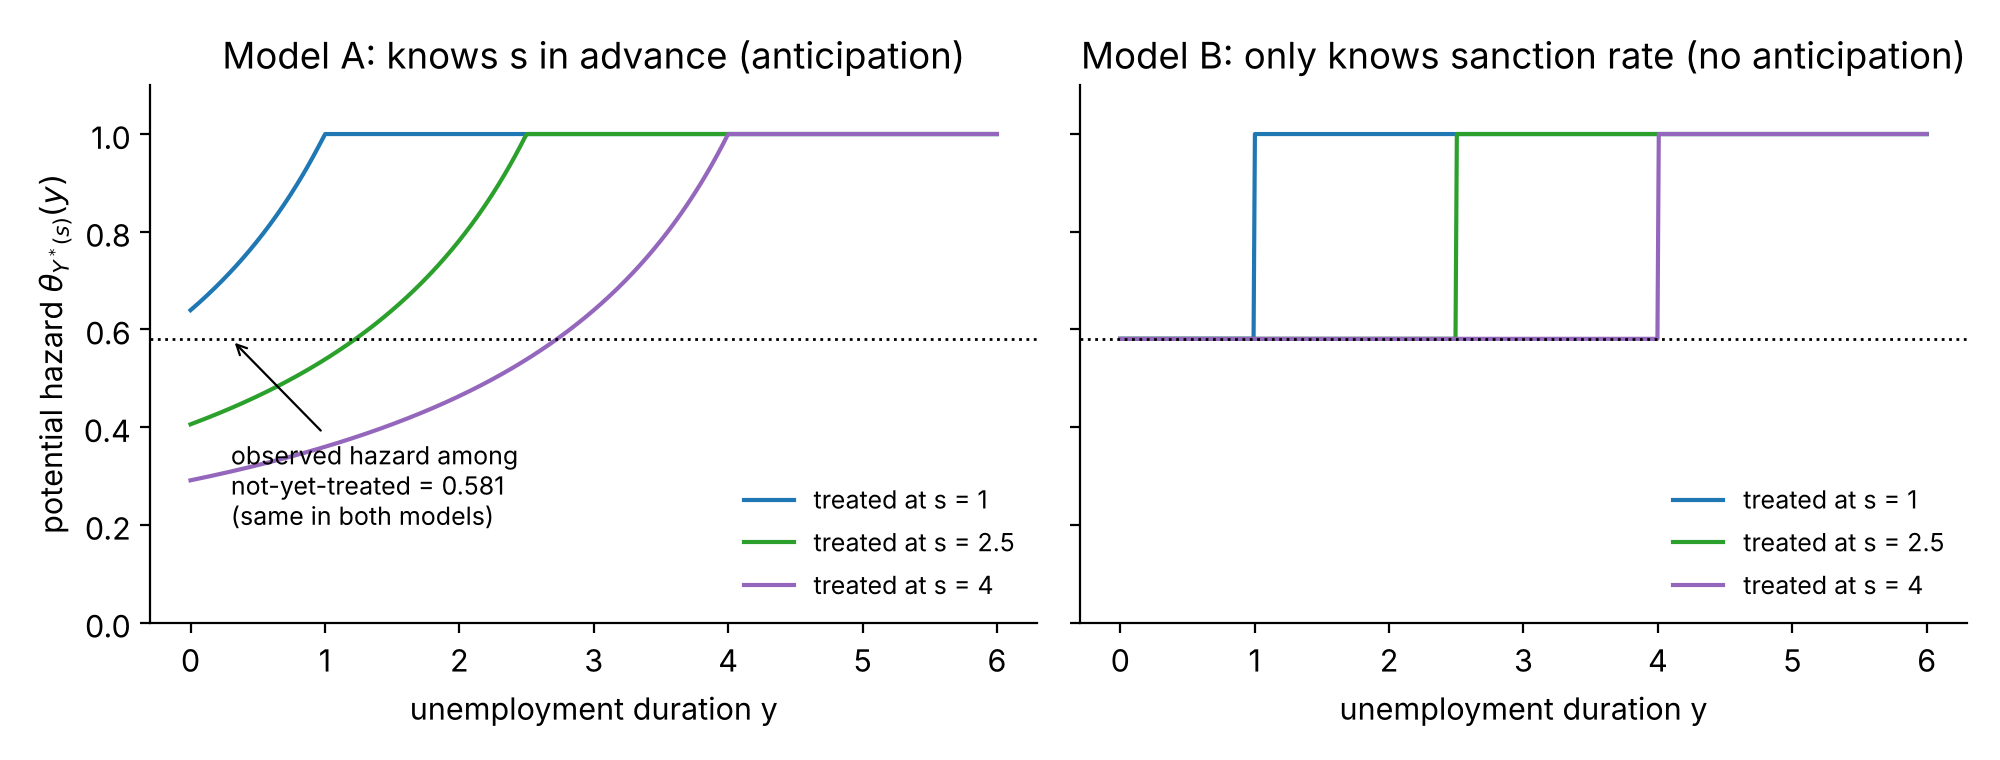
\includegraphics[width=0.82\linewidth]{fig2_anticipation_equivalence.png}

  \raggedright\small
  Model A: the worker knows the sanction date $s$, and search effort (hence the hazard) rises before $s$. Model B: only the sanction rate is known, so the hazard jumps at $s$. With suitably chosen parameters the two produce \emph{identical} data. The data only reveal the hazard among the not-yet-treated (0.581 in both).

  \smallskip
  \textbf{Proof of Prop.~1.} By Tsiatis/Miller there is an independent pair $(\hat Y,\hat S)$ matching the competing-risks part. Use $\hat S$ as the treatment and $\hat Y$'s hazard before treatment for every $Y^*(s)$; define post-treatment hazards from $P_1$.
\note{
Parameters: $w=1$, $b=1/2$. Model A has a discount rate of 5\%; Model B has a discount rate of 1.23\% and a sanction rate of 0.419. Equation (3) of the paper gives Model A's hazard; footnote 11 derives the common observed hazard.
}
\end{frame}

\begin{frame}{Appendix B: data objects vs.\ the paper's $(Q_S,Q_Y)$}
  The paper's data: $Q_S(y,s)=\Pr(Y>y,S>s,Y>S)$ and $Q_Y(y)=\Pr(Y>y,Y<S)$. Then
  \begin{align*}
    P_0(t)&=Q_S(t,t)+Q_Y(t),\\
    h_Y(t)&=-Q_Y'(t)/P_0(t),\qquad h_S(t)=-\partial_sQ_S(t,s)\big|_{s=t}\big/P_0(t),\\
    P_1(y\mid s)&=\partial_sQ_S(y,s)\big/\partial_sQ_S(s,s)\qquad(y>s).
  \end{align*}
  Conversely, $(P_0,h_Y,h_S,P_1)$ determine $(Q_S,Q_Y)$. The objects are equivalent.
\end{frame}

\begin{frame}{Appendix C: uniqueness in step 3}
  Suppose $(a,b)\neq(a',b')$ both satisfy $P_0(t\mid x)=\Lap(\varphi_Y(x)a,\varphi_S(x)b)$ for all $x$. Then $\Lap(pa,qb)=\Lap(pa',qb')$ on an open set of $(p,q)$. By analyticity,
  \[ \Lap(u,v)=\Lap(ku,mv)\quad\text{for all }(u,v)\in(0,\infty)^2,\qquad k=a'/a,\ m=b'/b,\ (k,m)\neq(1,1). \]
  \begin{itemize}
    \item $k,m\ge1$ (or both $\le1$): contradicts $\Lap$ strictly decreasing in each argument (needs $\Pr(V\in(0,\infty)^2)>0$).
    \item $k>1>m$: iterating gives $\Lap(u,v)=\Lap(k^nu,m^nv)\to\Pr(V_Y=0)$ as $n\to\infty$. So $\Lap$ is constant, a contradiction. The case $k<1<m$ is symmetric.
  \end{itemize}
\end{frame}

\begin{frame}{Appendix D: proof sketches for Models 1b, 2a, 2b}
  \small
  \textbf{Model 1b (Prop.~4).} After Prop.~2, for $y>s$:
  \[ \frac{\partial^2Q_S(y,s\mid x)/\partial y\partial s}{\partial^2Q_S(y,s\mid x^*)/\partial y\partial s}\;\xrightarrow{\;y,s\downarrow0\;}\;\varphi_S(x)\varphi_\Delta(x) \quad(\text{needs }\E[V_\Delta V_S]<\infty), \]
  which identifies $\varphi_\Delta$. Then $\partial_sQ_S/(\lambda_S\varphi_S)=\Lap^{(S)}_{G_\Delta}\big(\varphi_Y\Lambda_Y(s),\varphi_\Delta(\Lambda_\Delta(y)-\Lambda_\Delta(s)),\varphi_S\Lambda_S(s)\big)$. Let $s\downarrow0$ to get $\Lambda_\Delta$; vary $x,y$ to trace $\Lap_{G_\Delta}$ on an open set.

  \medskip
  \textbf{Models 2a/2b (Prop.~5).} Two spells per stratum sharing $V=(V_Y,V_S)$ (or $(V_Y,V_\Delta,V_S)$), spell-specific baselines and effects. The two-spell competing-risks structure identifies $\Lambda_{Y_k},\Lambda_{S_k}$ (Abbring \& Van den Berg 2003, JRSSB). The extra cross-spell information then identifies $\delta_k$ and $G$, \textbf{without covariates and without finite means}, mirroring Honoré (1993).
\end{frame}

\end{document}
